% $Author: luc $
% $Date: 2010-08-01 13:46:12 +0100 $
% $Revision: 0 $

% HISTORY:
% 2010-08-01 - Luc
%% 2011-09-11 - Migrated to PharoBox: svn checkout https://XXX@scm.gforge.inria.fr/svn/pharobooks/PharoByExampleTwo-Eng

%=================================================================
\ifx\wholebook\relax\else
% --------------------------------------------
% Lulu:
	\documentclass[a4paper,10pt,twoside]{book}
	\usepackage[
		papersize={6.13in,9.21in},
		hmargin={.75in,.75in},
		vmargin={.75in,1in},
		ignoreheadfoot
	]{geometry}
	% $Author$
% $Date$
% $Revision$

% HISTORY:
% 2006-10-31 - Oscar code macros
% ...

%=============================================================
% NB: documentclass must be set in main document.
% Allows book to be generated in multiple formats.
%=============================================================
%:Packages
\usepackage[T1]{fontenc}  %%%%%% really important to get the code directly in the text!
\usepackage{lmodern}
%\usepackage[scaled=0.85]{bookmanx} % needs another scale factor if used with \renewcommand{\sfdefault}{cmbr}
\usepackage{palatino}
\usepackage[scaled=0.85]{helvet}
\usepackage[protrusion,expansion=false]{microtype}
\usepackage{graphicx}
\usepackage{theorem}
\usepackage[english]{babel}
% ON: pdfsync breaks the use of p{width} for tabular columns!
\ifdefined\usepdfsync\usepackage{pdfsync}\fi % Requires texlive 2007
%=============================================================
%:More packages
%Stef should check which ones are used!
%\usepackage{picinpar}
%\usepackage{layout}
%\usepackage{color}
%\usepackage{enum}
%\usepackage{a4wide}
% \usepackage{fancyhdr}
\usepackage{ifthen}
\usepackage{float}
\usepackage{longtable}
\usepackage{makeidx}
\usepackage[nottoc]{tocbibind}
\usepackage{multicol}
\usepackage{booktabs}	% book-style tables
\usepackage{topcapt}	% enables \topcaption
\usepackage{multirow}
\usepackage{tabularx}
%\usepackage[bottom]{footmisc}
\usepackage{xspace}
\usepackage{alltt}
\usepackage{amssymb,textcomp}
\usepackage[usenames,dvipsnames]{color}
%\usepackage{colortbl}
\usepackage[hang]{subfigure}\makeatletter\def\p@subfigure{\thefigure\,}\makeatother
\usepackage{rotating}
\usepackage{enumitem}	% apb: allows more control over tags in enumerations
\usepackage{verbatim}     % for comment environment
\usepackage{varioref}	% for page references that work
\labelformat{footnote}{\thechapter--#1} % to distinguish citations from jurabib
\usepackage{needspace}
\usepackage{isodateo} % enable \isodate
\usepackage[newparttoc,pagestyles]{titlesec}
\usepackage{titletoc}
\usepackage{wrapfig}

\usepackage[
	super,
	citefull=first,
	authorformat={allreversed,and},
	titleformat={commasep,italic}
]{jurabib} % citations as footnotes
\usepackage[
	colorlinks=true,
	linkcolor=black,
	urlcolor=black,
	citecolor=black
]{hyperref}   % should come last
%=============================================================
%:PDF version
\pdfminorversion=3 % Set PDF to 1.3 for Lulu
%=============================================================
%:URL style
\makeatletter
\def\url@leostyle{%
  \@ifundefined{selectfont}{\def\UrlFont{\sf}}{\def\UrlFont{\sffamily}}}
\makeatother
% Now actually use the newly defined style.
\urlstyle{leo}
%=============================================================
%:Booleans
\newboolean{lulu}
\setboolean{lulu}{false}
\newcommand{\ifluluelse}[2]{\ifthenelse{\boolean{lulu}}{#1}{#2}}
%=============================================================
%:Names
\newcommand{\SUnit}{SUnit\xspace}
\newcommand{\sunit}{SUnit\xspace}
\newcommand{\xUnit}{$x$Unit\xspace}
\newcommand{\JUnit}{JUnit\xspace}
\newcommand{\st}{Smalltalk\xspace}
\newcommand{\pharo}{Pharo\xspace} % Use this, not \Pharo
%\newcommand{\sqmap}{SqueakMap\xspace}
\newcommand{\squeak}{Squeak\xspace} % use this, not \Squeak or \sq
\newcommand{\sqsrc}{SqueakSource\xspace}
\newcommand{\sbe}{\url{http://SqueakByExample.org}\xspace}
\newcommand{\pharoweb}{\url{http://pharo-project.org}\xspace}
\newcommand{\pbe}{\url{http://PharoByExample.org}\xspace}
\newcommand{\sba}{\url{http://SquareBracketAssociates.org}\xspace}
\newcommand{\bam}{\lct{Bounc\-ing\-Atoms\-Morph}\xspace}
%=============================================================
%:Markup macros for proof-reading
\usepackage[normalem]{ulem} % for \sout
\usepackage{xcolor}
\newcommand{\ra}{$\rightarrow$}
\newcommand{\ugh}[1]{\textcolor{red}{\uwave{#1}}} % please rephrase
\newcommand{\ins}[1]{\textcolor{blue}{\uline{#1}}} % please insert
\newcommand{\del}[1]{\textcolor{red}{\sout{#1}}} % please delete
\newcommand{\chg}[2]{\textcolor{red}{\sout{#1}}{\ra}\textcolor{blue}{\uline{#2}}} % please change
%=============================================================
%:Editorial comment macros
%\newcommand{\nnbb}[2]{
%    % \fbox{\bfseries\sffamily\scriptsize#1}
%    \fcolorbox{gray}{yellow}{\bfseries\sffamily\scriptsize#1}
%    {\sf\small$\blacktriangleright$\textit{#2}$\blacktriangleleft$}
%   }
\newcommand{\yellowbox}[1]{\fcolorbox{gray}{yellow}{\bfseries\sffamily\scriptsize#1}}
\newcommand{\triangles}[1]{{\sf\small$\blacktriangleright$\textit{#1}$\blacktriangleleft$}}
\newcommand{\nnbb}[2]{\yellowbox{#1} \triangles{#2}}
\newcommand{\fix}{\yellowbox{FIX!}}
\newcommand{\here}{\yellowbox{CONTINUE HERE!}}
% editor macros
\newcommand{\apl}[1]{\nnbb{Alain}{#1}} % Alain
\newcommand{\ab}[1]{\nnbb{Andrew}{#1}} % Black
\newcommand{\sd}[1]{\nnbb{St\'{e}f}{#1}} % Ducasse
\newcommand{\gl}[1]{\nnbb{Guillaume}{#1}} % Ducasse
\newcommand{\cd}[1]{\nnbb{Christophe}{#1}} % Ducasse
\newcommand{\sig}[1]{\nnbb{Igor}{#1}} % Igor
\newcommand{\dc}[1]{\nnbb{DamienC}{#1}} % Ducasse
\newcommand{\md}[1]{\nnbb{Marcus}{#1}} % Denker
\newcommand{\on}[1]{\nnbb{Oscar}{#1}} % Nierstrasz
\newcommand{\damien}[1]{\nnbb{Damien}{#1}} % Pollet
\newcommand{\lr}[1]{\nnbb{Lukas}{#1}} % Renggli
\newcommand{\orla}[1]{\nnbb{Orla}{#1}} % Greevy
\newcommand{\alex}[1]{\nnbb{Alex}{#1}} % Bergel
\newcommand{\alx}[1]{\nnbb{Alex}{#1}} % Bergel
\newcommand{\dr}[1]{\nnbb{David}{#1}} % Roethlisberger
\newcommand{\ja}[1]{\nnbb{Jannik}{#1}} % Laval
\newcommand{\cb}[1]{\nnbb{Camillo}{#1}} % Bruni
\newcommand{\jr}[1]{\nnbb{Jorge}{#1}} % Ressia
\newcommand{\jb}[1]{\nnbb{JB}{#1}} % JB
\newcommand{\jp}[1]{\nnbb{Javier}{#1}} % Pimas
\newcommand{\fp}[1]{\nnbb{Fabrizio}{#1}} % Perin
\newcommand{\michael}[1]{\nnbb{Michael}{#1}} % Davies
\newcommand{\ew}[1]{\nnbb{Erwann}{#1}} % Wernli
\newcommand{\mb}[1]{\nnbb{Martial}{#1}} % Boniou
\newcommand{\hw}[1]{\nnbb{Hernan}{#1}} % Wilkinson
\newcommand{\ben}[1]{\nnbb{Benjamin}{#1}} % Benjamin Van Ryseghem
\newcommand{\hjo}[1]{\nnbb{HwaJong}{#1}} % HwaJong Oh aka daliot
\newcommand{\ml}[1]{\nnbb{Max}{#1}} % Max Leske
\newcommand{\mmp}[1]{\nnbb{Mariano}{#1}} % Mariano Martinez Peck
\newcommand{\luc}[1]{\nnbb{Luc}{#1}} % Luc Fabresse
\newcommand{\dkl}[1]{\nnbb{Daniel}{#1}} % Daniel Lyons
\newcommand{\vu}[1]{\nnbb{Veronica}{#1}} % Veronica Uquillas Gomez
\newcommand{\martin}[1]{\nnbb{Martin}{#1}} % Martin Dias
\newcommand{\vp}[1]{\nnbb{Vanessa}{#1}} % Vanessa Pena
\newcommand{\gp}[1]{\nnbb{Guille}{#1}} % Guillermo Polito

%=============================================================
%:Abbreviation macros
\newcommand{\ie}{\emph{i.e.},\xspace}
\newcommand{\eg}{\emph{e.g.},\xspace}
\newcommand{\etc}{etc.\xspace}
%=============================================================
%:Cross reference macros
\newcommand{\charef}[1]{Chapter~\ref{cha:#1}\xspace}
\newcommand{\secref}[1]{Section~\ref{sec:#1}\xspace}
\newcommand{\figref}[1]{Figure~\ref{fig:#1}\xspace}
\newcommand{\Figref}[1]{Figure~\ref{fig:#1}\xspace}
\newcommand{\appref}[1]{Appendix~\ref{app:#1}\xspace}
\newcommand{\tabref}[1]{Table~\ref{tab:#1}\xspace}
\newcommand{\faqref}[1]{FAQ~\ref{faq:#1}, p.~\pageref{faq:#1}\xspace}
% APB: I removed trailing \xspace commands from these macros because
% \xspace mostly doesn't work.  If you want a space after your
% references, type one!
% ON: xspace has always worked just fine for me!  Please leave them in.
%
\newcommand{\ruleref}[1]{\ref{rule:#1}\xspace}
%
\newcommand{\egref}[1]{example~\ref{eg:#1}\xspace}
\newcommand{\Egref}[1]{Example~\ref{eg:#1}\xspace}
%
\newcommand{\scrref}[1]{script~\ref{scr:#1}\xspace}
\newcommand{\Scrref}[1]{Script~\ref{scr:#1}\xspace}
\newcommand{\tscrref}[1]{the script~\ref{scr:#1}\xspace}
\newcommand{\Tscrref}[1]{The script~\ref{scr:#1}\xspace}
%
\newcommand{\mthref}[1]{method~\ref{mth:#1}\xspace}
\newcommand{\mthsref}[1]{methods~\ref{mth:#1}\xspace}
\newcommand{\Mthref}[1]{Method~\ref{mth:#1}\xspace}
\newcommand{\tmthref}[1]{the method~\ref{mth:#1}\xspace}
\newcommand{\Tmthref}[1]{The method~\ref{mth:#1}\xspace}
%
\newcommand{\clsref}[1]{class~\ref{cls:#1}\xspace}
\newcommand{\tclsref}[1]{the class~\ref{cls:#1}\xspace}
\newcommand{\Tclsref}[1]{The class~\ref{cls:#1}\xspace}

\newcommand{\chalabel}[1]{\label{cha:#1}}
\newcommand{\seclabel}[1]{\label{sec:#1}}
\newcommand{\figlabel}[1]{\label{fig:#1}}
\newcommand{\tablabel}[1]{\label{tab:#1}}
\newcommand{\rulelabel}[1]{\label{rule:#1}}
\newcommand{\eglabel}[1]{\label{eg:#1}}
\newcommand{\scrlabel}[1]{\label{scr:#1}}
\newcommand{\mthlabel}[1]{\label{mth:#1}}
\newcommand{\clslabel}[1]{\label{cls:#1}}
\newcommand{\faqlabel}[1]{\label{faq:#1}}
%=============================================================
%:Menu item macro
% for menu items, so we can change our minds on how to print them! (apb)
\definecolor{lightgray}{gray}{0.89}
\newcommand{\menu}[1]{{%
	\setlength{\fboxsep}{0pt}%
	\colorbox{lightgray}{{{\upshape\sffamily\strut \,#1\,}}}}}
\newcommand{\link}[1]{{%
	\fontfamily{lmr}\selectfont
 	\upshape{\sffamily \underline{#1}}}}
% For submenu items:
\newcommand{\go}{\,$\triangleright$\,}
% \newcommand{\go}{\,$\blacktriangleright$\,}
% For keyboard shortcuts:
%\newcommand{\short}[1]{\mbox{$\langle${\sc CMD}$\rangle$-#1}\xspace}
\newcommand{\short}[1]{\mbox{{\sc cmd}\hspace{0.08em}--\hspace{0.09em}#1}\xspace}
% For buttons:
\newcommand{\button}[1]{{%
	\setlength{\fboxsep}{0pt}%
	\fbox{{\upshape\sffamily\strut \,#1\,}}}}
% NB: The button macro does not work within captions -- incompatible with xcolor package :-(
\newcommand{\toolsflap}{\textit{Tools} flap\xspace}
%=============================================================
%:Mouse clicks
\newcommand{\click}{click\xspace} % RED
\newcommand{\actclick}{action-click\xspace} % YELLOW
\newcommand{\metaclick}{meta-click\xspace} % BLUE
\newcommand{\Click}{Click\xspace} % RED
\newcommand{\Actclick}{Action-click\xspace} % YELLOW
\newcommand{\Metaclick}{Meta-click\xspace} % BLUE
%=============================================================
%:ToSh macros
\newboolean{tosh}
\setboolean{tosh}{false}
\newcommand{\iftoshelse}[2]{\ifthenelse{\boolean{tosh}}{#1}{#2}}
%=============================================================
%:ToSh colors
%\newcommand{\highlightcolor}{\color{blue!65}}
%\newcommand{\boxcolor}{\color{gray!25}}
\newcommand{\highlight}[1]{\textcolor{blue!65}{#1}}
%\newcommand{\codecolor}{\color{blue!65}}
%%\setlength{\fboxrule}{2pt}
%\newcommand{\asPict}[1]{%
%	{\Large\highlight{#1}}}
%=============================================================
%:Reader cues (do this)
%
% Indicate something the reader should try out.
% \newcommand{\dothisicon}{\raisebox{-.5ex}{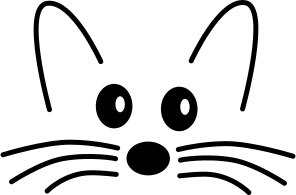
\includegraphics[width=1.4em]{squeak-logo}}}
\iftoshelse{
	\usepackage{marginnote}
		\renewcommand*{\marginfont}{\footnotesize}
	\newcommand{\vartriangleout}{\ifthenelse{\isodd{\thepage}}{\vartriangleright}{\vartriangleleft}}
	\newcommand{\dothisicon}{\fcolorbox{blue!65}{white}{\highlight{$\vartriangleout$}}}
	\newcommand{\dothis}[1]{%
		\noindent\par\noindent
		{\reversemarginpar
			\marginnote{\fcolorbox{blue!65}{white}{\highlight{$\vartriangleout$}}}}
		%\MarginLabel{do this}
		\noindent\emph{#1}
		\nopagebreak}
}{
	\newcommand{\dothisicon}{\raisebox{-.5ex}{
\includegraphics[height=1.2em]{pharo}}}
	\newcommand{\dothis}[1]{%
		\medskip
		\noindent\dothisicon
		\ifx#1\empty\else\quad\emph{#1}\fi
		\par\smallskip\nopagebreak}
}
%===> NEW VERSION <===
% NB: To use this in an individual chapter, you must set:
%\graphicspath{{figures/} {../figures/}}
% at the head of the chapter.  Don't forget the final /
%=============================================================
%:Reader hints (hint)
%
% Indicates a non-obvious consequence
\newcommand{\hint}[1]{\vspace{1ex}\noindent\fbox{\textsc{Hint}} \emph{#1}}
%=================================================================
% graphics for Morphic handles
\newcommand{\grabHandle}{\raisebox{-0.2ex}{
\includegraphics[width=1em]{blackHandle}}}
\newcommand{\moveHandle}{\raisebox{-0.2ex}{
\includegraphics[width=1em]{moveHandle}}}
\newcommand{\debugHandle}{\raisebox{-0.2ex}{
\includegraphics[width=1em]{debugHandle}}}
%=============================================================
%:Highlighting Important stuff (doublebox)
%
% From Seaside book ...
\newsavebox{\SavedText}
\newlength{\InnerBoxRule}\setlength{\InnerBoxRule}{.75\fboxrule}
\newlength{\OuterBoxRule}\setlength{\OuterBoxRule}{1.5\fboxrule}
\newlength{\BoxSeparation}\setlength{\BoxSeparation}{1.5\fboxrule}
\addtolength{\BoxSeparation}{.5pt}
\newlength{\SaveBoxSep}\setlength{\SaveBoxSep}{2\fboxsep}
%
\newenvironment{doublebox}{\begin{lrbox}{\SavedText}
    \begin{minipage}{.75\textwidth}}
    {\end{minipage}\end{lrbox}\begin{center}
    \setlength{\fboxsep}{\BoxSeparation}\setlength{\fboxrule}{\OuterBoxRule}
    \fbox{\setlength{\fboxsep}{\SaveBoxSep}\setlength{\fboxrule}{\InnerBoxRule}%
      \fbox{\usebox{\SavedText}}}
  \end{center}}
% Use this:
\newcommand{\important}[1]{\begin{doublebox}#1\end{doublebox}}
%=============================================================
%:Section depth
\setcounter{secnumdepth}{2}
%% for this to happen start the file with
%\ifx\wholebook\relax\else
%% $Author$
% $Date$
% $Revision$

% HISTORY:
% 2006-10-31 - Oscar code macros
% ...

%=============================================================
% NB: documentclass must be set in main document.
% Allows book to be generated in multiple formats.
%=============================================================
%:Packages
\usepackage[T1]{fontenc}  %%%%%% really important to get the code directly in the text!
\usepackage{lmodern}
%\usepackage[scaled=0.85]{bookmanx} % needs another scale factor if used with \renewcommand{\sfdefault}{cmbr}
\usepackage{palatino}
\usepackage[scaled=0.85]{helvet}
\usepackage[protrusion,expansion=false]{microtype}
\usepackage{graphicx}
\usepackage{theorem}
\usepackage[english]{babel}
% ON: pdfsync breaks the use of p{width} for tabular columns!
\ifdefined\usepdfsync\usepackage{pdfsync}\fi % Requires texlive 2007
%=============================================================
%:More packages
%Stef should check which ones are used!
%\usepackage{picinpar}
%\usepackage{layout}
%\usepackage{color}
%\usepackage{enum}
%\usepackage{a4wide}
% \usepackage{fancyhdr}
\usepackage{ifthen}
\usepackage{float}
\usepackage{longtable}
\usepackage{makeidx}
\usepackage[nottoc]{tocbibind}
\usepackage{multicol}
\usepackage{booktabs}	% book-style tables
\usepackage{topcapt}	% enables \topcaption
\usepackage{multirow}
\usepackage{tabularx}
%\usepackage[bottom]{footmisc}
\usepackage{xspace}
\usepackage{alltt}
\usepackage{amssymb,textcomp}
\usepackage[usenames,dvipsnames]{color}
%\usepackage{colortbl}
\usepackage[hang]{subfigure}\makeatletter\def\p@subfigure{\thefigure\,}\makeatother
\usepackage{rotating}
\usepackage{enumitem}	% apb: allows more control over tags in enumerations
\usepackage{verbatim}     % for comment environment
\usepackage{varioref}	% for page references that work
\labelformat{footnote}{\thechapter--#1} % to distinguish citations from jurabib
\usepackage{needspace}
\usepackage{isodateo} % enable \isodate
\usepackage[newparttoc,pagestyles]{titlesec}
\usepackage{titletoc}
\usepackage{wrapfig}

\usepackage[
	super,
	citefull=first,
	authorformat={allreversed,and},
	titleformat={commasep,italic}
]{jurabib} % citations as footnotes
\usepackage[
	colorlinks=true,
	linkcolor=black,
	urlcolor=black,
	citecolor=black
]{hyperref}   % should come last
%=============================================================
%:PDF version
\pdfminorversion=3 % Set PDF to 1.3 for Lulu
%=============================================================
%:URL style
\makeatletter
\def\url@leostyle{%
  \@ifundefined{selectfont}{\def\UrlFont{\sf}}{\def\UrlFont{\sffamily}}}
\makeatother
% Now actually use the newly defined style.
\urlstyle{leo}
%=============================================================
%:Booleans
\newboolean{lulu}
\setboolean{lulu}{false}
\newcommand{\ifluluelse}[2]{\ifthenelse{\boolean{lulu}}{#1}{#2}}
%=============================================================
%:Names
\newcommand{\SUnit}{SUnit\xspace}
\newcommand{\sunit}{SUnit\xspace}
\newcommand{\xUnit}{$x$Unit\xspace}
\newcommand{\JUnit}{JUnit\xspace}
\newcommand{\st}{Smalltalk\xspace}
\newcommand{\pharo}{Pharo\xspace} % Use this, not \Pharo
%\newcommand{\sqmap}{SqueakMap\xspace}
\newcommand{\squeak}{Squeak\xspace} % use this, not \Squeak or \sq
\newcommand{\sqsrc}{SqueakSource\xspace}
\newcommand{\sbe}{\url{http://SqueakByExample.org}\xspace}
\newcommand{\pharoweb}{\url{http://pharo-project.org}\xspace}
\newcommand{\pbe}{\url{http://PharoByExample.org}\xspace}
\newcommand{\sba}{\url{http://SquareBracketAssociates.org}\xspace}
\newcommand{\bam}{\lct{Bounc\-ing\-Atoms\-Morph}\xspace}
%=============================================================
%:Markup macros for proof-reading
\usepackage[normalem]{ulem} % for \sout
\usepackage{xcolor}
\newcommand{\ra}{$\rightarrow$}
\newcommand{\ugh}[1]{\textcolor{red}{\uwave{#1}}} % please rephrase
\newcommand{\ins}[1]{\textcolor{blue}{\uline{#1}}} % please insert
\newcommand{\del}[1]{\textcolor{red}{\sout{#1}}} % please delete
\newcommand{\chg}[2]{\textcolor{red}{\sout{#1}}{\ra}\textcolor{blue}{\uline{#2}}} % please change
%=============================================================
%:Editorial comment macros
%\newcommand{\nnbb}[2]{
%    % \fbox{\bfseries\sffamily\scriptsize#1}
%    \fcolorbox{gray}{yellow}{\bfseries\sffamily\scriptsize#1}
%    {\sf\small$\blacktriangleright$\textit{#2}$\blacktriangleleft$}
%   }
\newcommand{\yellowbox}[1]{\fcolorbox{gray}{yellow}{\bfseries\sffamily\scriptsize#1}}
\newcommand{\triangles}[1]{{\sf\small$\blacktriangleright$\textit{#1}$\blacktriangleleft$}}
\newcommand{\nnbb}[2]{\yellowbox{#1} \triangles{#2}}
\newcommand{\fix}{\yellowbox{FIX!}}
\newcommand{\here}{\yellowbox{CONTINUE HERE!}}
% editor macros
\newcommand{\apl}[1]{\nnbb{Alain}{#1}} % Alain
\newcommand{\ab}[1]{\nnbb{Andrew}{#1}} % Black
\newcommand{\sd}[1]{\nnbb{St\'{e}f}{#1}} % Ducasse
\newcommand{\gl}[1]{\nnbb{Guillaume}{#1}} % Ducasse
\newcommand{\cd}[1]{\nnbb{Christophe}{#1}} % Ducasse
\newcommand{\sig}[1]{\nnbb{Igor}{#1}} % Igor
\newcommand{\dc}[1]{\nnbb{DamienC}{#1}} % Ducasse
\newcommand{\md}[1]{\nnbb{Marcus}{#1}} % Denker
\newcommand{\on}[1]{\nnbb{Oscar}{#1}} % Nierstrasz
\newcommand{\damien}[1]{\nnbb{Damien}{#1}} % Pollet
\newcommand{\lr}[1]{\nnbb{Lukas}{#1}} % Renggli
\newcommand{\orla}[1]{\nnbb{Orla}{#1}} % Greevy
\newcommand{\alex}[1]{\nnbb{Alex}{#1}} % Bergel
\newcommand{\alx}[1]{\nnbb{Alex}{#1}} % Bergel
\newcommand{\dr}[1]{\nnbb{David}{#1}} % Roethlisberger
\newcommand{\ja}[1]{\nnbb{Jannik}{#1}} % Laval
\newcommand{\cb}[1]{\nnbb{Camillo}{#1}} % Bruni
\newcommand{\jr}[1]{\nnbb{Jorge}{#1}} % Ressia
\newcommand{\jb}[1]{\nnbb{JB}{#1}} % JB
\newcommand{\jp}[1]{\nnbb{Javier}{#1}} % Pimas
\newcommand{\fp}[1]{\nnbb{Fabrizio}{#1}} % Perin
\newcommand{\michael}[1]{\nnbb{Michael}{#1}} % Davies
\newcommand{\ew}[1]{\nnbb{Erwann}{#1}} % Wernli
\newcommand{\mb}[1]{\nnbb{Martial}{#1}} % Boniou
\newcommand{\hw}[1]{\nnbb{Hernan}{#1}} % Wilkinson
\newcommand{\ben}[1]{\nnbb{Benjamin}{#1}} % Benjamin Van Ryseghem
\newcommand{\hjo}[1]{\nnbb{HwaJong}{#1}} % HwaJong Oh aka daliot
\newcommand{\ml}[1]{\nnbb{Max}{#1}} % Max Leske
\newcommand{\mmp}[1]{\nnbb{Mariano}{#1}} % Mariano Martinez Peck
\newcommand{\luc}[1]{\nnbb{Luc}{#1}} % Luc Fabresse
\newcommand{\dkl}[1]{\nnbb{Daniel}{#1}} % Daniel Lyons
\newcommand{\vu}[1]{\nnbb{Veronica}{#1}} % Veronica Uquillas Gomez
\newcommand{\martin}[1]{\nnbb{Martin}{#1}} % Martin Dias
\newcommand{\vp}[1]{\nnbb{Vanessa}{#1}} % Vanessa Pena
\newcommand{\gp}[1]{\nnbb{Guille}{#1}} % Guillermo Polito

%=============================================================
%:Abbreviation macros
\newcommand{\ie}{\emph{i.e.},\xspace}
\newcommand{\eg}{\emph{e.g.},\xspace}
\newcommand{\etc}{etc.\xspace}
%=============================================================
%:Cross reference macros
\newcommand{\charef}[1]{Chapter~\ref{cha:#1}\xspace}
\newcommand{\secref}[1]{Section~\ref{sec:#1}\xspace}
\newcommand{\figref}[1]{Figure~\ref{fig:#1}\xspace}
\newcommand{\Figref}[1]{Figure~\ref{fig:#1}\xspace}
\newcommand{\appref}[1]{Appendix~\ref{app:#1}\xspace}
\newcommand{\tabref}[1]{Table~\ref{tab:#1}\xspace}
\newcommand{\faqref}[1]{FAQ~\ref{faq:#1}, p.~\pageref{faq:#1}\xspace}
% APB: I removed trailing \xspace commands from these macros because
% \xspace mostly doesn't work.  If you want a space after your
% references, type one!
% ON: xspace has always worked just fine for me!  Please leave them in.
%
\newcommand{\ruleref}[1]{\ref{rule:#1}\xspace}
%
\newcommand{\egref}[1]{example~\ref{eg:#1}\xspace}
\newcommand{\Egref}[1]{Example~\ref{eg:#1}\xspace}
%
\newcommand{\scrref}[1]{script~\ref{scr:#1}\xspace}
\newcommand{\Scrref}[1]{Script~\ref{scr:#1}\xspace}
\newcommand{\tscrref}[1]{the script~\ref{scr:#1}\xspace}
\newcommand{\Tscrref}[1]{The script~\ref{scr:#1}\xspace}
%
\newcommand{\mthref}[1]{method~\ref{mth:#1}\xspace}
\newcommand{\mthsref}[1]{methods~\ref{mth:#1}\xspace}
\newcommand{\Mthref}[1]{Method~\ref{mth:#1}\xspace}
\newcommand{\tmthref}[1]{the method~\ref{mth:#1}\xspace}
\newcommand{\Tmthref}[1]{The method~\ref{mth:#1}\xspace}
%
\newcommand{\clsref}[1]{class~\ref{cls:#1}\xspace}
\newcommand{\tclsref}[1]{the class~\ref{cls:#1}\xspace}
\newcommand{\Tclsref}[1]{The class~\ref{cls:#1}\xspace}

\newcommand{\chalabel}[1]{\label{cha:#1}}
\newcommand{\seclabel}[1]{\label{sec:#1}}
\newcommand{\figlabel}[1]{\label{fig:#1}}
\newcommand{\tablabel}[1]{\label{tab:#1}}
\newcommand{\rulelabel}[1]{\label{rule:#1}}
\newcommand{\eglabel}[1]{\label{eg:#1}}
\newcommand{\scrlabel}[1]{\label{scr:#1}}
\newcommand{\mthlabel}[1]{\label{mth:#1}}
\newcommand{\clslabel}[1]{\label{cls:#1}}
\newcommand{\faqlabel}[1]{\label{faq:#1}}
%=============================================================
%:Menu item macro
% for menu items, so we can change our minds on how to print them! (apb)
\definecolor{lightgray}{gray}{0.89}
\newcommand{\menu}[1]{{%
	\setlength{\fboxsep}{0pt}%
	\colorbox{lightgray}{{{\upshape\sffamily\strut \,#1\,}}}}}
\newcommand{\link}[1]{{%
	\fontfamily{lmr}\selectfont
 	\upshape{\sffamily \underline{#1}}}}
% For submenu items:
\newcommand{\go}{\,$\triangleright$\,}
% \newcommand{\go}{\,$\blacktriangleright$\,}
% For keyboard shortcuts:
%\newcommand{\short}[1]{\mbox{$\langle${\sc CMD}$\rangle$-#1}\xspace}
\newcommand{\short}[1]{\mbox{{\sc cmd}\hspace{0.08em}--\hspace{0.09em}#1}\xspace}
% For buttons:
\newcommand{\button}[1]{{%
	\setlength{\fboxsep}{0pt}%
	\fbox{{\upshape\sffamily\strut \,#1\,}}}}
% NB: The button macro does not work within captions -- incompatible with xcolor package :-(
\newcommand{\toolsflap}{\textit{Tools} flap\xspace}
%=============================================================
%:Mouse clicks
\newcommand{\click}{click\xspace} % RED
\newcommand{\actclick}{action-click\xspace} % YELLOW
\newcommand{\metaclick}{meta-click\xspace} % BLUE
\newcommand{\Click}{Click\xspace} % RED
\newcommand{\Actclick}{Action-click\xspace} % YELLOW
\newcommand{\Metaclick}{Meta-click\xspace} % BLUE
%=============================================================
%:ToSh macros
\newboolean{tosh}
\setboolean{tosh}{false}
\newcommand{\iftoshelse}[2]{\ifthenelse{\boolean{tosh}}{#1}{#2}}
%=============================================================
%:ToSh colors
%\newcommand{\highlightcolor}{\color{blue!65}}
%\newcommand{\boxcolor}{\color{gray!25}}
\newcommand{\highlight}[1]{\textcolor{blue!65}{#1}}
%\newcommand{\codecolor}{\color{blue!65}}
%%\setlength{\fboxrule}{2pt}
%\newcommand{\asPict}[1]{%
%	{\Large\highlight{#1}}}
%=============================================================
%:Reader cues (do this)
%
% Indicate something the reader should try out.
% \newcommand{\dothisicon}{\raisebox{-.5ex}{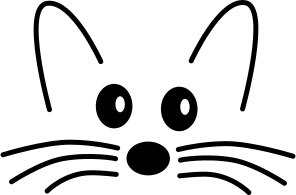
\includegraphics[width=1.4em]{squeak-logo}}}
\iftoshelse{
	\usepackage{marginnote}
		\renewcommand*{\marginfont}{\footnotesize}
	\newcommand{\vartriangleout}{\ifthenelse{\isodd{\thepage}}{\vartriangleright}{\vartriangleleft}}
	\newcommand{\dothisicon}{\fcolorbox{blue!65}{white}{\highlight{$\vartriangleout$}}}
	\newcommand{\dothis}[1]{%
		\noindent\par\noindent
		{\reversemarginpar
			\marginnote{\fcolorbox{blue!65}{white}{\highlight{$\vartriangleout$}}}}
		%\MarginLabel{do this}
		\noindent\emph{#1}
		\nopagebreak}
}{
	\newcommand{\dothisicon}{\raisebox{-.5ex}{
\includegraphics[height=1.2em]{pharo}}}
	\newcommand{\dothis}[1]{%
		\medskip
		\noindent\dothisicon
		\ifx#1\empty\else\quad\emph{#1}\fi
		\par\smallskip\nopagebreak}
}
%===> NEW VERSION <===
% NB: To use this in an individual chapter, you must set:
%\graphicspath{{figures/} {../figures/}}
% at the head of the chapter.  Don't forget the final /
%=============================================================
%:Reader hints (hint)
%
% Indicates a non-obvious consequence
\newcommand{\hint}[1]{\vspace{1ex}\noindent\fbox{\textsc{Hint}} \emph{#1}}
%=================================================================
% graphics for Morphic handles
\newcommand{\grabHandle}{\raisebox{-0.2ex}{
\includegraphics[width=1em]{blackHandle}}}
\newcommand{\moveHandle}{\raisebox{-0.2ex}{
\includegraphics[width=1em]{moveHandle}}}
\newcommand{\debugHandle}{\raisebox{-0.2ex}{
\includegraphics[width=1em]{debugHandle}}}
%=============================================================
%:Highlighting Important stuff (doublebox)
%
% From Seaside book ...
\newsavebox{\SavedText}
\newlength{\InnerBoxRule}\setlength{\InnerBoxRule}{.75\fboxrule}
\newlength{\OuterBoxRule}\setlength{\OuterBoxRule}{1.5\fboxrule}
\newlength{\BoxSeparation}\setlength{\BoxSeparation}{1.5\fboxrule}
\addtolength{\BoxSeparation}{.5pt}
\newlength{\SaveBoxSep}\setlength{\SaveBoxSep}{2\fboxsep}
%
\newenvironment{doublebox}{\begin{lrbox}{\SavedText}
    \begin{minipage}{.75\textwidth}}
    {\end{minipage}\end{lrbox}\begin{center}
    \setlength{\fboxsep}{\BoxSeparation}\setlength{\fboxrule}{\OuterBoxRule}
    \fbox{\setlength{\fboxsep}{\SaveBoxSep}\setlength{\fboxrule}{\InnerBoxRule}%
      \fbox{\usebox{\SavedText}}}
  \end{center}}
% Use this:
\newcommand{\important}[1]{\begin{doublebox}#1\end{doublebox}}
%=============================================================
%:Section depth
\setcounter{secnumdepth}{2}
%% for this to happen start the file with
%\ifx\wholebook\relax\else
%% $Author$
% $Date$
% $Revision$

% HISTORY:
% 2006-10-31 - Oscar code macros
% ...

%=============================================================
% NB: documentclass must be set in main document.
% Allows book to be generated in multiple formats.
%=============================================================
%:Packages
\usepackage[T1]{fontenc}  %%%%%% really important to get the code directly in the text!
\usepackage{lmodern}
%\usepackage[scaled=0.85]{bookmanx} % needs another scale factor if used with \renewcommand{\sfdefault}{cmbr}
\usepackage{palatino}
\usepackage[scaled=0.85]{helvet}
\usepackage[protrusion,expansion=false]{microtype}
\usepackage{graphicx}
\usepackage{theorem}
\usepackage[english]{babel}
% ON: pdfsync breaks the use of p{width} for tabular columns!
\ifdefined\usepdfsync\usepackage{pdfsync}\fi % Requires texlive 2007
%=============================================================
%:More packages
%Stef should check which ones are used!
%\usepackage{picinpar}
%\usepackage{layout}
%\usepackage{color}
%\usepackage{enum}
%\usepackage{a4wide}
% \usepackage{fancyhdr}
\usepackage{ifthen}
\usepackage{float}
\usepackage{longtable}
\usepackage{makeidx}
\usepackage[nottoc]{tocbibind}
\usepackage{multicol}
\usepackage{booktabs}	% book-style tables
\usepackage{topcapt}	% enables \topcaption
\usepackage{multirow}
\usepackage{tabularx}
%\usepackage[bottom]{footmisc}
\usepackage{xspace}
\usepackage{alltt}
\usepackage{amssymb,textcomp}
\usepackage[usenames,dvipsnames]{color}
%\usepackage{colortbl}
\usepackage[hang]{subfigure}\makeatletter\def\p@subfigure{\thefigure\,}\makeatother
\usepackage{rotating}
\usepackage{enumitem}	% apb: allows more control over tags in enumerations
\usepackage{verbatim}     % for comment environment
\usepackage{varioref}	% for page references that work
\labelformat{footnote}{\thechapter--#1} % to distinguish citations from jurabib
\usepackage{needspace}
\usepackage{isodateo} % enable \isodate
\usepackage[newparttoc,pagestyles]{titlesec}
\usepackage{titletoc}
\usepackage{wrapfig}

\usepackage[
	super,
	citefull=first,
	authorformat={allreversed,and},
	titleformat={commasep,italic}
]{jurabib} % citations as footnotes
\usepackage[
	colorlinks=true,
	linkcolor=black,
	urlcolor=black,
	citecolor=black
]{hyperref}   % should come last
%=============================================================
%:PDF version
\pdfminorversion=3 % Set PDF to 1.3 for Lulu
%=============================================================
%:URL style
\makeatletter
\def\url@leostyle{%
  \@ifundefined{selectfont}{\def\UrlFont{\sf}}{\def\UrlFont{\sffamily}}}
\makeatother
% Now actually use the newly defined style.
\urlstyle{leo}
%=============================================================
%:Booleans
\newboolean{lulu}
\setboolean{lulu}{false}
\newcommand{\ifluluelse}[2]{\ifthenelse{\boolean{lulu}}{#1}{#2}}
%=============================================================
%:Names
\newcommand{\SUnit}{SUnit\xspace}
\newcommand{\sunit}{SUnit\xspace}
\newcommand{\xUnit}{$x$Unit\xspace}
\newcommand{\JUnit}{JUnit\xspace}
\newcommand{\st}{Smalltalk\xspace}
\newcommand{\pharo}{Pharo\xspace} % Use this, not \Pharo
%\newcommand{\sqmap}{SqueakMap\xspace}
\newcommand{\squeak}{Squeak\xspace} % use this, not \Squeak or \sq
\newcommand{\sqsrc}{SqueakSource\xspace}
\newcommand{\sbe}{\url{http://SqueakByExample.org}\xspace}
\newcommand{\pharoweb}{\url{http://pharo-project.org}\xspace}
\newcommand{\pbe}{\url{http://PharoByExample.org}\xspace}
\newcommand{\sba}{\url{http://SquareBracketAssociates.org}\xspace}
\newcommand{\bam}{\lct{Bounc\-ing\-Atoms\-Morph}\xspace}
%=============================================================
%:Markup macros for proof-reading
\usepackage[normalem]{ulem} % for \sout
\usepackage{xcolor}
\newcommand{\ra}{$\rightarrow$}
\newcommand{\ugh}[1]{\textcolor{red}{\uwave{#1}}} % please rephrase
\newcommand{\ins}[1]{\textcolor{blue}{\uline{#1}}} % please insert
\newcommand{\del}[1]{\textcolor{red}{\sout{#1}}} % please delete
\newcommand{\chg}[2]{\textcolor{red}{\sout{#1}}{\ra}\textcolor{blue}{\uline{#2}}} % please change
%=============================================================
%:Editorial comment macros
%\newcommand{\nnbb}[2]{
%    % \fbox{\bfseries\sffamily\scriptsize#1}
%    \fcolorbox{gray}{yellow}{\bfseries\sffamily\scriptsize#1}
%    {\sf\small$\blacktriangleright$\textit{#2}$\blacktriangleleft$}
%   }
\newcommand{\yellowbox}[1]{\fcolorbox{gray}{yellow}{\bfseries\sffamily\scriptsize#1}}
\newcommand{\triangles}[1]{{\sf\small$\blacktriangleright$\textit{#1}$\blacktriangleleft$}}
\newcommand{\nnbb}[2]{\yellowbox{#1} \triangles{#2}}
\newcommand{\fix}{\yellowbox{FIX!}}
\newcommand{\here}{\yellowbox{CONTINUE HERE!}}
% editor macros
\newcommand{\apl}[1]{\nnbb{Alain}{#1}} % Alain
\newcommand{\ab}[1]{\nnbb{Andrew}{#1}} % Black
\newcommand{\sd}[1]{\nnbb{St\'{e}f}{#1}} % Ducasse
\newcommand{\gl}[1]{\nnbb{Guillaume}{#1}} % Ducasse
\newcommand{\cd}[1]{\nnbb{Christophe}{#1}} % Ducasse
\newcommand{\sig}[1]{\nnbb{Igor}{#1}} % Igor
\newcommand{\dc}[1]{\nnbb{DamienC}{#1}} % Ducasse
\newcommand{\md}[1]{\nnbb{Marcus}{#1}} % Denker
\newcommand{\on}[1]{\nnbb{Oscar}{#1}} % Nierstrasz
\newcommand{\damien}[1]{\nnbb{Damien}{#1}} % Pollet
\newcommand{\lr}[1]{\nnbb{Lukas}{#1}} % Renggli
\newcommand{\orla}[1]{\nnbb{Orla}{#1}} % Greevy
\newcommand{\alex}[1]{\nnbb{Alex}{#1}} % Bergel
\newcommand{\alx}[1]{\nnbb{Alex}{#1}} % Bergel
\newcommand{\dr}[1]{\nnbb{David}{#1}} % Roethlisberger
\newcommand{\ja}[1]{\nnbb{Jannik}{#1}} % Laval
\newcommand{\cb}[1]{\nnbb{Camillo}{#1}} % Bruni
\newcommand{\jr}[1]{\nnbb{Jorge}{#1}} % Ressia
\newcommand{\jb}[1]{\nnbb{JB}{#1}} % JB
\newcommand{\jp}[1]{\nnbb{Javier}{#1}} % Pimas
\newcommand{\fp}[1]{\nnbb{Fabrizio}{#1}} % Perin
\newcommand{\michael}[1]{\nnbb{Michael}{#1}} % Davies
\newcommand{\ew}[1]{\nnbb{Erwann}{#1}} % Wernli
\newcommand{\mb}[1]{\nnbb{Martial}{#1}} % Boniou
\newcommand{\hw}[1]{\nnbb{Hernan}{#1}} % Wilkinson
\newcommand{\ben}[1]{\nnbb{Benjamin}{#1}} % Benjamin Van Ryseghem
\newcommand{\hjo}[1]{\nnbb{HwaJong}{#1}} % HwaJong Oh aka daliot
\newcommand{\ml}[1]{\nnbb{Max}{#1}} % Max Leske
\newcommand{\mmp}[1]{\nnbb{Mariano}{#1}} % Mariano Martinez Peck
\newcommand{\luc}[1]{\nnbb{Luc}{#1}} % Luc Fabresse
\newcommand{\dkl}[1]{\nnbb{Daniel}{#1}} % Daniel Lyons
\newcommand{\vu}[1]{\nnbb{Veronica}{#1}} % Veronica Uquillas Gomez
\newcommand{\martin}[1]{\nnbb{Martin}{#1}} % Martin Dias
\newcommand{\vp}[1]{\nnbb{Vanessa}{#1}} % Vanessa Pena
\newcommand{\gp}[1]{\nnbb{Guille}{#1}} % Guillermo Polito

%=============================================================
%:Abbreviation macros
\newcommand{\ie}{\emph{i.e.},\xspace}
\newcommand{\eg}{\emph{e.g.},\xspace}
\newcommand{\etc}{etc.\xspace}
%=============================================================
%:Cross reference macros
\newcommand{\charef}[1]{Chapter~\ref{cha:#1}\xspace}
\newcommand{\secref}[1]{Section~\ref{sec:#1}\xspace}
\newcommand{\figref}[1]{Figure~\ref{fig:#1}\xspace}
\newcommand{\Figref}[1]{Figure~\ref{fig:#1}\xspace}
\newcommand{\appref}[1]{Appendix~\ref{app:#1}\xspace}
\newcommand{\tabref}[1]{Table~\ref{tab:#1}\xspace}
\newcommand{\faqref}[1]{FAQ~\ref{faq:#1}, p.~\pageref{faq:#1}\xspace}
% APB: I removed trailing \xspace commands from these macros because
% \xspace mostly doesn't work.  If you want a space after your
% references, type one!
% ON: xspace has always worked just fine for me!  Please leave them in.
%
\newcommand{\ruleref}[1]{\ref{rule:#1}\xspace}
%
\newcommand{\egref}[1]{example~\ref{eg:#1}\xspace}
\newcommand{\Egref}[1]{Example~\ref{eg:#1}\xspace}
%
\newcommand{\scrref}[1]{script~\ref{scr:#1}\xspace}
\newcommand{\Scrref}[1]{Script~\ref{scr:#1}\xspace}
\newcommand{\tscrref}[1]{the script~\ref{scr:#1}\xspace}
\newcommand{\Tscrref}[1]{The script~\ref{scr:#1}\xspace}
%
\newcommand{\mthref}[1]{method~\ref{mth:#1}\xspace}
\newcommand{\mthsref}[1]{methods~\ref{mth:#1}\xspace}
\newcommand{\Mthref}[1]{Method~\ref{mth:#1}\xspace}
\newcommand{\tmthref}[1]{the method~\ref{mth:#1}\xspace}
\newcommand{\Tmthref}[1]{The method~\ref{mth:#1}\xspace}
%
\newcommand{\clsref}[1]{class~\ref{cls:#1}\xspace}
\newcommand{\tclsref}[1]{the class~\ref{cls:#1}\xspace}
\newcommand{\Tclsref}[1]{The class~\ref{cls:#1}\xspace}

\newcommand{\chalabel}[1]{\label{cha:#1}}
\newcommand{\seclabel}[1]{\label{sec:#1}}
\newcommand{\figlabel}[1]{\label{fig:#1}}
\newcommand{\tablabel}[1]{\label{tab:#1}}
\newcommand{\rulelabel}[1]{\label{rule:#1}}
\newcommand{\eglabel}[1]{\label{eg:#1}}
\newcommand{\scrlabel}[1]{\label{scr:#1}}
\newcommand{\mthlabel}[1]{\label{mth:#1}}
\newcommand{\clslabel}[1]{\label{cls:#1}}
\newcommand{\faqlabel}[1]{\label{faq:#1}}
%=============================================================
%:Menu item macro
% for menu items, so we can change our minds on how to print them! (apb)
\definecolor{lightgray}{gray}{0.89}
\newcommand{\menu}[1]{{%
	\setlength{\fboxsep}{0pt}%
	\colorbox{lightgray}{{{\upshape\sffamily\strut \,#1\,}}}}}
\newcommand{\link}[1]{{%
	\fontfamily{lmr}\selectfont
 	\upshape{\sffamily \underline{#1}}}}
% For submenu items:
\newcommand{\go}{\,$\triangleright$\,}
% \newcommand{\go}{\,$\blacktriangleright$\,}
% For keyboard shortcuts:
%\newcommand{\short}[1]{\mbox{$\langle${\sc CMD}$\rangle$-#1}\xspace}
\newcommand{\short}[1]{\mbox{{\sc cmd}\hspace{0.08em}--\hspace{0.09em}#1}\xspace}
% For buttons:
\newcommand{\button}[1]{{%
	\setlength{\fboxsep}{0pt}%
	\fbox{{\upshape\sffamily\strut \,#1\,}}}}
% NB: The button macro does not work within captions -- incompatible with xcolor package :-(
\newcommand{\toolsflap}{\textit{Tools} flap\xspace}
%=============================================================
%:Mouse clicks
\newcommand{\click}{click\xspace} % RED
\newcommand{\actclick}{action-click\xspace} % YELLOW
\newcommand{\metaclick}{meta-click\xspace} % BLUE
\newcommand{\Click}{Click\xspace} % RED
\newcommand{\Actclick}{Action-click\xspace} % YELLOW
\newcommand{\Metaclick}{Meta-click\xspace} % BLUE
%=============================================================
%:ToSh macros
\newboolean{tosh}
\setboolean{tosh}{false}
\newcommand{\iftoshelse}[2]{\ifthenelse{\boolean{tosh}}{#1}{#2}}
%=============================================================
%:ToSh colors
%\newcommand{\highlightcolor}{\color{blue!65}}
%\newcommand{\boxcolor}{\color{gray!25}}
\newcommand{\highlight}[1]{\textcolor{blue!65}{#1}}
%\newcommand{\codecolor}{\color{blue!65}}
%%\setlength{\fboxrule}{2pt}
%\newcommand{\asPict}[1]{%
%	{\Large\highlight{#1}}}
%=============================================================
%:Reader cues (do this)
%
% Indicate something the reader should try out.
% \newcommand{\dothisicon}{\raisebox{-.5ex}{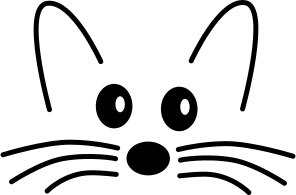
\includegraphics[width=1.4em]{squeak-logo}}}
\iftoshelse{
	\usepackage{marginnote}
		\renewcommand*{\marginfont}{\footnotesize}
	\newcommand{\vartriangleout}{\ifthenelse{\isodd{\thepage}}{\vartriangleright}{\vartriangleleft}}
	\newcommand{\dothisicon}{\fcolorbox{blue!65}{white}{\highlight{$\vartriangleout$}}}
	\newcommand{\dothis}[1]{%
		\noindent\par\noindent
		{\reversemarginpar
			\marginnote{\fcolorbox{blue!65}{white}{\highlight{$\vartriangleout$}}}}
		%\MarginLabel{do this}
		\noindent\emph{#1}
		\nopagebreak}
}{
	\newcommand{\dothisicon}{\raisebox{-.5ex}{
\includegraphics[height=1.2em]{pharo}}}
	\newcommand{\dothis}[1]{%
		\medskip
		\noindent\dothisicon
		\ifx#1\empty\else\quad\emph{#1}\fi
		\par\smallskip\nopagebreak}
}
%===> NEW VERSION <===
% NB: To use this in an individual chapter, you must set:
%\graphicspath{{figures/} {../figures/}}
% at the head of the chapter.  Don't forget the final /
%=============================================================
%:Reader hints (hint)
%
% Indicates a non-obvious consequence
\newcommand{\hint}[1]{\vspace{1ex}\noindent\fbox{\textsc{Hint}} \emph{#1}}
%=================================================================
% graphics for Morphic handles
\newcommand{\grabHandle}{\raisebox{-0.2ex}{
\includegraphics[width=1em]{blackHandle}}}
\newcommand{\moveHandle}{\raisebox{-0.2ex}{
\includegraphics[width=1em]{moveHandle}}}
\newcommand{\debugHandle}{\raisebox{-0.2ex}{
\includegraphics[width=1em]{debugHandle}}}
%=============================================================
%:Highlighting Important stuff (doublebox)
%
% From Seaside book ...
\newsavebox{\SavedText}
\newlength{\InnerBoxRule}\setlength{\InnerBoxRule}{.75\fboxrule}
\newlength{\OuterBoxRule}\setlength{\OuterBoxRule}{1.5\fboxrule}
\newlength{\BoxSeparation}\setlength{\BoxSeparation}{1.5\fboxrule}
\addtolength{\BoxSeparation}{.5pt}
\newlength{\SaveBoxSep}\setlength{\SaveBoxSep}{2\fboxsep}
%
\newenvironment{doublebox}{\begin{lrbox}{\SavedText}
    \begin{minipage}{.75\textwidth}}
    {\end{minipage}\end{lrbox}\begin{center}
    \setlength{\fboxsep}{\BoxSeparation}\setlength{\fboxrule}{\OuterBoxRule}
    \fbox{\setlength{\fboxsep}{\SaveBoxSep}\setlength{\fboxrule}{\InnerBoxRule}%
      \fbox{\usebox{\SavedText}}}
  \end{center}}
% Use this:
\newcommand{\important}[1]{\begin{doublebox}#1\end{doublebox}}
%=============================================================
%:Section depth
\setcounter{secnumdepth}{2}
%% for this to happen start the file with
%\ifx\wholebook\relax\else
%\input{../common.tex}
%\begin{document}
%\fi
% and terminate by
% \ifx\wholebook\relax\else\end{document}\fi

\DeclareGraphicsExtensions{.pdf, .jpg, .png}
%=============================================================
%:PDF setup
\hypersetup{
%   a4paper,
%   pdfstartview=FitV,
%   colorlinks,
%   linkcolor=darkblue,
%   citecolor=darkblue,
   pdftitle={Pharo by Example},
   pdfauthor={Andrew P. Black, St\'ephane Ducasse,	Oscar Nierstrasz,
Damien Pollet},
   pdfkeywords={Smalltalk, Squeak, Object-Oriented Programming, OOP},
   pdfsubject={Computer Science}
}
%=============================================================
%:Page layout and appearance
%
% \renewcommand{\headrulewidth}{0pt}
\renewcommand{\chaptermark}[1]{\markboth{#1}{}}
\renewcommand{\sectionmark}[1]{\markright{\thesection\ #1}}
\renewpagestyle{plain}[\small\itshape]{%
	\setheadrule{0pt}%
	\sethead[][][]{}{}{}%
	\setfoot[][][]{}{}{}}
\renewpagestyle{headings}[\small\itshape]{%
	\setheadrule{0pt}%
	\setmarks{chapter}{section}%
	\sethead[\thepage][][\chaptertitle]{\sectiontitle}{}{\thepage}%
	\setfoot[][][]{}{}{}}
%=============================================================
%:Title section setup and TOC numbering depth
\setcounter{secnumdepth}{1}
\setcounter{tocdepth}{1}
\titleformat{\part}[display]{\centering}{\huge\partname\ \thepart}{1em}{\Huge\textbf}[]
\titleformat{\chapter}[display]{}{\huge\chaptertitlename\ \thechapter}{1em}{\Huge\raggedright\textbf}[]
\titlecontents{part}[3pc]{%
		\pagebreak[2]\addvspace{1em plus.4em minus.2em}%
		\leavevmode\large\bfseries}
	{\contentslabel{3pc}}{\hspace*{-3pc}}
	{}[\nopagebreak]
\titlecontents{chapter}[3pc]{%
		\pagebreak[0]\addvspace{1em plus.2em minus.2em}%
		\leavevmode\bfseries}
	{\contentslabel{3pc}}{}
	{\hfill\contentspage}[\nopagebreak]
\dottedcontents{section}[3pc]{}{3pc}{1pc}
\dottedcontents{subsection}[3pc]{}{0pc}{1pc}
% \dottedcontents{subsection}[4.5em]{}{0pt}{1pc}
% Make \cleardoublepage insert really blank pages http://www.tex.ac.uk/cgi-bin/texfaq2html?label=reallyblank
\let\origdoublepage\cleardoublepage
\newcommand{\clearemptydoublepage}{%
  \clearpage
  {\pagestyle{empty}\origdoublepage}}
\let\cleardoublepage\clearemptydoublepage % see http://www.tex.ac.uk/cgi-bin/texfaq2html?label=patch
%=============================================================
%:FAQ macros (for FAQ chapter)
\newtheorem{faq}{FAQ}
\newcommand{\answer}{\paragraph{Answer}\ }
%=============================================================
%:Listings package configuration
% \newcommand{\caret}{\makebox{\raisebox{0.4ex}{\footnotesize{$\wedge$}}}}
\newcommand{\caret}{\^\,}
\newcommand{\escape}{{\sf \textbackslash}}
\definecolor{source}{gray}{0.95}
\usepackage{listings}
\lstdefinelanguage{Smalltalk}{
%  morekeywords={self,super,true,false,nil,thisContext}, % This is overkill
  morestring=[d]',
  morecomment=[s]{"}{"},
  alsoletter={\#:},
  escapechar={!},
  literate=
    {BANG}{!}1
    {CARET}{\^}1
    {UNDERSCORE}{\_}1
    {\\st}{Smalltalk}9 % convenience -- in case \st occurs in code
    % {'}{{\textquotesingle}}1 % replaced by upquote=true in \lstset
    %{_}{{$\leftarrow$}}1
    {>>>}{{\sep}}1
    %{^}{{$\uparrow$}}1
    {~}{{$\sim$}}1
    {-}{{\texttt{-}}}1 %{\textminus}}1 %{-}{\hspace{-0.13em}}{-}}1  % the goal is to make - the same width as +
    % {+}{\sf+}1 %{\raisebox{0.08ex}{+}}}1      % and to raise + off the baseline to match -
    {-->}{{\quad$\longrightarrow$\quad}}3
    {~->}{{\quad$\leadsto$\quad}}3
	, % Don't forget the comma at the end!
  tabsize=4
}[keywords,comments,strings]

\lstset{language=Smalltalk,
	basicstyle=\sffamily,
	keywordstyle=\color{black}\bfseries,
	% stringstyle=\ttfamily, % Ugly! do we really want this? -- on
	mathescape=true,
	showstringspaces=false,
	keepspaces=true,
	breaklines=true,
	breakautoindent=true,
	backgroundcolor=\color{source},
	lineskip={-1pt}, % Ugly hack
	upquote=true, % straight quote; requires textcomp package
	columns=fullflexible} % no fixed width fonts
% In-line code (literal)
% Normally use this for all in-line code:

\newcommand{\ct}{\lstinline[mathescape=false,backgroundcolor=\color{white},basicstyle={\sffamily\upshape}]}
\newcommand{\cts}[1]{{\sffamily{\upshape{#1}}\xspace}}
% apb 2007.8.28 added the \upshape declaration to avoid getting italicized code in \dothis{ } sections.
% In-line code (latex enabled)
% Use this only in special situations where \ct does not work
% (within section headings ...):
\newcommand{\lct}[1]{{\textsf{\textup{#1}}}}
% Use these for system categories and protocols:
\newcommand{\scat}[1]{\emph{\textsf{#1}}\xspace}
\newcommand{\pkg}[1]{\emph{\textsf{#1}}\xspace}
\newcommand{\prot}[1]{\emph{\textsf{#1}}\xspace}
% Code environments
% NB: the arg is for tests
% Only code and example environments may be tests
\lstnewenvironment{code}[1]{%
	\lstset{%
		% frame=lines,
		frame=single,
		framerule=0pt,
		mathescape=false
	}
}{}
\def\ignoredollar#1{}
%=============================================================
%:Code environments (method, script ...)
% NB: the third arg is for tests
% Only code and example environments may be tests
\lstnewenvironment{example}[3][defaultlabel]{%
	\renewcommand{\lstlistingname}{Example}%
	\lstset{
		% frame=lines,
		frame=single,
		framerule=0pt,
		mathescape=false,
		caption={\emph{#2}},
		label={eg:#1}
	}
}{}
\lstnewenvironment{script}[2][defaultlabel]{%
\renewcommand{\lstlistingname}{Script}%
	\lstset{
		% frame=lines,
		frame=single,
		framerule=0pt,
		mathescape=false,
		name={Script},
		caption={\emph{#2}},
		label={scr:#1}
	}
}{}
\lstnewenvironment{method}[2][defaultlabel]{%
	\renewcommand{\lstlistingname}{Method}%
	\lstset{
		% frame=lines,
		frame=single,
		framerule=0pt,
		mathescape=false,
		name={Method},
		caption={\emph{#2}},
		label={mth:#1}
	}
}{}
\lstnewenvironment{methods}[2][defaultlabel]{% just for multiple methods at once
	\renewcommand{\lstlistingname}{Methods}%
	\lstset{
		% frame=lines,
		frame=single,
		framerule=0pt,
		mathescape=false,
		name={Method},
		caption={\emph{#2}},
		label={mth:#1}
	}
}{}
\lstnewenvironment{numMethod}[2][defaultlabel]{%
	\renewcommand{\lstlistingname}{Method}%
	\lstset{
		numbers=left,
		numberstyle={\tiny\sffamily},
		% frame=lines,
		frame=single,
		framerule=0pt,
		mathescape=false,
		name={Method},
		caption={\emph{#2}},
		label={mth:#1}
	}
}{}
\lstnewenvironment{classdef}[2][defaultlabel]{%
	\renewcommand{\lstlistingname}{Class}%
	\lstset{
		% frame=lines,
		frame=single,
		framerule=0pt,
		mathescape=false,
		name={Class},
		caption={\emph{#2}},
		label={cls:#1}
	}
}{}
%=============================================================
%:Reserving space
% Usually need one more line than the actual lines of code
\newcommand{\needlines}[1]{\Needspace{#1\baselineskip}}
%=============================================================
%:Indexing macros
% Macros ending with "ind" generate text as well as an index entry
% Macros ending with "index" *only* generate an index entry
\newcommand{\ind}[1]{\index{#1}#1\xspace} % plain text
\newcommand{\subind}[2]{\index{#1!#2}#2\xspace} % show #2, subindex under #1
\newcommand{\emphind}[1]{\index{#1}\emph{#1}\xspace} % emph #1
\newcommand{\emphsubind}[2]{\index{#1!#2}\emph{#2}\xspace} % show emph #2, subindex inder #1
\newcommand{\scatind}[1]{\index{#1@\textsf{#1} (category)}\scat{#1}} % category
\newcommand{\pkgind}[1]{\index{#1@\textsf{#1} (package)}\pkg{#1}} % package
\newcommand{\protind}[1]{\index{#1@\textsf{#1} (protocol)}\prot{#1}} % protocol
\newcommand{\clsind}[1]{\index{#1@\textsf{#1} (class)}\ct{#1}\xspace}
% \newcommand{\clsind}[1]{\index{#1!\#@(class)}\ct{#1}\xspace} % class
\newcommand{\clsindplural}[1]{\index{#1!\#@(class)}\ct{#1}s\xspace} % class
\newcommand{\cvind}[1]{\index{#1@\textsf{#1} (class variable)}\ct{#1}\xspace} % class var
\newcommand{\glbind}[1]{\index{#1@\textsf{#1} (global)}\ct{#1}\xspace} % global
\newcommand{\patind}[1]{\index{#1@#1 (pattern)}\ct{#1}\xspace} % pattern
\newcommand{\pvind}[1]{\index{#1@\textsf{#1} (pseudo variable)}\ct{#1}\xspace} % pseudo var
\newcommand{\clsmthind}[2]{\index{#1!#2@\ct{#2}}\ct{#1>>>#2}\xspace} % class + method name
\newcommand{\mthind}[2]{\index{#1!#2@\ct{#2}}\ct{#2}\xspace} % show method name only
\newcommand{\lmthind}[2]{\index{#1!#2@\ct{#2}}\lct{#2}\xspace} % show method name only
\newcommand{\cmind}[2]{\index{#1!#2@\ct{#2}}\ct{#1>>>#2}\xspace} % show class>>method
\newcommand{\lcmind}[2]{\index{#1!#2@\ct{#2}}\lct{#1>>>#2}\xspace} % show class>>method
\newcommand{\toolsflapind}{\index{Tools flap}\toolsflap} % index tools flap
% The following only generate an index entry:
% \newcommand{\clsindex}[1]{\index{#1@\textsf{#1} (class)}}
\newcommand{\clsindex}[1]{\index{#1!\#@(class)}} % class
\newcommand{\mthindex}[2]{\index{#1!#2@\ct{#2}}} % method
\newcommand{\cmindex}[2]{\index{#1!#2@\ct{#2}}} % class>>method
\newcommand{\cvindex}[1]{\index{#1@\textsf{#1} (class variable)}} % class var
\newcommand{\glbindex}[1]{\index{#1@\textsf{#1} (global)}}% global
\newcommand{\pvindex}[1]{\index{#1@\textsf{#1} (pseudo variable)}}% pseudo var
\newcommand{\seeindex}[2]{\index{#1|see{#2}}} % #1, see #2
\newcommand{\scatindex}[1]{\index{#1@\textsf{#1} (category)}} % category
\newcommand{\pkgindex}[1]{\index{#1@\textsf{#1} (package)}} % package
\newcommand{\protindex}[1]{\index{#1@\textsf{#1} (protocol)}} % protocol
% How can we have the main entry page numbers in bold yet not break the hyperlink?
\newcommand{\boldidx}[1]{{\bf #1}} % breaks hyperlink
%\newcommand{\indmain}[1]{\index{#1|boldidx}#1\xspace} % plain text, main entry
%\newcommand{\emphsubindmain}[2]{\index{#1!#2|boldidx}\emph{#2}\xspace} % subindex, main entry
%\newcommand{\subindmain}[2]{\index{#1!#2|boldidx}#2\xspace} % subindex, main entry
%\newcommand{\clsindmain}[1]{\index{#1@\textsf{#1} (class)|boldidx}\ct{#1}\xspace}
%\newcommand{\clsindmain}[1]{\index{#1!\#@(class)|boldidx}\ct{#1}\xspace} % class main
%\newcommand{\indexmain}[1]{\index{#1|boldidx}} % main index entry only
\newcommand{\indmain}[1]{\index{#1}#1\xspace} % The main index entry for this item
\newcommand{\emphsubindmain}[2]{\index{#1!#2}\emph{#2}\xspace} % subindex, main entry
\newcommand{\subindmain}[2]{\index{#1!#2}#2\xspace} % subindex, main entry
%\newcommand{\clsindmain}[1]{\index{#1@\textsf{#1} (class)}\ct{#1}\xspace}
\newcommand{\clsindmain}[1]{\index{#1!\#@(class)}\ct{#1}\xspace} % class main
\newcommand{\clsindexmain}[1]{\index{#1!\#@(class)}} % class main index only
\newcommand{\indexmain}[1]{\index{#1}}
%=============================================================
%:Code macros
% some constants
\newcommand{\codesize}{\small}
\newcommand{\codefont}{\sffamily}
%\newcommand{\cat}[1]{\textit{In category #1}}%%To remove later
\newlength{\scriptindent}
\setlength{\scriptindent}{.3cm}
%% Method presentation constants
\newlength{\methodindent}
\newlength{\methodwordlength}
\newlength{\aftermethod}
\setlength{\methodindent}{0.2cm}
\settowidth{\methodwordlength}{\ M\'ethode\ }
%=============================================================
%:Smalltalk macros
%\newcommand{\sep}{{$\gg$}}
\newcommand{\sep}{\mbox{>>}}
\newcommand{\self}{\lct{self}\xspace}
\newcommand{\super}{\lct{super}\xspace}
\newcommand{\nil}{\lct{nil}\xspace}
%=============================================================
% be less conservative about float placement
% these commands are from http://www.tex.ac.uk/cgi-bin/texfaq2html?label=floats
\renewcommand{\topfraction}{.9}
\renewcommand{\bottomfraction}{.9}
\renewcommand{\textfraction}{.1}
\renewcommand{\floatpagefraction}{.85}
\renewcommand{\dbltopfraction}{.66}
\renewcommand{\dblfloatpagefraction}{.85}
\setcounter{topnumber}{9}
\setcounter{bottomnumber}{9}
\setcounter{totalnumber}{20}
\setcounter{dbltopnumber}{9}
%=============================================================
% Give information from each chapter's author
\newcommand{\contact}[2]{\textbf{#1} \textsf{(#2)}}

\newcommand{\chapterauthor}[1]{\emph{with the participation of:\\#1}\\}
\newcommand{\chapterwritten}[1]{\emph{written by:\\#1}\\}

\newcommand{\authornoury}{\contact{Noury Bouraqadi}{Noury.Bouraqadi@mines-douai.fr}}
\newcommand{\authorluc}{\contact{Luc Fabresse}{Luc.Fabresse@mines-douai.fr}}
\newcommand{\authordamienc}{\contact{Damien Cassou}{damien.cassou@gmail.com}}
\newcommand{\authoroscar}{\contact{Oscar Nierstrasz}{oscar.nierstrasz@acm.org}}
\newcommand{\authorsteph}{\contact{St\'ephane Ducasse}{stephane.ducasse@inria.fr}}
\newcommand{\authoralex}{\contact{Alexandre Bergel}{alexandre@bergel.eu}}
\newcommand{\authorolivier}{\contact{Olivier Auverlot}{olivier.auverlot@inria.fr}}
\newcommand{\authornicolas}{\contact{Nicolas Cellier}{nicolas.cellier.aka.nice@gmail.com}}
\newcommand{\authormarcus}{\contact{Marcus Denker}{marcus.denker@inria.fr}}
\newcommand{\authoralain}{\contact{Alain Plantec}{alain.plantec@univ-brest.fr}}
\newcommand{\authordale}{\contact{Dale Henrichs}{dale.henrichs@gemstone.com}}
\newcommand{\authormariano}{\contact{Mariano Martinez Peck}{marianopeck@gmail.com}}
\newcommand{\authorsven}{\contact{Sven Van Caekenberghe}{sven@beta9.be}}
\newcommand{\authorlukas}{\contact{Lukas Renggli}{renggli@gmail.com}}
\newcommand{\authorjankurs}{\contact{Jan Kurs}{kurs@iam.unibe.ch}}
\newcommand{\authorguillaume}{\contact{Guillaume Larcheveque}{guillaume.larcheveque@gmail.com}}
\newcommand{\authorguillep}{\contact{Guillermo Polito}{guillermopolito@gmail.com}}
\newcommand{\authorclement}{\contact{Cl\'ement Bera}{bera.clement@gmail.com}}
\newcommand{\authormax}{\contact{Max Leske}{maxleske@gmail.com}}
\newcommand{\authorvanessa}{\contact{Vanessa Pe\~{n}a-Araya}{van.c.pena@gmail.com}}
\newcommand{\authorcamillo}{\contact{Camillo Bruni}{camillobruni@gmail.com}}

%=============================================================
% apb doesn't like paragraphs to run in to each other without a break
\parskip 1ex
%=============================================================
%:Stuff to check, merge or deprecate
%\setlength{\marginparsep}{2mm}
%\renewcommand{\baselinestretch}{1.1}
%=============================================================
\usepackage{tikz}

%\begin{document}
%\fi
% and terminate by
% \ifx\wholebook\relax\else\end{document}\fi

\DeclareGraphicsExtensions{.pdf, .jpg, .png}
%=============================================================
%:PDF setup
\hypersetup{
%   a4paper,
%   pdfstartview=FitV,
%   colorlinks,
%   linkcolor=darkblue,
%   citecolor=darkblue,
   pdftitle={Pharo by Example},
   pdfauthor={Andrew P. Black, St\'ephane Ducasse,	Oscar Nierstrasz,
Damien Pollet},
   pdfkeywords={Smalltalk, Squeak, Object-Oriented Programming, OOP},
   pdfsubject={Computer Science}
}
%=============================================================
%:Page layout and appearance
%
% \renewcommand{\headrulewidth}{0pt}
\renewcommand{\chaptermark}[1]{\markboth{#1}{}}
\renewcommand{\sectionmark}[1]{\markright{\thesection\ #1}}
\renewpagestyle{plain}[\small\itshape]{%
	\setheadrule{0pt}%
	\sethead[][][]{}{}{}%
	\setfoot[][][]{}{}{}}
\renewpagestyle{headings}[\small\itshape]{%
	\setheadrule{0pt}%
	\setmarks{chapter}{section}%
	\sethead[\thepage][][\chaptertitle]{\sectiontitle}{}{\thepage}%
	\setfoot[][][]{}{}{}}
%=============================================================
%:Title section setup and TOC numbering depth
\setcounter{secnumdepth}{1}
\setcounter{tocdepth}{1}
\titleformat{\part}[display]{\centering}{\huge\partname\ \thepart}{1em}{\Huge\textbf}[]
\titleformat{\chapter}[display]{}{\huge\chaptertitlename\ \thechapter}{1em}{\Huge\raggedright\textbf}[]
\titlecontents{part}[3pc]{%
		\pagebreak[2]\addvspace{1em plus.4em minus.2em}%
		\leavevmode\large\bfseries}
	{\contentslabel{3pc}}{\hspace*{-3pc}}
	{}[\nopagebreak]
\titlecontents{chapter}[3pc]{%
		\pagebreak[0]\addvspace{1em plus.2em minus.2em}%
		\leavevmode\bfseries}
	{\contentslabel{3pc}}{}
	{\hfill\contentspage}[\nopagebreak]
\dottedcontents{section}[3pc]{}{3pc}{1pc}
\dottedcontents{subsection}[3pc]{}{0pc}{1pc}
% \dottedcontents{subsection}[4.5em]{}{0pt}{1pc}
% Make \cleardoublepage insert really blank pages http://www.tex.ac.uk/cgi-bin/texfaq2html?label=reallyblank
\let\origdoublepage\cleardoublepage
\newcommand{\clearemptydoublepage}{%
  \clearpage
  {\pagestyle{empty}\origdoublepage}}
\let\cleardoublepage\clearemptydoublepage % see http://www.tex.ac.uk/cgi-bin/texfaq2html?label=patch
%=============================================================
%:FAQ macros (for FAQ chapter)
\newtheorem{faq}{FAQ}
\newcommand{\answer}{\paragraph{Answer}\ }
%=============================================================
%:Listings package configuration
% \newcommand{\caret}{\makebox{\raisebox{0.4ex}{\footnotesize{$\wedge$}}}}
\newcommand{\caret}{\^\,}
\newcommand{\escape}{{\sf \textbackslash}}
\definecolor{source}{gray}{0.95}
\usepackage{listings}
\lstdefinelanguage{Smalltalk}{
%  morekeywords={self,super,true,false,nil,thisContext}, % This is overkill
  morestring=[d]',
  morecomment=[s]{"}{"},
  alsoletter={\#:},
  escapechar={!},
  literate=
    {BANG}{!}1
    {CARET}{\^}1
    {UNDERSCORE}{\_}1
    {\\st}{Smalltalk}9 % convenience -- in case \st occurs in code
    % {'}{{\textquotesingle}}1 % replaced by upquote=true in \lstset
    %{_}{{$\leftarrow$}}1
    {>>>}{{\sep}}1
    %{^}{{$\uparrow$}}1
    {~}{{$\sim$}}1
    {-}{{\texttt{-}}}1 %{\textminus}}1 %{-}{\hspace{-0.13em}}{-}}1  % the goal is to make - the same width as +
    % {+}{\sf+}1 %{\raisebox{0.08ex}{+}}}1      % and to raise + off the baseline to match -
    {-->}{{\quad$\longrightarrow$\quad}}3
    {~->}{{\quad$\leadsto$\quad}}3
	, % Don't forget the comma at the end!
  tabsize=4
}[keywords,comments,strings]

\lstset{language=Smalltalk,
	basicstyle=\sffamily,
	keywordstyle=\color{black}\bfseries,
	% stringstyle=\ttfamily, % Ugly! do we really want this? -- on
	mathescape=true,
	showstringspaces=false,
	keepspaces=true,
	breaklines=true,
	breakautoindent=true,
	backgroundcolor=\color{source},
	lineskip={-1pt}, % Ugly hack
	upquote=true, % straight quote; requires textcomp package
	columns=fullflexible} % no fixed width fonts
% In-line code (literal)
% Normally use this for all in-line code:

\newcommand{\ct}{\lstinline[mathescape=false,backgroundcolor=\color{white},basicstyle={\sffamily\upshape}]}
\newcommand{\cts}[1]{{\sffamily{\upshape{#1}}\xspace}}
% apb 2007.8.28 added the \upshape declaration to avoid getting italicized code in \dothis{ } sections.
% In-line code (latex enabled)
% Use this only in special situations where \ct does not work
% (within section headings ...):
\newcommand{\lct}[1]{{\textsf{\textup{#1}}}}
% Use these for system categories and protocols:
\newcommand{\scat}[1]{\emph{\textsf{#1}}\xspace}
\newcommand{\pkg}[1]{\emph{\textsf{#1}}\xspace}
\newcommand{\prot}[1]{\emph{\textsf{#1}}\xspace}
% Code environments
% NB: the arg is for tests
% Only code and example environments may be tests
\lstnewenvironment{code}[1]{%
	\lstset{%
		% frame=lines,
		frame=single,
		framerule=0pt,
		mathescape=false
	}
}{}
\def\ignoredollar#1{}
%=============================================================
%:Code environments (method, script ...)
% NB: the third arg is for tests
% Only code and example environments may be tests
\lstnewenvironment{example}[3][defaultlabel]{%
	\renewcommand{\lstlistingname}{Example}%
	\lstset{
		% frame=lines,
		frame=single,
		framerule=0pt,
		mathescape=false,
		caption={\emph{#2}},
		label={eg:#1}
	}
}{}
\lstnewenvironment{script}[2][defaultlabel]{%
\renewcommand{\lstlistingname}{Script}%
	\lstset{
		% frame=lines,
		frame=single,
		framerule=0pt,
		mathescape=false,
		name={Script},
		caption={\emph{#2}},
		label={scr:#1}
	}
}{}
\lstnewenvironment{method}[2][defaultlabel]{%
	\renewcommand{\lstlistingname}{Method}%
	\lstset{
		% frame=lines,
		frame=single,
		framerule=0pt,
		mathescape=false,
		name={Method},
		caption={\emph{#2}},
		label={mth:#1}
	}
}{}
\lstnewenvironment{methods}[2][defaultlabel]{% just for multiple methods at once
	\renewcommand{\lstlistingname}{Methods}%
	\lstset{
		% frame=lines,
		frame=single,
		framerule=0pt,
		mathescape=false,
		name={Method},
		caption={\emph{#2}},
		label={mth:#1}
	}
}{}
\lstnewenvironment{numMethod}[2][defaultlabel]{%
	\renewcommand{\lstlistingname}{Method}%
	\lstset{
		numbers=left,
		numberstyle={\tiny\sffamily},
		% frame=lines,
		frame=single,
		framerule=0pt,
		mathescape=false,
		name={Method},
		caption={\emph{#2}},
		label={mth:#1}
	}
}{}
\lstnewenvironment{classdef}[2][defaultlabel]{%
	\renewcommand{\lstlistingname}{Class}%
	\lstset{
		% frame=lines,
		frame=single,
		framerule=0pt,
		mathescape=false,
		name={Class},
		caption={\emph{#2}},
		label={cls:#1}
	}
}{}
%=============================================================
%:Reserving space
% Usually need one more line than the actual lines of code
\newcommand{\needlines}[1]{\Needspace{#1\baselineskip}}
%=============================================================
%:Indexing macros
% Macros ending with "ind" generate text as well as an index entry
% Macros ending with "index" *only* generate an index entry
\newcommand{\ind}[1]{\index{#1}#1\xspace} % plain text
\newcommand{\subind}[2]{\index{#1!#2}#2\xspace} % show #2, subindex under #1
\newcommand{\emphind}[1]{\index{#1}\emph{#1}\xspace} % emph #1
\newcommand{\emphsubind}[2]{\index{#1!#2}\emph{#2}\xspace} % show emph #2, subindex inder #1
\newcommand{\scatind}[1]{\index{#1@\textsf{#1} (category)}\scat{#1}} % category
\newcommand{\pkgind}[1]{\index{#1@\textsf{#1} (package)}\pkg{#1}} % package
\newcommand{\protind}[1]{\index{#1@\textsf{#1} (protocol)}\prot{#1}} % protocol
\newcommand{\clsind}[1]{\index{#1@\textsf{#1} (class)}\ct{#1}\xspace}
% \newcommand{\clsind}[1]{\index{#1!\#@(class)}\ct{#1}\xspace} % class
\newcommand{\clsindplural}[1]{\index{#1!\#@(class)}\ct{#1}s\xspace} % class
\newcommand{\cvind}[1]{\index{#1@\textsf{#1} (class variable)}\ct{#1}\xspace} % class var
\newcommand{\glbind}[1]{\index{#1@\textsf{#1} (global)}\ct{#1}\xspace} % global
\newcommand{\patind}[1]{\index{#1@#1 (pattern)}\ct{#1}\xspace} % pattern
\newcommand{\pvind}[1]{\index{#1@\textsf{#1} (pseudo variable)}\ct{#1}\xspace} % pseudo var
\newcommand{\clsmthind}[2]{\index{#1!#2@\ct{#2}}\ct{#1>>>#2}\xspace} % class + method name
\newcommand{\mthind}[2]{\index{#1!#2@\ct{#2}}\ct{#2}\xspace} % show method name only
\newcommand{\lmthind}[2]{\index{#1!#2@\ct{#2}}\lct{#2}\xspace} % show method name only
\newcommand{\cmind}[2]{\index{#1!#2@\ct{#2}}\ct{#1>>>#2}\xspace} % show class>>method
\newcommand{\lcmind}[2]{\index{#1!#2@\ct{#2}}\lct{#1>>>#2}\xspace} % show class>>method
\newcommand{\toolsflapind}{\index{Tools flap}\toolsflap} % index tools flap
% The following only generate an index entry:
% \newcommand{\clsindex}[1]{\index{#1@\textsf{#1} (class)}}
\newcommand{\clsindex}[1]{\index{#1!\#@(class)}} % class
\newcommand{\mthindex}[2]{\index{#1!#2@\ct{#2}}} % method
\newcommand{\cmindex}[2]{\index{#1!#2@\ct{#2}}} % class>>method
\newcommand{\cvindex}[1]{\index{#1@\textsf{#1} (class variable)}} % class var
\newcommand{\glbindex}[1]{\index{#1@\textsf{#1} (global)}}% global
\newcommand{\pvindex}[1]{\index{#1@\textsf{#1} (pseudo variable)}}% pseudo var
\newcommand{\seeindex}[2]{\index{#1|see{#2}}} % #1, see #2
\newcommand{\scatindex}[1]{\index{#1@\textsf{#1} (category)}} % category
\newcommand{\pkgindex}[1]{\index{#1@\textsf{#1} (package)}} % package
\newcommand{\protindex}[1]{\index{#1@\textsf{#1} (protocol)}} % protocol
% How can we have the main entry page numbers in bold yet not break the hyperlink?
\newcommand{\boldidx}[1]{{\bf #1}} % breaks hyperlink
%\newcommand{\indmain}[1]{\index{#1|boldidx}#1\xspace} % plain text, main entry
%\newcommand{\emphsubindmain}[2]{\index{#1!#2|boldidx}\emph{#2}\xspace} % subindex, main entry
%\newcommand{\subindmain}[2]{\index{#1!#2|boldidx}#2\xspace} % subindex, main entry
%\newcommand{\clsindmain}[1]{\index{#1@\textsf{#1} (class)|boldidx}\ct{#1}\xspace}
%\newcommand{\clsindmain}[1]{\index{#1!\#@(class)|boldidx}\ct{#1}\xspace} % class main
%\newcommand{\indexmain}[1]{\index{#1|boldidx}} % main index entry only
\newcommand{\indmain}[1]{\index{#1}#1\xspace} % The main index entry for this item
\newcommand{\emphsubindmain}[2]{\index{#1!#2}\emph{#2}\xspace} % subindex, main entry
\newcommand{\subindmain}[2]{\index{#1!#2}#2\xspace} % subindex, main entry
%\newcommand{\clsindmain}[1]{\index{#1@\textsf{#1} (class)}\ct{#1}\xspace}
\newcommand{\clsindmain}[1]{\index{#1!\#@(class)}\ct{#1}\xspace} % class main
\newcommand{\clsindexmain}[1]{\index{#1!\#@(class)}} % class main index only
\newcommand{\indexmain}[1]{\index{#1}}
%=============================================================
%:Code macros
% some constants
\newcommand{\codesize}{\small}
\newcommand{\codefont}{\sffamily}
%\newcommand{\cat}[1]{\textit{In category #1}}%%To remove later
\newlength{\scriptindent}
\setlength{\scriptindent}{.3cm}
%% Method presentation constants
\newlength{\methodindent}
\newlength{\methodwordlength}
\newlength{\aftermethod}
\setlength{\methodindent}{0.2cm}
\settowidth{\methodwordlength}{\ M\'ethode\ }
%=============================================================
%:Smalltalk macros
%\newcommand{\sep}{{$\gg$}}
\newcommand{\sep}{\mbox{>>}}
\newcommand{\self}{\lct{self}\xspace}
\newcommand{\super}{\lct{super}\xspace}
\newcommand{\nil}{\lct{nil}\xspace}
%=============================================================
% be less conservative about float placement
% these commands are from http://www.tex.ac.uk/cgi-bin/texfaq2html?label=floats
\renewcommand{\topfraction}{.9}
\renewcommand{\bottomfraction}{.9}
\renewcommand{\textfraction}{.1}
\renewcommand{\floatpagefraction}{.85}
\renewcommand{\dbltopfraction}{.66}
\renewcommand{\dblfloatpagefraction}{.85}
\setcounter{topnumber}{9}
\setcounter{bottomnumber}{9}
\setcounter{totalnumber}{20}
\setcounter{dbltopnumber}{9}
%=============================================================
% Give information from each chapter's author
\newcommand{\contact}[2]{\textbf{#1} \textsf{(#2)}}

\newcommand{\chapterauthor}[1]{\emph{with the participation of:\\#1}\\}
\newcommand{\chapterwritten}[1]{\emph{written by:\\#1}\\}

\newcommand{\authornoury}{\contact{Noury Bouraqadi}{Noury.Bouraqadi@mines-douai.fr}}
\newcommand{\authorluc}{\contact{Luc Fabresse}{Luc.Fabresse@mines-douai.fr}}
\newcommand{\authordamienc}{\contact{Damien Cassou}{damien.cassou@gmail.com}}
\newcommand{\authoroscar}{\contact{Oscar Nierstrasz}{oscar.nierstrasz@acm.org}}
\newcommand{\authorsteph}{\contact{St\'ephane Ducasse}{stephane.ducasse@inria.fr}}
\newcommand{\authoralex}{\contact{Alexandre Bergel}{alexandre@bergel.eu}}
\newcommand{\authorolivier}{\contact{Olivier Auverlot}{olivier.auverlot@inria.fr}}
\newcommand{\authornicolas}{\contact{Nicolas Cellier}{nicolas.cellier.aka.nice@gmail.com}}
\newcommand{\authormarcus}{\contact{Marcus Denker}{marcus.denker@inria.fr}}
\newcommand{\authoralain}{\contact{Alain Plantec}{alain.plantec@univ-brest.fr}}
\newcommand{\authordale}{\contact{Dale Henrichs}{dale.henrichs@gemstone.com}}
\newcommand{\authormariano}{\contact{Mariano Martinez Peck}{marianopeck@gmail.com}}
\newcommand{\authorsven}{\contact{Sven Van Caekenberghe}{sven@beta9.be}}
\newcommand{\authorlukas}{\contact{Lukas Renggli}{renggli@gmail.com}}
\newcommand{\authorjankurs}{\contact{Jan Kurs}{kurs@iam.unibe.ch}}
\newcommand{\authorguillaume}{\contact{Guillaume Larcheveque}{guillaume.larcheveque@gmail.com}}
\newcommand{\authorguillep}{\contact{Guillermo Polito}{guillermopolito@gmail.com}}
\newcommand{\authorclement}{\contact{Cl\'ement Bera}{bera.clement@gmail.com}}
\newcommand{\authormax}{\contact{Max Leske}{maxleske@gmail.com}}
\newcommand{\authorvanessa}{\contact{Vanessa Pe\~{n}a-Araya}{van.c.pena@gmail.com}}
\newcommand{\authorcamillo}{\contact{Camillo Bruni}{camillobruni@gmail.com}}

%=============================================================
% apb doesn't like paragraphs to run in to each other without a break
\parskip 1ex
%=============================================================
%:Stuff to check, merge or deprecate
%\setlength{\marginparsep}{2mm}
%\renewcommand{\baselinestretch}{1.1}
%=============================================================
\usepackage{tikz}

%\begin{document}
%\fi
% and terminate by
% \ifx\wholebook\relax\else\end{document}\fi

\DeclareGraphicsExtensions{.pdf, .jpg, .png}
%=============================================================
%:PDF setup
\hypersetup{
%   a4paper,
%   pdfstartview=FitV,
%   colorlinks,
%   linkcolor=darkblue,
%   citecolor=darkblue,
   pdftitle={Pharo by Example},
   pdfauthor={Andrew P. Black, St\'ephane Ducasse,	Oscar Nierstrasz,
Damien Pollet},
   pdfkeywords={Smalltalk, Squeak, Object-Oriented Programming, OOP},
   pdfsubject={Computer Science}
}
%=============================================================
%:Page layout and appearance
%
% \renewcommand{\headrulewidth}{0pt}
\renewcommand{\chaptermark}[1]{\markboth{#1}{}}
\renewcommand{\sectionmark}[1]{\markright{\thesection\ #1}}
\renewpagestyle{plain}[\small\itshape]{%
	\setheadrule{0pt}%
	\sethead[][][]{}{}{}%
	\setfoot[][][]{}{}{}}
\renewpagestyle{headings}[\small\itshape]{%
	\setheadrule{0pt}%
	\setmarks{chapter}{section}%
	\sethead[\thepage][][\chaptertitle]{\sectiontitle}{}{\thepage}%
	\setfoot[][][]{}{}{}}
%=============================================================
%:Title section setup and TOC numbering depth
\setcounter{secnumdepth}{1}
\setcounter{tocdepth}{1}
\titleformat{\part}[display]{\centering}{\huge\partname\ \thepart}{1em}{\Huge\textbf}[]
\titleformat{\chapter}[display]{}{\huge\chaptertitlename\ \thechapter}{1em}{\Huge\raggedright\textbf}[]
\titlecontents{part}[3pc]{%
		\pagebreak[2]\addvspace{1em plus.4em minus.2em}%
		\leavevmode\large\bfseries}
	{\contentslabel{3pc}}{\hspace*{-3pc}}
	{}[\nopagebreak]
\titlecontents{chapter}[3pc]{%
		\pagebreak[0]\addvspace{1em plus.2em minus.2em}%
		\leavevmode\bfseries}
	{\contentslabel{3pc}}{}
	{\hfill\contentspage}[\nopagebreak]
\dottedcontents{section}[3pc]{}{3pc}{1pc}
\dottedcontents{subsection}[3pc]{}{0pc}{1pc}
% \dottedcontents{subsection}[4.5em]{}{0pt}{1pc}
% Make \cleardoublepage insert really blank pages http://www.tex.ac.uk/cgi-bin/texfaq2html?label=reallyblank
\let\origdoublepage\cleardoublepage
\newcommand{\clearemptydoublepage}{%
  \clearpage
  {\pagestyle{empty}\origdoublepage}}
\let\cleardoublepage\clearemptydoublepage % see http://www.tex.ac.uk/cgi-bin/texfaq2html?label=patch
%=============================================================
%:FAQ macros (for FAQ chapter)
\newtheorem{faq}{FAQ}
\newcommand{\answer}{\paragraph{Answer}\ }
%=============================================================
%:Listings package configuration
% \newcommand{\caret}{\makebox{\raisebox{0.4ex}{\footnotesize{$\wedge$}}}}
\newcommand{\caret}{\^\,}
\newcommand{\escape}{{\sf \textbackslash}}
\definecolor{source}{gray}{0.95}
\usepackage{listings}
\lstdefinelanguage{Smalltalk}{
%  morekeywords={self,super,true,false,nil,thisContext}, % This is overkill
  morestring=[d]',
  morecomment=[s]{"}{"},
  alsoletter={\#:},
  escapechar={!},
  literate=
    {BANG}{!}1
    {CARET}{\^}1
    {UNDERSCORE}{\_}1
    {\\st}{Smalltalk}9 % convenience -- in case \st occurs in code
    % {'}{{\textquotesingle}}1 % replaced by upquote=true in \lstset
    %{_}{{$\leftarrow$}}1
    {>>>}{{\sep}}1
    %{^}{{$\uparrow$}}1
    {~}{{$\sim$}}1
    {-}{{\texttt{-}}}1 %{\textminus}}1 %{-}{\hspace{-0.13em}}{-}}1  % the goal is to make - the same width as +
    % {+}{\sf+}1 %{\raisebox{0.08ex}{+}}}1      % and to raise + off the baseline to match -
    {-->}{{\quad$\longrightarrow$\quad}}3
    {~->}{{\quad$\leadsto$\quad}}3
	, % Don't forget the comma at the end!
  tabsize=4
}[keywords,comments,strings]

\lstset{language=Smalltalk,
	basicstyle=\sffamily,
	keywordstyle=\color{black}\bfseries,
	% stringstyle=\ttfamily, % Ugly! do we really want this? -- on
	mathescape=true,
	showstringspaces=false,
	keepspaces=true,
	breaklines=true,
	breakautoindent=true,
	backgroundcolor=\color{source},
	lineskip={-1pt}, % Ugly hack
	upquote=true, % straight quote; requires textcomp package
	columns=fullflexible} % no fixed width fonts
% In-line code (literal)
% Normally use this for all in-line code:

\newcommand{\ct}{\lstinline[mathescape=false,backgroundcolor=\color{white},basicstyle={\sffamily\upshape}]}
\newcommand{\cts}[1]{{\sffamily{\upshape{#1}}\xspace}}
% apb 2007.8.28 added the \upshape declaration to avoid getting italicized code in \dothis{ } sections.
% In-line code (latex enabled)
% Use this only in special situations where \ct does not work
% (within section headings ...):
\newcommand{\lct}[1]{{\textsf{\textup{#1}}}}
% Use these for system categories and protocols:
\newcommand{\scat}[1]{\emph{\textsf{#1}}\xspace}
\newcommand{\pkg}[1]{\emph{\textsf{#1}}\xspace}
\newcommand{\prot}[1]{\emph{\textsf{#1}}\xspace}
% Code environments
% NB: the arg is for tests
% Only code and example environments may be tests
\lstnewenvironment{code}[1]{%
	\lstset{%
		% frame=lines,
		frame=single,
		framerule=0pt,
		mathescape=false
	}
}{}
\def\ignoredollar#1{}
%=============================================================
%:Code environments (method, script ...)
% NB: the third arg is for tests
% Only code and example environments may be tests
\lstnewenvironment{example}[3][defaultlabel]{%
	\renewcommand{\lstlistingname}{Example}%
	\lstset{
		% frame=lines,
		frame=single,
		framerule=0pt,
		mathescape=false,
		caption={\emph{#2}},
		label={eg:#1}
	}
}{}
\lstnewenvironment{script}[2][defaultlabel]{%
\renewcommand{\lstlistingname}{Script}%
	\lstset{
		% frame=lines,
		frame=single,
		framerule=0pt,
		mathescape=false,
		name={Script},
		caption={\emph{#2}},
		label={scr:#1}
	}
}{}
\lstnewenvironment{method}[2][defaultlabel]{%
	\renewcommand{\lstlistingname}{Method}%
	\lstset{
		% frame=lines,
		frame=single,
		framerule=0pt,
		mathescape=false,
		name={Method},
		caption={\emph{#2}},
		label={mth:#1}
	}
}{}
\lstnewenvironment{methods}[2][defaultlabel]{% just for multiple methods at once
	\renewcommand{\lstlistingname}{Methods}%
	\lstset{
		% frame=lines,
		frame=single,
		framerule=0pt,
		mathescape=false,
		name={Method},
		caption={\emph{#2}},
		label={mth:#1}
	}
}{}
\lstnewenvironment{numMethod}[2][defaultlabel]{%
	\renewcommand{\lstlistingname}{Method}%
	\lstset{
		numbers=left,
		numberstyle={\tiny\sffamily},
		% frame=lines,
		frame=single,
		framerule=0pt,
		mathescape=false,
		name={Method},
		caption={\emph{#2}},
		label={mth:#1}
	}
}{}
\lstnewenvironment{classdef}[2][defaultlabel]{%
	\renewcommand{\lstlistingname}{Class}%
	\lstset{
		% frame=lines,
		frame=single,
		framerule=0pt,
		mathescape=false,
		name={Class},
		caption={\emph{#2}},
		label={cls:#1}
	}
}{}
%=============================================================
%:Reserving space
% Usually need one more line than the actual lines of code
\newcommand{\needlines}[1]{\Needspace{#1\baselineskip}}
%=============================================================
%:Indexing macros
% Macros ending with "ind" generate text as well as an index entry
% Macros ending with "index" *only* generate an index entry
\newcommand{\ind}[1]{\index{#1}#1\xspace} % plain text
\newcommand{\subind}[2]{\index{#1!#2}#2\xspace} % show #2, subindex under #1
\newcommand{\emphind}[1]{\index{#1}\emph{#1}\xspace} % emph #1
\newcommand{\emphsubind}[2]{\index{#1!#2}\emph{#2}\xspace} % show emph #2, subindex inder #1
\newcommand{\scatind}[1]{\index{#1@\textsf{#1} (category)}\scat{#1}} % category
\newcommand{\pkgind}[1]{\index{#1@\textsf{#1} (package)}\pkg{#1}} % package
\newcommand{\protind}[1]{\index{#1@\textsf{#1} (protocol)}\prot{#1}} % protocol
\newcommand{\clsind}[1]{\index{#1@\textsf{#1} (class)}\ct{#1}\xspace}
% \newcommand{\clsind}[1]{\index{#1!\#@(class)}\ct{#1}\xspace} % class
\newcommand{\clsindplural}[1]{\index{#1!\#@(class)}\ct{#1}s\xspace} % class
\newcommand{\cvind}[1]{\index{#1@\textsf{#1} (class variable)}\ct{#1}\xspace} % class var
\newcommand{\glbind}[1]{\index{#1@\textsf{#1} (global)}\ct{#1}\xspace} % global
\newcommand{\patind}[1]{\index{#1@#1 (pattern)}\ct{#1}\xspace} % pattern
\newcommand{\pvind}[1]{\index{#1@\textsf{#1} (pseudo variable)}\ct{#1}\xspace} % pseudo var
\newcommand{\clsmthind}[2]{\index{#1!#2@\ct{#2}}\ct{#1>>>#2}\xspace} % class + method name
\newcommand{\mthind}[2]{\index{#1!#2@\ct{#2}}\ct{#2}\xspace} % show method name only
\newcommand{\lmthind}[2]{\index{#1!#2@\ct{#2}}\lct{#2}\xspace} % show method name only
\newcommand{\cmind}[2]{\index{#1!#2@\ct{#2}}\ct{#1>>>#2}\xspace} % show class>>method
\newcommand{\lcmind}[2]{\index{#1!#2@\ct{#2}}\lct{#1>>>#2}\xspace} % show class>>method
\newcommand{\toolsflapind}{\index{Tools flap}\toolsflap} % index tools flap
% The following only generate an index entry:
% \newcommand{\clsindex}[1]{\index{#1@\textsf{#1} (class)}}
\newcommand{\clsindex}[1]{\index{#1!\#@(class)}} % class
\newcommand{\mthindex}[2]{\index{#1!#2@\ct{#2}}} % method
\newcommand{\cmindex}[2]{\index{#1!#2@\ct{#2}}} % class>>method
\newcommand{\cvindex}[1]{\index{#1@\textsf{#1} (class variable)}} % class var
\newcommand{\glbindex}[1]{\index{#1@\textsf{#1} (global)}}% global
\newcommand{\pvindex}[1]{\index{#1@\textsf{#1} (pseudo variable)}}% pseudo var
\newcommand{\seeindex}[2]{\index{#1|see{#2}}} % #1, see #2
\newcommand{\scatindex}[1]{\index{#1@\textsf{#1} (category)}} % category
\newcommand{\pkgindex}[1]{\index{#1@\textsf{#1} (package)}} % package
\newcommand{\protindex}[1]{\index{#1@\textsf{#1} (protocol)}} % protocol
% How can we have the main entry page numbers in bold yet not break the hyperlink?
\newcommand{\boldidx}[1]{{\bf #1}} % breaks hyperlink
%\newcommand{\indmain}[1]{\index{#1|boldidx}#1\xspace} % plain text, main entry
%\newcommand{\emphsubindmain}[2]{\index{#1!#2|boldidx}\emph{#2}\xspace} % subindex, main entry
%\newcommand{\subindmain}[2]{\index{#1!#2|boldidx}#2\xspace} % subindex, main entry
%\newcommand{\clsindmain}[1]{\index{#1@\textsf{#1} (class)|boldidx}\ct{#1}\xspace}
%\newcommand{\clsindmain}[1]{\index{#1!\#@(class)|boldidx}\ct{#1}\xspace} % class main
%\newcommand{\indexmain}[1]{\index{#1|boldidx}} % main index entry only
\newcommand{\indmain}[1]{\index{#1}#1\xspace} % The main index entry for this item
\newcommand{\emphsubindmain}[2]{\index{#1!#2}\emph{#2}\xspace} % subindex, main entry
\newcommand{\subindmain}[2]{\index{#1!#2}#2\xspace} % subindex, main entry
%\newcommand{\clsindmain}[1]{\index{#1@\textsf{#1} (class)}\ct{#1}\xspace}
\newcommand{\clsindmain}[1]{\index{#1!\#@(class)}\ct{#1}\xspace} % class main
\newcommand{\clsindexmain}[1]{\index{#1!\#@(class)}} % class main index only
\newcommand{\indexmain}[1]{\index{#1}}
%=============================================================
%:Code macros
% some constants
\newcommand{\codesize}{\small}
\newcommand{\codefont}{\sffamily}
%\newcommand{\cat}[1]{\textit{In category #1}}%%To remove later
\newlength{\scriptindent}
\setlength{\scriptindent}{.3cm}
%% Method presentation constants
\newlength{\methodindent}
\newlength{\methodwordlength}
\newlength{\aftermethod}
\setlength{\methodindent}{0.2cm}
\settowidth{\methodwordlength}{\ M\'ethode\ }
%=============================================================
%:Smalltalk macros
%\newcommand{\sep}{{$\gg$}}
\newcommand{\sep}{\mbox{>>}}
\newcommand{\self}{\lct{self}\xspace}
\newcommand{\super}{\lct{super}\xspace}
\newcommand{\nil}{\lct{nil}\xspace}
%=============================================================
% be less conservative about float placement
% these commands are from http://www.tex.ac.uk/cgi-bin/texfaq2html?label=floats
\renewcommand{\topfraction}{.9}
\renewcommand{\bottomfraction}{.9}
\renewcommand{\textfraction}{.1}
\renewcommand{\floatpagefraction}{.85}
\renewcommand{\dbltopfraction}{.66}
\renewcommand{\dblfloatpagefraction}{.85}
\setcounter{topnumber}{9}
\setcounter{bottomnumber}{9}
\setcounter{totalnumber}{20}
\setcounter{dbltopnumber}{9}
%=============================================================
% Give information from each chapter's author
\newcommand{\contact}[2]{\textbf{#1} \textsf{(#2)}}

\newcommand{\chapterauthor}[1]{\emph{with the participation of:\\#1}\\}
\newcommand{\chapterwritten}[1]{\emph{written by:\\#1}\\}

\newcommand{\authornoury}{\contact{Noury Bouraqadi}{Noury.Bouraqadi@mines-douai.fr}}
\newcommand{\authorluc}{\contact{Luc Fabresse}{Luc.Fabresse@mines-douai.fr}}
\newcommand{\authordamienc}{\contact{Damien Cassou}{damien.cassou@gmail.com}}
\newcommand{\authoroscar}{\contact{Oscar Nierstrasz}{oscar.nierstrasz@acm.org}}
\newcommand{\authorsteph}{\contact{St\'ephane Ducasse}{stephane.ducasse@inria.fr}}
\newcommand{\authoralex}{\contact{Alexandre Bergel}{alexandre@bergel.eu}}
\newcommand{\authorolivier}{\contact{Olivier Auverlot}{olivier.auverlot@inria.fr}}
\newcommand{\authornicolas}{\contact{Nicolas Cellier}{nicolas.cellier.aka.nice@gmail.com}}
\newcommand{\authormarcus}{\contact{Marcus Denker}{marcus.denker@inria.fr}}
\newcommand{\authoralain}{\contact{Alain Plantec}{alain.plantec@univ-brest.fr}}
\newcommand{\authordale}{\contact{Dale Henrichs}{dale.henrichs@gemstone.com}}
\newcommand{\authormariano}{\contact{Mariano Martinez Peck}{marianopeck@gmail.com}}
\newcommand{\authorsven}{\contact{Sven Van Caekenberghe}{sven@beta9.be}}
\newcommand{\authorlukas}{\contact{Lukas Renggli}{renggli@gmail.com}}
\newcommand{\authorjankurs}{\contact{Jan Kurs}{kurs@iam.unibe.ch}}
\newcommand{\authorguillaume}{\contact{Guillaume Larcheveque}{guillaume.larcheveque@gmail.com}}
\newcommand{\authorguillep}{\contact{Guillermo Polito}{guillermopolito@gmail.com}}
\newcommand{\authorclement}{\contact{Cl\'ement Bera}{bera.clement@gmail.com}}
\newcommand{\authormax}{\contact{Max Leske}{maxleske@gmail.com}}
\newcommand{\authorvanessa}{\contact{Vanessa Pe\~{n}a-Araya}{van.c.pena@gmail.com}}
\newcommand{\authorcamillo}{\contact{Camillo Bruni}{camillobruni@gmail.com}}

%=============================================================
% apb doesn't like paragraphs to run in to each other without a break
\parskip 1ex
%=============================================================
%:Stuff to check, merge or deprecate
%\setlength{\marginparsep}{2mm}
%\renewcommand{\baselinestretch}{1.1}
%=============================================================
\usepackage{tikz}

	\pagestyle{headings}
	\setboolean{lulu}{true}
% --------------------------------------------
% A4:
%	\documentclass[a4paper,11pt,twoside]{book}
%	% $Author$
% $Date$
% $Revision$

% HISTORY:
% 2006-10-31 - Oscar code macros
% ...

%=============================================================
% NB: documentclass must be set in main document.
% Allows book to be generated in multiple formats.
%=============================================================
%:Packages
\usepackage[T1]{fontenc}  %%%%%% really important to get the code directly in the text!
\usepackage{lmodern}
%\usepackage[scaled=0.85]{bookmanx} % needs another scale factor if used with \renewcommand{\sfdefault}{cmbr}
\usepackage{palatino}
\usepackage[scaled=0.85]{helvet}
\usepackage[protrusion,expansion=false]{microtype}
\usepackage{graphicx}
\usepackage{theorem}
\usepackage[english]{babel}
% ON: pdfsync breaks the use of p{width} for tabular columns!
\ifdefined\usepdfsync\usepackage{pdfsync}\fi % Requires texlive 2007
%=============================================================
%:More packages
%Stef should check which ones are used!
%\usepackage{picinpar}
%\usepackage{layout}
%\usepackage{color}
%\usepackage{enum}
%\usepackage{a4wide}
% \usepackage{fancyhdr}
\usepackage{ifthen}
\usepackage{float}
\usepackage{longtable}
\usepackage{makeidx}
\usepackage[nottoc]{tocbibind}
\usepackage{multicol}
\usepackage{booktabs}	% book-style tables
\usepackage{topcapt}	% enables \topcaption
\usepackage{multirow}
\usepackage{tabularx}
%\usepackage[bottom]{footmisc}
\usepackage{xspace}
\usepackage{alltt}
\usepackage{amssymb,textcomp}
\usepackage[usenames,dvipsnames]{color}
%\usepackage{colortbl}
\usepackage[hang]{subfigure}\makeatletter\def\p@subfigure{\thefigure\,}\makeatother
\usepackage{rotating}
\usepackage{enumitem}	% apb: allows more control over tags in enumerations
\usepackage{verbatim}     % for comment environment
\usepackage{varioref}	% for page references that work
\labelformat{footnote}{\thechapter--#1} % to distinguish citations from jurabib
\usepackage{needspace}
\usepackage{isodateo} % enable \isodate
\usepackage[newparttoc,pagestyles]{titlesec}
\usepackage{titletoc}
\usepackage{wrapfig}

\usepackage[
	super,
	citefull=first,
	authorformat={allreversed,and},
	titleformat={commasep,italic}
]{jurabib} % citations as footnotes
\usepackage[
	colorlinks=true,
	linkcolor=black,
	urlcolor=black,
	citecolor=black
]{hyperref}   % should come last
%=============================================================
%:PDF version
\pdfminorversion=3 % Set PDF to 1.3 for Lulu
%=============================================================
%:URL style
\makeatletter
\def\url@leostyle{%
  \@ifundefined{selectfont}{\def\UrlFont{\sf}}{\def\UrlFont{\sffamily}}}
\makeatother
% Now actually use the newly defined style.
\urlstyle{leo}
%=============================================================
%:Booleans
\newboolean{lulu}
\setboolean{lulu}{false}
\newcommand{\ifluluelse}[2]{\ifthenelse{\boolean{lulu}}{#1}{#2}}
%=============================================================
%:Names
\newcommand{\SUnit}{SUnit\xspace}
\newcommand{\sunit}{SUnit\xspace}
\newcommand{\xUnit}{$x$Unit\xspace}
\newcommand{\JUnit}{JUnit\xspace}
\newcommand{\st}{Smalltalk\xspace}
\newcommand{\pharo}{Pharo\xspace} % Use this, not \Pharo
%\newcommand{\sqmap}{SqueakMap\xspace}
\newcommand{\squeak}{Squeak\xspace} % use this, not \Squeak or \sq
\newcommand{\sqsrc}{SqueakSource\xspace}
\newcommand{\sbe}{\url{http://SqueakByExample.org}\xspace}
\newcommand{\pharoweb}{\url{http://pharo-project.org}\xspace}
\newcommand{\pbe}{\url{http://PharoByExample.org}\xspace}
\newcommand{\sba}{\url{http://SquareBracketAssociates.org}\xspace}
\newcommand{\bam}{\lct{Bounc\-ing\-Atoms\-Morph}\xspace}
%=============================================================
%:Markup macros for proof-reading
\usepackage[normalem]{ulem} % for \sout
\usepackage{xcolor}
\newcommand{\ra}{$\rightarrow$}
\newcommand{\ugh}[1]{\textcolor{red}{\uwave{#1}}} % please rephrase
\newcommand{\ins}[1]{\textcolor{blue}{\uline{#1}}} % please insert
\newcommand{\del}[1]{\textcolor{red}{\sout{#1}}} % please delete
\newcommand{\chg}[2]{\textcolor{red}{\sout{#1}}{\ra}\textcolor{blue}{\uline{#2}}} % please change
%=============================================================
%:Editorial comment macros
%\newcommand{\nnbb}[2]{
%    % \fbox{\bfseries\sffamily\scriptsize#1}
%    \fcolorbox{gray}{yellow}{\bfseries\sffamily\scriptsize#1}
%    {\sf\small$\blacktriangleright$\textit{#2}$\blacktriangleleft$}
%   }
\newcommand{\yellowbox}[1]{\fcolorbox{gray}{yellow}{\bfseries\sffamily\scriptsize#1}}
\newcommand{\triangles}[1]{{\sf\small$\blacktriangleright$\textit{#1}$\blacktriangleleft$}}
\newcommand{\nnbb}[2]{\yellowbox{#1} \triangles{#2}}
\newcommand{\fix}{\yellowbox{FIX!}}
\newcommand{\here}{\yellowbox{CONTINUE HERE!}}
% editor macros
\newcommand{\apl}[1]{\nnbb{Alain}{#1}} % Alain
\newcommand{\ab}[1]{\nnbb{Andrew}{#1}} % Black
\newcommand{\sd}[1]{\nnbb{St\'{e}f}{#1}} % Ducasse
\newcommand{\gl}[1]{\nnbb{Guillaume}{#1}} % Ducasse
\newcommand{\cd}[1]{\nnbb{Christophe}{#1}} % Ducasse
\newcommand{\sig}[1]{\nnbb{Igor}{#1}} % Igor
\newcommand{\dc}[1]{\nnbb{DamienC}{#1}} % Ducasse
\newcommand{\md}[1]{\nnbb{Marcus}{#1}} % Denker
\newcommand{\on}[1]{\nnbb{Oscar}{#1}} % Nierstrasz
\newcommand{\damien}[1]{\nnbb{Damien}{#1}} % Pollet
\newcommand{\lr}[1]{\nnbb{Lukas}{#1}} % Renggli
\newcommand{\orla}[1]{\nnbb{Orla}{#1}} % Greevy
\newcommand{\alex}[1]{\nnbb{Alex}{#1}} % Bergel
\newcommand{\alx}[1]{\nnbb{Alex}{#1}} % Bergel
\newcommand{\dr}[1]{\nnbb{David}{#1}} % Roethlisberger
\newcommand{\ja}[1]{\nnbb{Jannik}{#1}} % Laval
\newcommand{\cb}[1]{\nnbb{Camillo}{#1}} % Bruni
\newcommand{\jr}[1]{\nnbb{Jorge}{#1}} % Ressia
\newcommand{\jb}[1]{\nnbb{JB}{#1}} % JB
\newcommand{\jp}[1]{\nnbb{Javier}{#1}} % Pimas
\newcommand{\fp}[1]{\nnbb{Fabrizio}{#1}} % Perin
\newcommand{\michael}[1]{\nnbb{Michael}{#1}} % Davies
\newcommand{\ew}[1]{\nnbb{Erwann}{#1}} % Wernli
\newcommand{\mb}[1]{\nnbb{Martial}{#1}} % Boniou
\newcommand{\hw}[1]{\nnbb{Hernan}{#1}} % Wilkinson
\newcommand{\ben}[1]{\nnbb{Benjamin}{#1}} % Benjamin Van Ryseghem
\newcommand{\hjo}[1]{\nnbb{HwaJong}{#1}} % HwaJong Oh aka daliot
\newcommand{\ml}[1]{\nnbb{Max}{#1}} % Max Leske
\newcommand{\mmp}[1]{\nnbb{Mariano}{#1}} % Mariano Martinez Peck
\newcommand{\luc}[1]{\nnbb{Luc}{#1}} % Luc Fabresse
\newcommand{\dkl}[1]{\nnbb{Daniel}{#1}} % Daniel Lyons
\newcommand{\vu}[1]{\nnbb{Veronica}{#1}} % Veronica Uquillas Gomez
\newcommand{\martin}[1]{\nnbb{Martin}{#1}} % Martin Dias
\newcommand{\vp}[1]{\nnbb{Vanessa}{#1}} % Vanessa Pena
\newcommand{\gp}[1]{\nnbb{Guille}{#1}} % Guillermo Polito

%=============================================================
%:Abbreviation macros
\newcommand{\ie}{\emph{i.e.},\xspace}
\newcommand{\eg}{\emph{e.g.},\xspace}
\newcommand{\etc}{etc.\xspace}
%=============================================================
%:Cross reference macros
\newcommand{\charef}[1]{Chapter~\ref{cha:#1}\xspace}
\newcommand{\secref}[1]{Section~\ref{sec:#1}\xspace}
\newcommand{\figref}[1]{Figure~\ref{fig:#1}\xspace}
\newcommand{\Figref}[1]{Figure~\ref{fig:#1}\xspace}
\newcommand{\appref}[1]{Appendix~\ref{app:#1}\xspace}
\newcommand{\tabref}[1]{Table~\ref{tab:#1}\xspace}
\newcommand{\faqref}[1]{FAQ~\ref{faq:#1}, p.~\pageref{faq:#1}\xspace}
% APB: I removed trailing \xspace commands from these macros because
% \xspace mostly doesn't work.  If you want a space after your
% references, type one!
% ON: xspace has always worked just fine for me!  Please leave them in.
%
\newcommand{\ruleref}[1]{\ref{rule:#1}\xspace}
%
\newcommand{\egref}[1]{example~\ref{eg:#1}\xspace}
\newcommand{\Egref}[1]{Example~\ref{eg:#1}\xspace}
%
\newcommand{\scrref}[1]{script~\ref{scr:#1}\xspace}
\newcommand{\Scrref}[1]{Script~\ref{scr:#1}\xspace}
\newcommand{\tscrref}[1]{the script~\ref{scr:#1}\xspace}
\newcommand{\Tscrref}[1]{The script~\ref{scr:#1}\xspace}
%
\newcommand{\mthref}[1]{method~\ref{mth:#1}\xspace}
\newcommand{\mthsref}[1]{methods~\ref{mth:#1}\xspace}
\newcommand{\Mthref}[1]{Method~\ref{mth:#1}\xspace}
\newcommand{\tmthref}[1]{the method~\ref{mth:#1}\xspace}
\newcommand{\Tmthref}[1]{The method~\ref{mth:#1}\xspace}
%
\newcommand{\clsref}[1]{class~\ref{cls:#1}\xspace}
\newcommand{\tclsref}[1]{the class~\ref{cls:#1}\xspace}
\newcommand{\Tclsref}[1]{The class~\ref{cls:#1}\xspace}

\newcommand{\chalabel}[1]{\label{cha:#1}}
\newcommand{\seclabel}[1]{\label{sec:#1}}
\newcommand{\figlabel}[1]{\label{fig:#1}}
\newcommand{\tablabel}[1]{\label{tab:#1}}
\newcommand{\rulelabel}[1]{\label{rule:#1}}
\newcommand{\eglabel}[1]{\label{eg:#1}}
\newcommand{\scrlabel}[1]{\label{scr:#1}}
\newcommand{\mthlabel}[1]{\label{mth:#1}}
\newcommand{\clslabel}[1]{\label{cls:#1}}
\newcommand{\faqlabel}[1]{\label{faq:#1}}
%=============================================================
%:Menu item macro
% for menu items, so we can change our minds on how to print them! (apb)
\definecolor{lightgray}{gray}{0.89}
\newcommand{\menu}[1]{{%
	\setlength{\fboxsep}{0pt}%
	\colorbox{lightgray}{{{\upshape\sffamily\strut \,#1\,}}}}}
\newcommand{\link}[1]{{%
	\fontfamily{lmr}\selectfont
 	\upshape{\sffamily \underline{#1}}}}
% For submenu items:
\newcommand{\go}{\,$\triangleright$\,}
% \newcommand{\go}{\,$\blacktriangleright$\,}
% For keyboard shortcuts:
%\newcommand{\short}[1]{\mbox{$\langle${\sc CMD}$\rangle$-#1}\xspace}
\newcommand{\short}[1]{\mbox{{\sc cmd}\hspace{0.08em}--\hspace{0.09em}#1}\xspace}
% For buttons:
\newcommand{\button}[1]{{%
	\setlength{\fboxsep}{0pt}%
	\fbox{{\upshape\sffamily\strut \,#1\,}}}}
% NB: The button macro does not work within captions -- incompatible with xcolor package :-(
\newcommand{\toolsflap}{\textit{Tools} flap\xspace}
%=============================================================
%:Mouse clicks
\newcommand{\click}{click\xspace} % RED
\newcommand{\actclick}{action-click\xspace} % YELLOW
\newcommand{\metaclick}{meta-click\xspace} % BLUE
\newcommand{\Click}{Click\xspace} % RED
\newcommand{\Actclick}{Action-click\xspace} % YELLOW
\newcommand{\Metaclick}{Meta-click\xspace} % BLUE
%=============================================================
%:ToSh macros
\newboolean{tosh}
\setboolean{tosh}{false}
\newcommand{\iftoshelse}[2]{\ifthenelse{\boolean{tosh}}{#1}{#2}}
%=============================================================
%:ToSh colors
%\newcommand{\highlightcolor}{\color{blue!65}}
%\newcommand{\boxcolor}{\color{gray!25}}
\newcommand{\highlight}[1]{\textcolor{blue!65}{#1}}
%\newcommand{\codecolor}{\color{blue!65}}
%%\setlength{\fboxrule}{2pt}
%\newcommand{\asPict}[1]{%
%	{\Large\highlight{#1}}}
%=============================================================
%:Reader cues (do this)
%
% Indicate something the reader should try out.
% \newcommand{\dothisicon}{\raisebox{-.5ex}{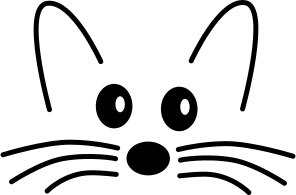
\includegraphics[width=1.4em]{squeak-logo}}}
\iftoshelse{
	\usepackage{marginnote}
		\renewcommand*{\marginfont}{\footnotesize}
	\newcommand{\vartriangleout}{\ifthenelse{\isodd{\thepage}}{\vartriangleright}{\vartriangleleft}}
	\newcommand{\dothisicon}{\fcolorbox{blue!65}{white}{\highlight{$\vartriangleout$}}}
	\newcommand{\dothis}[1]{%
		\noindent\par\noindent
		{\reversemarginpar
			\marginnote{\fcolorbox{blue!65}{white}{\highlight{$\vartriangleout$}}}}
		%\MarginLabel{do this}
		\noindent\emph{#1}
		\nopagebreak}
}{
	\newcommand{\dothisicon}{\raisebox{-.5ex}{
\includegraphics[height=1.2em]{pharo}}}
	\newcommand{\dothis}[1]{%
		\medskip
		\noindent\dothisicon
		\ifx#1\empty\else\quad\emph{#1}\fi
		\par\smallskip\nopagebreak}
}
%===> NEW VERSION <===
% NB: To use this in an individual chapter, you must set:
%\graphicspath{{figures/} {../figures/}}
% at the head of the chapter.  Don't forget the final /
%=============================================================
%:Reader hints (hint)
%
% Indicates a non-obvious consequence
\newcommand{\hint}[1]{\vspace{1ex}\noindent\fbox{\textsc{Hint}} \emph{#1}}
%=================================================================
% graphics for Morphic handles
\newcommand{\grabHandle}{\raisebox{-0.2ex}{
\includegraphics[width=1em]{blackHandle}}}
\newcommand{\moveHandle}{\raisebox{-0.2ex}{
\includegraphics[width=1em]{moveHandle}}}
\newcommand{\debugHandle}{\raisebox{-0.2ex}{
\includegraphics[width=1em]{debugHandle}}}
%=============================================================
%:Highlighting Important stuff (doublebox)
%
% From Seaside book ...
\newsavebox{\SavedText}
\newlength{\InnerBoxRule}\setlength{\InnerBoxRule}{.75\fboxrule}
\newlength{\OuterBoxRule}\setlength{\OuterBoxRule}{1.5\fboxrule}
\newlength{\BoxSeparation}\setlength{\BoxSeparation}{1.5\fboxrule}
\addtolength{\BoxSeparation}{.5pt}
\newlength{\SaveBoxSep}\setlength{\SaveBoxSep}{2\fboxsep}
%
\newenvironment{doublebox}{\begin{lrbox}{\SavedText}
    \begin{minipage}{.75\textwidth}}
    {\end{minipage}\end{lrbox}\begin{center}
    \setlength{\fboxsep}{\BoxSeparation}\setlength{\fboxrule}{\OuterBoxRule}
    \fbox{\setlength{\fboxsep}{\SaveBoxSep}\setlength{\fboxrule}{\InnerBoxRule}%
      \fbox{\usebox{\SavedText}}}
  \end{center}}
% Use this:
\newcommand{\important}[1]{\begin{doublebox}#1\end{doublebox}}
%=============================================================
%:Section depth
\setcounter{secnumdepth}{2}
%% for this to happen start the file with
%\ifx\wholebook\relax\else
%% $Author$
% $Date$
% $Revision$

% HISTORY:
% 2006-10-31 - Oscar code macros
% ...

%=============================================================
% NB: documentclass must be set in main document.
% Allows book to be generated in multiple formats.
%=============================================================
%:Packages
\usepackage[T1]{fontenc}  %%%%%% really important to get the code directly in the text!
\usepackage{lmodern}
%\usepackage[scaled=0.85]{bookmanx} % needs another scale factor if used with \renewcommand{\sfdefault}{cmbr}
\usepackage{palatino}
\usepackage[scaled=0.85]{helvet}
\usepackage[protrusion,expansion=false]{microtype}
\usepackage{graphicx}
\usepackage{theorem}
\usepackage[english]{babel}
% ON: pdfsync breaks the use of p{width} for tabular columns!
\ifdefined\usepdfsync\usepackage{pdfsync}\fi % Requires texlive 2007
%=============================================================
%:More packages
%Stef should check which ones are used!
%\usepackage{picinpar}
%\usepackage{layout}
%\usepackage{color}
%\usepackage{enum}
%\usepackage{a4wide}
% \usepackage{fancyhdr}
\usepackage{ifthen}
\usepackage{float}
\usepackage{longtable}
\usepackage{makeidx}
\usepackage[nottoc]{tocbibind}
\usepackage{multicol}
\usepackage{booktabs}	% book-style tables
\usepackage{topcapt}	% enables \topcaption
\usepackage{multirow}
\usepackage{tabularx}
%\usepackage[bottom]{footmisc}
\usepackage{xspace}
\usepackage{alltt}
\usepackage{amssymb,textcomp}
\usepackage[usenames,dvipsnames]{color}
%\usepackage{colortbl}
\usepackage[hang]{subfigure}\makeatletter\def\p@subfigure{\thefigure\,}\makeatother
\usepackage{rotating}
\usepackage{enumitem}	% apb: allows more control over tags in enumerations
\usepackage{verbatim}     % for comment environment
\usepackage{varioref}	% for page references that work
\labelformat{footnote}{\thechapter--#1} % to distinguish citations from jurabib
\usepackage{needspace}
\usepackage{isodateo} % enable \isodate
\usepackage[newparttoc,pagestyles]{titlesec}
\usepackage{titletoc}
\usepackage{wrapfig}

\usepackage[
	super,
	citefull=first,
	authorformat={allreversed,and},
	titleformat={commasep,italic}
]{jurabib} % citations as footnotes
\usepackage[
	colorlinks=true,
	linkcolor=black,
	urlcolor=black,
	citecolor=black
]{hyperref}   % should come last
%=============================================================
%:PDF version
\pdfminorversion=3 % Set PDF to 1.3 for Lulu
%=============================================================
%:URL style
\makeatletter
\def\url@leostyle{%
  \@ifundefined{selectfont}{\def\UrlFont{\sf}}{\def\UrlFont{\sffamily}}}
\makeatother
% Now actually use the newly defined style.
\urlstyle{leo}
%=============================================================
%:Booleans
\newboolean{lulu}
\setboolean{lulu}{false}
\newcommand{\ifluluelse}[2]{\ifthenelse{\boolean{lulu}}{#1}{#2}}
%=============================================================
%:Names
\newcommand{\SUnit}{SUnit\xspace}
\newcommand{\sunit}{SUnit\xspace}
\newcommand{\xUnit}{$x$Unit\xspace}
\newcommand{\JUnit}{JUnit\xspace}
\newcommand{\st}{Smalltalk\xspace}
\newcommand{\pharo}{Pharo\xspace} % Use this, not \Pharo
%\newcommand{\sqmap}{SqueakMap\xspace}
\newcommand{\squeak}{Squeak\xspace} % use this, not \Squeak or \sq
\newcommand{\sqsrc}{SqueakSource\xspace}
\newcommand{\sbe}{\url{http://SqueakByExample.org}\xspace}
\newcommand{\pharoweb}{\url{http://pharo-project.org}\xspace}
\newcommand{\pbe}{\url{http://PharoByExample.org}\xspace}
\newcommand{\sba}{\url{http://SquareBracketAssociates.org}\xspace}
\newcommand{\bam}{\lct{Bounc\-ing\-Atoms\-Morph}\xspace}
%=============================================================
%:Markup macros for proof-reading
\usepackage[normalem]{ulem} % for \sout
\usepackage{xcolor}
\newcommand{\ra}{$\rightarrow$}
\newcommand{\ugh}[1]{\textcolor{red}{\uwave{#1}}} % please rephrase
\newcommand{\ins}[1]{\textcolor{blue}{\uline{#1}}} % please insert
\newcommand{\del}[1]{\textcolor{red}{\sout{#1}}} % please delete
\newcommand{\chg}[2]{\textcolor{red}{\sout{#1}}{\ra}\textcolor{blue}{\uline{#2}}} % please change
%=============================================================
%:Editorial comment macros
%\newcommand{\nnbb}[2]{
%    % \fbox{\bfseries\sffamily\scriptsize#1}
%    \fcolorbox{gray}{yellow}{\bfseries\sffamily\scriptsize#1}
%    {\sf\small$\blacktriangleright$\textit{#2}$\blacktriangleleft$}
%   }
\newcommand{\yellowbox}[1]{\fcolorbox{gray}{yellow}{\bfseries\sffamily\scriptsize#1}}
\newcommand{\triangles}[1]{{\sf\small$\blacktriangleright$\textit{#1}$\blacktriangleleft$}}
\newcommand{\nnbb}[2]{\yellowbox{#1} \triangles{#2}}
\newcommand{\fix}{\yellowbox{FIX!}}
\newcommand{\here}{\yellowbox{CONTINUE HERE!}}
% editor macros
\newcommand{\apl}[1]{\nnbb{Alain}{#1}} % Alain
\newcommand{\ab}[1]{\nnbb{Andrew}{#1}} % Black
\newcommand{\sd}[1]{\nnbb{St\'{e}f}{#1}} % Ducasse
\newcommand{\gl}[1]{\nnbb{Guillaume}{#1}} % Ducasse
\newcommand{\cd}[1]{\nnbb{Christophe}{#1}} % Ducasse
\newcommand{\sig}[1]{\nnbb{Igor}{#1}} % Igor
\newcommand{\dc}[1]{\nnbb{DamienC}{#1}} % Ducasse
\newcommand{\md}[1]{\nnbb{Marcus}{#1}} % Denker
\newcommand{\on}[1]{\nnbb{Oscar}{#1}} % Nierstrasz
\newcommand{\damien}[1]{\nnbb{Damien}{#1}} % Pollet
\newcommand{\lr}[1]{\nnbb{Lukas}{#1}} % Renggli
\newcommand{\orla}[1]{\nnbb{Orla}{#1}} % Greevy
\newcommand{\alex}[1]{\nnbb{Alex}{#1}} % Bergel
\newcommand{\alx}[1]{\nnbb{Alex}{#1}} % Bergel
\newcommand{\dr}[1]{\nnbb{David}{#1}} % Roethlisberger
\newcommand{\ja}[1]{\nnbb{Jannik}{#1}} % Laval
\newcommand{\cb}[1]{\nnbb{Camillo}{#1}} % Bruni
\newcommand{\jr}[1]{\nnbb{Jorge}{#1}} % Ressia
\newcommand{\jb}[1]{\nnbb{JB}{#1}} % JB
\newcommand{\jp}[1]{\nnbb{Javier}{#1}} % Pimas
\newcommand{\fp}[1]{\nnbb{Fabrizio}{#1}} % Perin
\newcommand{\michael}[1]{\nnbb{Michael}{#1}} % Davies
\newcommand{\ew}[1]{\nnbb{Erwann}{#1}} % Wernli
\newcommand{\mb}[1]{\nnbb{Martial}{#1}} % Boniou
\newcommand{\hw}[1]{\nnbb{Hernan}{#1}} % Wilkinson
\newcommand{\ben}[1]{\nnbb{Benjamin}{#1}} % Benjamin Van Ryseghem
\newcommand{\hjo}[1]{\nnbb{HwaJong}{#1}} % HwaJong Oh aka daliot
\newcommand{\ml}[1]{\nnbb{Max}{#1}} % Max Leske
\newcommand{\mmp}[1]{\nnbb{Mariano}{#1}} % Mariano Martinez Peck
\newcommand{\luc}[1]{\nnbb{Luc}{#1}} % Luc Fabresse
\newcommand{\dkl}[1]{\nnbb{Daniel}{#1}} % Daniel Lyons
\newcommand{\vu}[1]{\nnbb{Veronica}{#1}} % Veronica Uquillas Gomez
\newcommand{\martin}[1]{\nnbb{Martin}{#1}} % Martin Dias
\newcommand{\vp}[1]{\nnbb{Vanessa}{#1}} % Vanessa Pena
\newcommand{\gp}[1]{\nnbb{Guille}{#1}} % Guillermo Polito

%=============================================================
%:Abbreviation macros
\newcommand{\ie}{\emph{i.e.},\xspace}
\newcommand{\eg}{\emph{e.g.},\xspace}
\newcommand{\etc}{etc.\xspace}
%=============================================================
%:Cross reference macros
\newcommand{\charef}[1]{Chapter~\ref{cha:#1}\xspace}
\newcommand{\secref}[1]{Section~\ref{sec:#1}\xspace}
\newcommand{\figref}[1]{Figure~\ref{fig:#1}\xspace}
\newcommand{\Figref}[1]{Figure~\ref{fig:#1}\xspace}
\newcommand{\appref}[1]{Appendix~\ref{app:#1}\xspace}
\newcommand{\tabref}[1]{Table~\ref{tab:#1}\xspace}
\newcommand{\faqref}[1]{FAQ~\ref{faq:#1}, p.~\pageref{faq:#1}\xspace}
% APB: I removed trailing \xspace commands from these macros because
% \xspace mostly doesn't work.  If you want a space after your
% references, type one!
% ON: xspace has always worked just fine for me!  Please leave them in.
%
\newcommand{\ruleref}[1]{\ref{rule:#1}\xspace}
%
\newcommand{\egref}[1]{example~\ref{eg:#1}\xspace}
\newcommand{\Egref}[1]{Example~\ref{eg:#1}\xspace}
%
\newcommand{\scrref}[1]{script~\ref{scr:#1}\xspace}
\newcommand{\Scrref}[1]{Script~\ref{scr:#1}\xspace}
\newcommand{\tscrref}[1]{the script~\ref{scr:#1}\xspace}
\newcommand{\Tscrref}[1]{The script~\ref{scr:#1}\xspace}
%
\newcommand{\mthref}[1]{method~\ref{mth:#1}\xspace}
\newcommand{\mthsref}[1]{methods~\ref{mth:#1}\xspace}
\newcommand{\Mthref}[1]{Method~\ref{mth:#1}\xspace}
\newcommand{\tmthref}[1]{the method~\ref{mth:#1}\xspace}
\newcommand{\Tmthref}[1]{The method~\ref{mth:#1}\xspace}
%
\newcommand{\clsref}[1]{class~\ref{cls:#1}\xspace}
\newcommand{\tclsref}[1]{the class~\ref{cls:#1}\xspace}
\newcommand{\Tclsref}[1]{The class~\ref{cls:#1}\xspace}

\newcommand{\chalabel}[1]{\label{cha:#1}}
\newcommand{\seclabel}[1]{\label{sec:#1}}
\newcommand{\figlabel}[1]{\label{fig:#1}}
\newcommand{\tablabel}[1]{\label{tab:#1}}
\newcommand{\rulelabel}[1]{\label{rule:#1}}
\newcommand{\eglabel}[1]{\label{eg:#1}}
\newcommand{\scrlabel}[1]{\label{scr:#1}}
\newcommand{\mthlabel}[1]{\label{mth:#1}}
\newcommand{\clslabel}[1]{\label{cls:#1}}
\newcommand{\faqlabel}[1]{\label{faq:#1}}
%=============================================================
%:Menu item macro
% for menu items, so we can change our minds on how to print them! (apb)
\definecolor{lightgray}{gray}{0.89}
\newcommand{\menu}[1]{{%
	\setlength{\fboxsep}{0pt}%
	\colorbox{lightgray}{{{\upshape\sffamily\strut \,#1\,}}}}}
\newcommand{\link}[1]{{%
	\fontfamily{lmr}\selectfont
 	\upshape{\sffamily \underline{#1}}}}
% For submenu items:
\newcommand{\go}{\,$\triangleright$\,}
% \newcommand{\go}{\,$\blacktriangleright$\,}
% For keyboard shortcuts:
%\newcommand{\short}[1]{\mbox{$\langle${\sc CMD}$\rangle$-#1}\xspace}
\newcommand{\short}[1]{\mbox{{\sc cmd}\hspace{0.08em}--\hspace{0.09em}#1}\xspace}
% For buttons:
\newcommand{\button}[1]{{%
	\setlength{\fboxsep}{0pt}%
	\fbox{{\upshape\sffamily\strut \,#1\,}}}}
% NB: The button macro does not work within captions -- incompatible with xcolor package :-(
\newcommand{\toolsflap}{\textit{Tools} flap\xspace}
%=============================================================
%:Mouse clicks
\newcommand{\click}{click\xspace} % RED
\newcommand{\actclick}{action-click\xspace} % YELLOW
\newcommand{\metaclick}{meta-click\xspace} % BLUE
\newcommand{\Click}{Click\xspace} % RED
\newcommand{\Actclick}{Action-click\xspace} % YELLOW
\newcommand{\Metaclick}{Meta-click\xspace} % BLUE
%=============================================================
%:ToSh macros
\newboolean{tosh}
\setboolean{tosh}{false}
\newcommand{\iftoshelse}[2]{\ifthenelse{\boolean{tosh}}{#1}{#2}}
%=============================================================
%:ToSh colors
%\newcommand{\highlightcolor}{\color{blue!65}}
%\newcommand{\boxcolor}{\color{gray!25}}
\newcommand{\highlight}[1]{\textcolor{blue!65}{#1}}
%\newcommand{\codecolor}{\color{blue!65}}
%%\setlength{\fboxrule}{2pt}
%\newcommand{\asPict}[1]{%
%	{\Large\highlight{#1}}}
%=============================================================
%:Reader cues (do this)
%
% Indicate something the reader should try out.
% \newcommand{\dothisicon}{\raisebox{-.5ex}{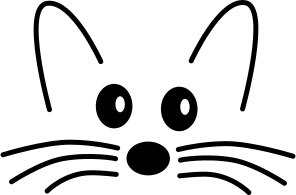
\includegraphics[width=1.4em]{squeak-logo}}}
\iftoshelse{
	\usepackage{marginnote}
		\renewcommand*{\marginfont}{\footnotesize}
	\newcommand{\vartriangleout}{\ifthenelse{\isodd{\thepage}}{\vartriangleright}{\vartriangleleft}}
	\newcommand{\dothisicon}{\fcolorbox{blue!65}{white}{\highlight{$\vartriangleout$}}}
	\newcommand{\dothis}[1]{%
		\noindent\par\noindent
		{\reversemarginpar
			\marginnote{\fcolorbox{blue!65}{white}{\highlight{$\vartriangleout$}}}}
		%\MarginLabel{do this}
		\noindent\emph{#1}
		\nopagebreak}
}{
	\newcommand{\dothisicon}{\raisebox{-.5ex}{
\includegraphics[height=1.2em]{pharo}}}
	\newcommand{\dothis}[1]{%
		\medskip
		\noindent\dothisicon
		\ifx#1\empty\else\quad\emph{#1}\fi
		\par\smallskip\nopagebreak}
}
%===> NEW VERSION <===
% NB: To use this in an individual chapter, you must set:
%\graphicspath{{figures/} {../figures/}}
% at the head of the chapter.  Don't forget the final /
%=============================================================
%:Reader hints (hint)
%
% Indicates a non-obvious consequence
\newcommand{\hint}[1]{\vspace{1ex}\noindent\fbox{\textsc{Hint}} \emph{#1}}
%=================================================================
% graphics for Morphic handles
\newcommand{\grabHandle}{\raisebox{-0.2ex}{
\includegraphics[width=1em]{blackHandle}}}
\newcommand{\moveHandle}{\raisebox{-0.2ex}{
\includegraphics[width=1em]{moveHandle}}}
\newcommand{\debugHandle}{\raisebox{-0.2ex}{
\includegraphics[width=1em]{debugHandle}}}
%=============================================================
%:Highlighting Important stuff (doublebox)
%
% From Seaside book ...
\newsavebox{\SavedText}
\newlength{\InnerBoxRule}\setlength{\InnerBoxRule}{.75\fboxrule}
\newlength{\OuterBoxRule}\setlength{\OuterBoxRule}{1.5\fboxrule}
\newlength{\BoxSeparation}\setlength{\BoxSeparation}{1.5\fboxrule}
\addtolength{\BoxSeparation}{.5pt}
\newlength{\SaveBoxSep}\setlength{\SaveBoxSep}{2\fboxsep}
%
\newenvironment{doublebox}{\begin{lrbox}{\SavedText}
    \begin{minipage}{.75\textwidth}}
    {\end{minipage}\end{lrbox}\begin{center}
    \setlength{\fboxsep}{\BoxSeparation}\setlength{\fboxrule}{\OuterBoxRule}
    \fbox{\setlength{\fboxsep}{\SaveBoxSep}\setlength{\fboxrule}{\InnerBoxRule}%
      \fbox{\usebox{\SavedText}}}
  \end{center}}
% Use this:
\newcommand{\important}[1]{\begin{doublebox}#1\end{doublebox}}
%=============================================================
%:Section depth
\setcounter{secnumdepth}{2}
%% for this to happen start the file with
%\ifx\wholebook\relax\else
%% $Author$
% $Date$
% $Revision$

% HISTORY:
% 2006-10-31 - Oscar code macros
% ...

%=============================================================
% NB: documentclass must be set in main document.
% Allows book to be generated in multiple formats.
%=============================================================
%:Packages
\usepackage[T1]{fontenc}  %%%%%% really important to get the code directly in the text!
\usepackage{lmodern}
%\usepackage[scaled=0.85]{bookmanx} % needs another scale factor if used with \renewcommand{\sfdefault}{cmbr}
\usepackage{palatino}
\usepackage[scaled=0.85]{helvet}
\usepackage[protrusion,expansion=false]{microtype}
\usepackage{graphicx}
\usepackage{theorem}
\usepackage[english]{babel}
% ON: pdfsync breaks the use of p{width} for tabular columns!
\ifdefined\usepdfsync\usepackage{pdfsync}\fi % Requires texlive 2007
%=============================================================
%:More packages
%Stef should check which ones are used!
%\usepackage{picinpar}
%\usepackage{layout}
%\usepackage{color}
%\usepackage{enum}
%\usepackage{a4wide}
% \usepackage{fancyhdr}
\usepackage{ifthen}
\usepackage{float}
\usepackage{longtable}
\usepackage{makeidx}
\usepackage[nottoc]{tocbibind}
\usepackage{multicol}
\usepackage{booktabs}	% book-style tables
\usepackage{topcapt}	% enables \topcaption
\usepackage{multirow}
\usepackage{tabularx}
%\usepackage[bottom]{footmisc}
\usepackage{xspace}
\usepackage{alltt}
\usepackage{amssymb,textcomp}
\usepackage[usenames,dvipsnames]{color}
%\usepackage{colortbl}
\usepackage[hang]{subfigure}\makeatletter\def\p@subfigure{\thefigure\,}\makeatother
\usepackage{rotating}
\usepackage{enumitem}	% apb: allows more control over tags in enumerations
\usepackage{verbatim}     % for comment environment
\usepackage{varioref}	% for page references that work
\labelformat{footnote}{\thechapter--#1} % to distinguish citations from jurabib
\usepackage{needspace}
\usepackage{isodateo} % enable \isodate
\usepackage[newparttoc,pagestyles]{titlesec}
\usepackage{titletoc}
\usepackage{wrapfig}

\usepackage[
	super,
	citefull=first,
	authorformat={allreversed,and},
	titleformat={commasep,italic}
]{jurabib} % citations as footnotes
\usepackage[
	colorlinks=true,
	linkcolor=black,
	urlcolor=black,
	citecolor=black
]{hyperref}   % should come last
%=============================================================
%:PDF version
\pdfminorversion=3 % Set PDF to 1.3 for Lulu
%=============================================================
%:URL style
\makeatletter
\def\url@leostyle{%
  \@ifundefined{selectfont}{\def\UrlFont{\sf}}{\def\UrlFont{\sffamily}}}
\makeatother
% Now actually use the newly defined style.
\urlstyle{leo}
%=============================================================
%:Booleans
\newboolean{lulu}
\setboolean{lulu}{false}
\newcommand{\ifluluelse}[2]{\ifthenelse{\boolean{lulu}}{#1}{#2}}
%=============================================================
%:Names
\newcommand{\SUnit}{SUnit\xspace}
\newcommand{\sunit}{SUnit\xspace}
\newcommand{\xUnit}{$x$Unit\xspace}
\newcommand{\JUnit}{JUnit\xspace}
\newcommand{\st}{Smalltalk\xspace}
\newcommand{\pharo}{Pharo\xspace} % Use this, not \Pharo
%\newcommand{\sqmap}{SqueakMap\xspace}
\newcommand{\squeak}{Squeak\xspace} % use this, not \Squeak or \sq
\newcommand{\sqsrc}{SqueakSource\xspace}
\newcommand{\sbe}{\url{http://SqueakByExample.org}\xspace}
\newcommand{\pharoweb}{\url{http://pharo-project.org}\xspace}
\newcommand{\pbe}{\url{http://PharoByExample.org}\xspace}
\newcommand{\sba}{\url{http://SquareBracketAssociates.org}\xspace}
\newcommand{\bam}{\lct{Bounc\-ing\-Atoms\-Morph}\xspace}
%=============================================================
%:Markup macros for proof-reading
\usepackage[normalem]{ulem} % for \sout
\usepackage{xcolor}
\newcommand{\ra}{$\rightarrow$}
\newcommand{\ugh}[1]{\textcolor{red}{\uwave{#1}}} % please rephrase
\newcommand{\ins}[1]{\textcolor{blue}{\uline{#1}}} % please insert
\newcommand{\del}[1]{\textcolor{red}{\sout{#1}}} % please delete
\newcommand{\chg}[2]{\textcolor{red}{\sout{#1}}{\ra}\textcolor{blue}{\uline{#2}}} % please change
%=============================================================
%:Editorial comment macros
%\newcommand{\nnbb}[2]{
%    % \fbox{\bfseries\sffamily\scriptsize#1}
%    \fcolorbox{gray}{yellow}{\bfseries\sffamily\scriptsize#1}
%    {\sf\small$\blacktriangleright$\textit{#2}$\blacktriangleleft$}
%   }
\newcommand{\yellowbox}[1]{\fcolorbox{gray}{yellow}{\bfseries\sffamily\scriptsize#1}}
\newcommand{\triangles}[1]{{\sf\small$\blacktriangleright$\textit{#1}$\blacktriangleleft$}}
\newcommand{\nnbb}[2]{\yellowbox{#1} \triangles{#2}}
\newcommand{\fix}{\yellowbox{FIX!}}
\newcommand{\here}{\yellowbox{CONTINUE HERE!}}
% editor macros
\newcommand{\apl}[1]{\nnbb{Alain}{#1}} % Alain
\newcommand{\ab}[1]{\nnbb{Andrew}{#1}} % Black
\newcommand{\sd}[1]{\nnbb{St\'{e}f}{#1}} % Ducasse
\newcommand{\gl}[1]{\nnbb{Guillaume}{#1}} % Ducasse
\newcommand{\cd}[1]{\nnbb{Christophe}{#1}} % Ducasse
\newcommand{\sig}[1]{\nnbb{Igor}{#1}} % Igor
\newcommand{\dc}[1]{\nnbb{DamienC}{#1}} % Ducasse
\newcommand{\md}[1]{\nnbb{Marcus}{#1}} % Denker
\newcommand{\on}[1]{\nnbb{Oscar}{#1}} % Nierstrasz
\newcommand{\damien}[1]{\nnbb{Damien}{#1}} % Pollet
\newcommand{\lr}[1]{\nnbb{Lukas}{#1}} % Renggli
\newcommand{\orla}[1]{\nnbb{Orla}{#1}} % Greevy
\newcommand{\alex}[1]{\nnbb{Alex}{#1}} % Bergel
\newcommand{\alx}[1]{\nnbb{Alex}{#1}} % Bergel
\newcommand{\dr}[1]{\nnbb{David}{#1}} % Roethlisberger
\newcommand{\ja}[1]{\nnbb{Jannik}{#1}} % Laval
\newcommand{\cb}[1]{\nnbb{Camillo}{#1}} % Bruni
\newcommand{\jr}[1]{\nnbb{Jorge}{#1}} % Ressia
\newcommand{\jb}[1]{\nnbb{JB}{#1}} % JB
\newcommand{\jp}[1]{\nnbb{Javier}{#1}} % Pimas
\newcommand{\fp}[1]{\nnbb{Fabrizio}{#1}} % Perin
\newcommand{\michael}[1]{\nnbb{Michael}{#1}} % Davies
\newcommand{\ew}[1]{\nnbb{Erwann}{#1}} % Wernli
\newcommand{\mb}[1]{\nnbb{Martial}{#1}} % Boniou
\newcommand{\hw}[1]{\nnbb{Hernan}{#1}} % Wilkinson
\newcommand{\ben}[1]{\nnbb{Benjamin}{#1}} % Benjamin Van Ryseghem
\newcommand{\hjo}[1]{\nnbb{HwaJong}{#1}} % HwaJong Oh aka daliot
\newcommand{\ml}[1]{\nnbb{Max}{#1}} % Max Leske
\newcommand{\mmp}[1]{\nnbb{Mariano}{#1}} % Mariano Martinez Peck
\newcommand{\luc}[1]{\nnbb{Luc}{#1}} % Luc Fabresse
\newcommand{\dkl}[1]{\nnbb{Daniel}{#1}} % Daniel Lyons
\newcommand{\vu}[1]{\nnbb{Veronica}{#1}} % Veronica Uquillas Gomez
\newcommand{\martin}[1]{\nnbb{Martin}{#1}} % Martin Dias
\newcommand{\vp}[1]{\nnbb{Vanessa}{#1}} % Vanessa Pena
\newcommand{\gp}[1]{\nnbb{Guille}{#1}} % Guillermo Polito

%=============================================================
%:Abbreviation macros
\newcommand{\ie}{\emph{i.e.},\xspace}
\newcommand{\eg}{\emph{e.g.},\xspace}
\newcommand{\etc}{etc.\xspace}
%=============================================================
%:Cross reference macros
\newcommand{\charef}[1]{Chapter~\ref{cha:#1}\xspace}
\newcommand{\secref}[1]{Section~\ref{sec:#1}\xspace}
\newcommand{\figref}[1]{Figure~\ref{fig:#1}\xspace}
\newcommand{\Figref}[1]{Figure~\ref{fig:#1}\xspace}
\newcommand{\appref}[1]{Appendix~\ref{app:#1}\xspace}
\newcommand{\tabref}[1]{Table~\ref{tab:#1}\xspace}
\newcommand{\faqref}[1]{FAQ~\ref{faq:#1}, p.~\pageref{faq:#1}\xspace}
% APB: I removed trailing \xspace commands from these macros because
% \xspace mostly doesn't work.  If you want a space after your
% references, type one!
% ON: xspace has always worked just fine for me!  Please leave them in.
%
\newcommand{\ruleref}[1]{\ref{rule:#1}\xspace}
%
\newcommand{\egref}[1]{example~\ref{eg:#1}\xspace}
\newcommand{\Egref}[1]{Example~\ref{eg:#1}\xspace}
%
\newcommand{\scrref}[1]{script~\ref{scr:#1}\xspace}
\newcommand{\Scrref}[1]{Script~\ref{scr:#1}\xspace}
\newcommand{\tscrref}[1]{the script~\ref{scr:#1}\xspace}
\newcommand{\Tscrref}[1]{The script~\ref{scr:#1}\xspace}
%
\newcommand{\mthref}[1]{method~\ref{mth:#1}\xspace}
\newcommand{\mthsref}[1]{methods~\ref{mth:#1}\xspace}
\newcommand{\Mthref}[1]{Method~\ref{mth:#1}\xspace}
\newcommand{\tmthref}[1]{the method~\ref{mth:#1}\xspace}
\newcommand{\Tmthref}[1]{The method~\ref{mth:#1}\xspace}
%
\newcommand{\clsref}[1]{class~\ref{cls:#1}\xspace}
\newcommand{\tclsref}[1]{the class~\ref{cls:#1}\xspace}
\newcommand{\Tclsref}[1]{The class~\ref{cls:#1}\xspace}

\newcommand{\chalabel}[1]{\label{cha:#1}}
\newcommand{\seclabel}[1]{\label{sec:#1}}
\newcommand{\figlabel}[1]{\label{fig:#1}}
\newcommand{\tablabel}[1]{\label{tab:#1}}
\newcommand{\rulelabel}[1]{\label{rule:#1}}
\newcommand{\eglabel}[1]{\label{eg:#1}}
\newcommand{\scrlabel}[1]{\label{scr:#1}}
\newcommand{\mthlabel}[1]{\label{mth:#1}}
\newcommand{\clslabel}[1]{\label{cls:#1}}
\newcommand{\faqlabel}[1]{\label{faq:#1}}
%=============================================================
%:Menu item macro
% for menu items, so we can change our minds on how to print them! (apb)
\definecolor{lightgray}{gray}{0.89}
\newcommand{\menu}[1]{{%
	\setlength{\fboxsep}{0pt}%
	\colorbox{lightgray}{{{\upshape\sffamily\strut \,#1\,}}}}}
\newcommand{\link}[1]{{%
	\fontfamily{lmr}\selectfont
 	\upshape{\sffamily \underline{#1}}}}
% For submenu items:
\newcommand{\go}{\,$\triangleright$\,}
% \newcommand{\go}{\,$\blacktriangleright$\,}
% For keyboard shortcuts:
%\newcommand{\short}[1]{\mbox{$\langle${\sc CMD}$\rangle$-#1}\xspace}
\newcommand{\short}[1]{\mbox{{\sc cmd}\hspace{0.08em}--\hspace{0.09em}#1}\xspace}
% For buttons:
\newcommand{\button}[1]{{%
	\setlength{\fboxsep}{0pt}%
	\fbox{{\upshape\sffamily\strut \,#1\,}}}}
% NB: The button macro does not work within captions -- incompatible with xcolor package :-(
\newcommand{\toolsflap}{\textit{Tools} flap\xspace}
%=============================================================
%:Mouse clicks
\newcommand{\click}{click\xspace} % RED
\newcommand{\actclick}{action-click\xspace} % YELLOW
\newcommand{\metaclick}{meta-click\xspace} % BLUE
\newcommand{\Click}{Click\xspace} % RED
\newcommand{\Actclick}{Action-click\xspace} % YELLOW
\newcommand{\Metaclick}{Meta-click\xspace} % BLUE
%=============================================================
%:ToSh macros
\newboolean{tosh}
\setboolean{tosh}{false}
\newcommand{\iftoshelse}[2]{\ifthenelse{\boolean{tosh}}{#1}{#2}}
%=============================================================
%:ToSh colors
%\newcommand{\highlightcolor}{\color{blue!65}}
%\newcommand{\boxcolor}{\color{gray!25}}
\newcommand{\highlight}[1]{\textcolor{blue!65}{#1}}
%\newcommand{\codecolor}{\color{blue!65}}
%%\setlength{\fboxrule}{2pt}
%\newcommand{\asPict}[1]{%
%	{\Large\highlight{#1}}}
%=============================================================
%:Reader cues (do this)
%
% Indicate something the reader should try out.
% \newcommand{\dothisicon}{\raisebox{-.5ex}{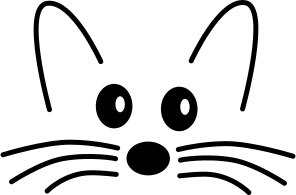
\includegraphics[width=1.4em]{squeak-logo}}}
\iftoshelse{
	\usepackage{marginnote}
		\renewcommand*{\marginfont}{\footnotesize}
	\newcommand{\vartriangleout}{\ifthenelse{\isodd{\thepage}}{\vartriangleright}{\vartriangleleft}}
	\newcommand{\dothisicon}{\fcolorbox{blue!65}{white}{\highlight{$\vartriangleout$}}}
	\newcommand{\dothis}[1]{%
		\noindent\par\noindent
		{\reversemarginpar
			\marginnote{\fcolorbox{blue!65}{white}{\highlight{$\vartriangleout$}}}}
		%\MarginLabel{do this}
		\noindent\emph{#1}
		\nopagebreak}
}{
	\newcommand{\dothisicon}{\raisebox{-.5ex}{
\includegraphics[height=1.2em]{pharo}}}
	\newcommand{\dothis}[1]{%
		\medskip
		\noindent\dothisicon
		\ifx#1\empty\else\quad\emph{#1}\fi
		\par\smallskip\nopagebreak}
}
%===> NEW VERSION <===
% NB: To use this in an individual chapter, you must set:
%\graphicspath{{figures/} {../figures/}}
% at the head of the chapter.  Don't forget the final /
%=============================================================
%:Reader hints (hint)
%
% Indicates a non-obvious consequence
\newcommand{\hint}[1]{\vspace{1ex}\noindent\fbox{\textsc{Hint}} \emph{#1}}
%=================================================================
% graphics for Morphic handles
\newcommand{\grabHandle}{\raisebox{-0.2ex}{
\includegraphics[width=1em]{blackHandle}}}
\newcommand{\moveHandle}{\raisebox{-0.2ex}{
\includegraphics[width=1em]{moveHandle}}}
\newcommand{\debugHandle}{\raisebox{-0.2ex}{
\includegraphics[width=1em]{debugHandle}}}
%=============================================================
%:Highlighting Important stuff (doublebox)
%
% From Seaside book ...
\newsavebox{\SavedText}
\newlength{\InnerBoxRule}\setlength{\InnerBoxRule}{.75\fboxrule}
\newlength{\OuterBoxRule}\setlength{\OuterBoxRule}{1.5\fboxrule}
\newlength{\BoxSeparation}\setlength{\BoxSeparation}{1.5\fboxrule}
\addtolength{\BoxSeparation}{.5pt}
\newlength{\SaveBoxSep}\setlength{\SaveBoxSep}{2\fboxsep}
%
\newenvironment{doublebox}{\begin{lrbox}{\SavedText}
    \begin{minipage}{.75\textwidth}}
    {\end{minipage}\end{lrbox}\begin{center}
    \setlength{\fboxsep}{\BoxSeparation}\setlength{\fboxrule}{\OuterBoxRule}
    \fbox{\setlength{\fboxsep}{\SaveBoxSep}\setlength{\fboxrule}{\InnerBoxRule}%
      \fbox{\usebox{\SavedText}}}
  \end{center}}
% Use this:
\newcommand{\important}[1]{\begin{doublebox}#1\end{doublebox}}
%=============================================================
%:Section depth
\setcounter{secnumdepth}{2}
%% for this to happen start the file with
%\ifx\wholebook\relax\else
%\input{../common.tex}
%\begin{document}
%\fi
% and terminate by
% \ifx\wholebook\relax\else\end{document}\fi

\DeclareGraphicsExtensions{.pdf, .jpg, .png}
%=============================================================
%:PDF setup
\hypersetup{
%   a4paper,
%   pdfstartview=FitV,
%   colorlinks,
%   linkcolor=darkblue,
%   citecolor=darkblue,
   pdftitle={Pharo by Example},
   pdfauthor={Andrew P. Black, St\'ephane Ducasse,	Oscar Nierstrasz,
Damien Pollet},
   pdfkeywords={Smalltalk, Squeak, Object-Oriented Programming, OOP},
   pdfsubject={Computer Science}
}
%=============================================================
%:Page layout and appearance
%
% \renewcommand{\headrulewidth}{0pt}
\renewcommand{\chaptermark}[1]{\markboth{#1}{}}
\renewcommand{\sectionmark}[1]{\markright{\thesection\ #1}}
\renewpagestyle{plain}[\small\itshape]{%
	\setheadrule{0pt}%
	\sethead[][][]{}{}{}%
	\setfoot[][][]{}{}{}}
\renewpagestyle{headings}[\small\itshape]{%
	\setheadrule{0pt}%
	\setmarks{chapter}{section}%
	\sethead[\thepage][][\chaptertitle]{\sectiontitle}{}{\thepage}%
	\setfoot[][][]{}{}{}}
%=============================================================
%:Title section setup and TOC numbering depth
\setcounter{secnumdepth}{1}
\setcounter{tocdepth}{1}
\titleformat{\part}[display]{\centering}{\huge\partname\ \thepart}{1em}{\Huge\textbf}[]
\titleformat{\chapter}[display]{}{\huge\chaptertitlename\ \thechapter}{1em}{\Huge\raggedright\textbf}[]
\titlecontents{part}[3pc]{%
		\pagebreak[2]\addvspace{1em plus.4em minus.2em}%
		\leavevmode\large\bfseries}
	{\contentslabel{3pc}}{\hspace*{-3pc}}
	{}[\nopagebreak]
\titlecontents{chapter}[3pc]{%
		\pagebreak[0]\addvspace{1em plus.2em minus.2em}%
		\leavevmode\bfseries}
	{\contentslabel{3pc}}{}
	{\hfill\contentspage}[\nopagebreak]
\dottedcontents{section}[3pc]{}{3pc}{1pc}
\dottedcontents{subsection}[3pc]{}{0pc}{1pc}
% \dottedcontents{subsection}[4.5em]{}{0pt}{1pc}
% Make \cleardoublepage insert really blank pages http://www.tex.ac.uk/cgi-bin/texfaq2html?label=reallyblank
\let\origdoublepage\cleardoublepage
\newcommand{\clearemptydoublepage}{%
  \clearpage
  {\pagestyle{empty}\origdoublepage}}
\let\cleardoublepage\clearemptydoublepage % see http://www.tex.ac.uk/cgi-bin/texfaq2html?label=patch
%=============================================================
%:FAQ macros (for FAQ chapter)
\newtheorem{faq}{FAQ}
\newcommand{\answer}{\paragraph{Answer}\ }
%=============================================================
%:Listings package configuration
% \newcommand{\caret}{\makebox{\raisebox{0.4ex}{\footnotesize{$\wedge$}}}}
\newcommand{\caret}{\^\,}
\newcommand{\escape}{{\sf \textbackslash}}
\definecolor{source}{gray}{0.95}
\usepackage{listings}
\lstdefinelanguage{Smalltalk}{
%  morekeywords={self,super,true,false,nil,thisContext}, % This is overkill
  morestring=[d]',
  morecomment=[s]{"}{"},
  alsoletter={\#:},
  escapechar={!},
  literate=
    {BANG}{!}1
    {CARET}{\^}1
    {UNDERSCORE}{\_}1
    {\\st}{Smalltalk}9 % convenience -- in case \st occurs in code
    % {'}{{\textquotesingle}}1 % replaced by upquote=true in \lstset
    %{_}{{$\leftarrow$}}1
    {>>>}{{\sep}}1
    %{^}{{$\uparrow$}}1
    {~}{{$\sim$}}1
    {-}{{\texttt{-}}}1 %{\textminus}}1 %{-}{\hspace{-0.13em}}{-}}1  % the goal is to make - the same width as +
    % {+}{\sf+}1 %{\raisebox{0.08ex}{+}}}1      % and to raise + off the baseline to match -
    {-->}{{\quad$\longrightarrow$\quad}}3
    {~->}{{\quad$\leadsto$\quad}}3
	, % Don't forget the comma at the end!
  tabsize=4
}[keywords,comments,strings]

\lstset{language=Smalltalk,
	basicstyle=\sffamily,
	keywordstyle=\color{black}\bfseries,
	% stringstyle=\ttfamily, % Ugly! do we really want this? -- on
	mathescape=true,
	showstringspaces=false,
	keepspaces=true,
	breaklines=true,
	breakautoindent=true,
	backgroundcolor=\color{source},
	lineskip={-1pt}, % Ugly hack
	upquote=true, % straight quote; requires textcomp package
	columns=fullflexible} % no fixed width fonts
% In-line code (literal)
% Normally use this for all in-line code:

\newcommand{\ct}{\lstinline[mathescape=false,backgroundcolor=\color{white},basicstyle={\sffamily\upshape}]}
\newcommand{\cts}[1]{{\sffamily{\upshape{#1}}\xspace}}
% apb 2007.8.28 added the \upshape declaration to avoid getting italicized code in \dothis{ } sections.
% In-line code (latex enabled)
% Use this only in special situations where \ct does not work
% (within section headings ...):
\newcommand{\lct}[1]{{\textsf{\textup{#1}}}}
% Use these for system categories and protocols:
\newcommand{\scat}[1]{\emph{\textsf{#1}}\xspace}
\newcommand{\pkg}[1]{\emph{\textsf{#1}}\xspace}
\newcommand{\prot}[1]{\emph{\textsf{#1}}\xspace}
% Code environments
% NB: the arg is for tests
% Only code and example environments may be tests
\lstnewenvironment{code}[1]{%
	\lstset{%
		% frame=lines,
		frame=single,
		framerule=0pt,
		mathescape=false
	}
}{}
\def\ignoredollar#1{}
%=============================================================
%:Code environments (method, script ...)
% NB: the third arg is for tests
% Only code and example environments may be tests
\lstnewenvironment{example}[3][defaultlabel]{%
	\renewcommand{\lstlistingname}{Example}%
	\lstset{
		% frame=lines,
		frame=single,
		framerule=0pt,
		mathescape=false,
		caption={\emph{#2}},
		label={eg:#1}
	}
}{}
\lstnewenvironment{script}[2][defaultlabel]{%
\renewcommand{\lstlistingname}{Script}%
	\lstset{
		% frame=lines,
		frame=single,
		framerule=0pt,
		mathescape=false,
		name={Script},
		caption={\emph{#2}},
		label={scr:#1}
	}
}{}
\lstnewenvironment{method}[2][defaultlabel]{%
	\renewcommand{\lstlistingname}{Method}%
	\lstset{
		% frame=lines,
		frame=single,
		framerule=0pt,
		mathescape=false,
		name={Method},
		caption={\emph{#2}},
		label={mth:#1}
	}
}{}
\lstnewenvironment{methods}[2][defaultlabel]{% just for multiple methods at once
	\renewcommand{\lstlistingname}{Methods}%
	\lstset{
		% frame=lines,
		frame=single,
		framerule=0pt,
		mathescape=false,
		name={Method},
		caption={\emph{#2}},
		label={mth:#1}
	}
}{}
\lstnewenvironment{numMethod}[2][defaultlabel]{%
	\renewcommand{\lstlistingname}{Method}%
	\lstset{
		numbers=left,
		numberstyle={\tiny\sffamily},
		% frame=lines,
		frame=single,
		framerule=0pt,
		mathescape=false,
		name={Method},
		caption={\emph{#2}},
		label={mth:#1}
	}
}{}
\lstnewenvironment{classdef}[2][defaultlabel]{%
	\renewcommand{\lstlistingname}{Class}%
	\lstset{
		% frame=lines,
		frame=single,
		framerule=0pt,
		mathescape=false,
		name={Class},
		caption={\emph{#2}},
		label={cls:#1}
	}
}{}
%=============================================================
%:Reserving space
% Usually need one more line than the actual lines of code
\newcommand{\needlines}[1]{\Needspace{#1\baselineskip}}
%=============================================================
%:Indexing macros
% Macros ending with "ind" generate text as well as an index entry
% Macros ending with "index" *only* generate an index entry
\newcommand{\ind}[1]{\index{#1}#1\xspace} % plain text
\newcommand{\subind}[2]{\index{#1!#2}#2\xspace} % show #2, subindex under #1
\newcommand{\emphind}[1]{\index{#1}\emph{#1}\xspace} % emph #1
\newcommand{\emphsubind}[2]{\index{#1!#2}\emph{#2}\xspace} % show emph #2, subindex inder #1
\newcommand{\scatind}[1]{\index{#1@\textsf{#1} (category)}\scat{#1}} % category
\newcommand{\pkgind}[1]{\index{#1@\textsf{#1} (package)}\pkg{#1}} % package
\newcommand{\protind}[1]{\index{#1@\textsf{#1} (protocol)}\prot{#1}} % protocol
\newcommand{\clsind}[1]{\index{#1@\textsf{#1} (class)}\ct{#1}\xspace}
% \newcommand{\clsind}[1]{\index{#1!\#@(class)}\ct{#1}\xspace} % class
\newcommand{\clsindplural}[1]{\index{#1!\#@(class)}\ct{#1}s\xspace} % class
\newcommand{\cvind}[1]{\index{#1@\textsf{#1} (class variable)}\ct{#1}\xspace} % class var
\newcommand{\glbind}[1]{\index{#1@\textsf{#1} (global)}\ct{#1}\xspace} % global
\newcommand{\patind}[1]{\index{#1@#1 (pattern)}\ct{#1}\xspace} % pattern
\newcommand{\pvind}[1]{\index{#1@\textsf{#1} (pseudo variable)}\ct{#1}\xspace} % pseudo var
\newcommand{\clsmthind}[2]{\index{#1!#2@\ct{#2}}\ct{#1>>>#2}\xspace} % class + method name
\newcommand{\mthind}[2]{\index{#1!#2@\ct{#2}}\ct{#2}\xspace} % show method name only
\newcommand{\lmthind}[2]{\index{#1!#2@\ct{#2}}\lct{#2}\xspace} % show method name only
\newcommand{\cmind}[2]{\index{#1!#2@\ct{#2}}\ct{#1>>>#2}\xspace} % show class>>method
\newcommand{\lcmind}[2]{\index{#1!#2@\ct{#2}}\lct{#1>>>#2}\xspace} % show class>>method
\newcommand{\toolsflapind}{\index{Tools flap}\toolsflap} % index tools flap
% The following only generate an index entry:
% \newcommand{\clsindex}[1]{\index{#1@\textsf{#1} (class)}}
\newcommand{\clsindex}[1]{\index{#1!\#@(class)}} % class
\newcommand{\mthindex}[2]{\index{#1!#2@\ct{#2}}} % method
\newcommand{\cmindex}[2]{\index{#1!#2@\ct{#2}}} % class>>method
\newcommand{\cvindex}[1]{\index{#1@\textsf{#1} (class variable)}} % class var
\newcommand{\glbindex}[1]{\index{#1@\textsf{#1} (global)}}% global
\newcommand{\pvindex}[1]{\index{#1@\textsf{#1} (pseudo variable)}}% pseudo var
\newcommand{\seeindex}[2]{\index{#1|see{#2}}} % #1, see #2
\newcommand{\scatindex}[1]{\index{#1@\textsf{#1} (category)}} % category
\newcommand{\pkgindex}[1]{\index{#1@\textsf{#1} (package)}} % package
\newcommand{\protindex}[1]{\index{#1@\textsf{#1} (protocol)}} % protocol
% How can we have the main entry page numbers in bold yet not break the hyperlink?
\newcommand{\boldidx}[1]{{\bf #1}} % breaks hyperlink
%\newcommand{\indmain}[1]{\index{#1|boldidx}#1\xspace} % plain text, main entry
%\newcommand{\emphsubindmain}[2]{\index{#1!#2|boldidx}\emph{#2}\xspace} % subindex, main entry
%\newcommand{\subindmain}[2]{\index{#1!#2|boldidx}#2\xspace} % subindex, main entry
%\newcommand{\clsindmain}[1]{\index{#1@\textsf{#1} (class)|boldidx}\ct{#1}\xspace}
%\newcommand{\clsindmain}[1]{\index{#1!\#@(class)|boldidx}\ct{#1}\xspace} % class main
%\newcommand{\indexmain}[1]{\index{#1|boldidx}} % main index entry only
\newcommand{\indmain}[1]{\index{#1}#1\xspace} % The main index entry for this item
\newcommand{\emphsubindmain}[2]{\index{#1!#2}\emph{#2}\xspace} % subindex, main entry
\newcommand{\subindmain}[2]{\index{#1!#2}#2\xspace} % subindex, main entry
%\newcommand{\clsindmain}[1]{\index{#1@\textsf{#1} (class)}\ct{#1}\xspace}
\newcommand{\clsindmain}[1]{\index{#1!\#@(class)}\ct{#1}\xspace} % class main
\newcommand{\clsindexmain}[1]{\index{#1!\#@(class)}} % class main index only
\newcommand{\indexmain}[1]{\index{#1}}
%=============================================================
%:Code macros
% some constants
\newcommand{\codesize}{\small}
\newcommand{\codefont}{\sffamily}
%\newcommand{\cat}[1]{\textit{In category #1}}%%To remove later
\newlength{\scriptindent}
\setlength{\scriptindent}{.3cm}
%% Method presentation constants
\newlength{\methodindent}
\newlength{\methodwordlength}
\newlength{\aftermethod}
\setlength{\methodindent}{0.2cm}
\settowidth{\methodwordlength}{\ M\'ethode\ }
%=============================================================
%:Smalltalk macros
%\newcommand{\sep}{{$\gg$}}
\newcommand{\sep}{\mbox{>>}}
\newcommand{\self}{\lct{self}\xspace}
\newcommand{\super}{\lct{super}\xspace}
\newcommand{\nil}{\lct{nil}\xspace}
%=============================================================
% be less conservative about float placement
% these commands are from http://www.tex.ac.uk/cgi-bin/texfaq2html?label=floats
\renewcommand{\topfraction}{.9}
\renewcommand{\bottomfraction}{.9}
\renewcommand{\textfraction}{.1}
\renewcommand{\floatpagefraction}{.85}
\renewcommand{\dbltopfraction}{.66}
\renewcommand{\dblfloatpagefraction}{.85}
\setcounter{topnumber}{9}
\setcounter{bottomnumber}{9}
\setcounter{totalnumber}{20}
\setcounter{dbltopnumber}{9}
%=============================================================
% Give information from each chapter's author
\newcommand{\contact}[2]{\textbf{#1} \textsf{(#2)}}

\newcommand{\chapterauthor}[1]{\emph{with the participation of:\\#1}\\}
\newcommand{\chapterwritten}[1]{\emph{written by:\\#1}\\}

\newcommand{\authornoury}{\contact{Noury Bouraqadi}{Noury.Bouraqadi@mines-douai.fr}}
\newcommand{\authorluc}{\contact{Luc Fabresse}{Luc.Fabresse@mines-douai.fr}}
\newcommand{\authordamienc}{\contact{Damien Cassou}{damien.cassou@gmail.com}}
\newcommand{\authoroscar}{\contact{Oscar Nierstrasz}{oscar.nierstrasz@acm.org}}
\newcommand{\authorsteph}{\contact{St\'ephane Ducasse}{stephane.ducasse@inria.fr}}
\newcommand{\authoralex}{\contact{Alexandre Bergel}{alexandre@bergel.eu}}
\newcommand{\authorolivier}{\contact{Olivier Auverlot}{olivier.auverlot@inria.fr}}
\newcommand{\authornicolas}{\contact{Nicolas Cellier}{nicolas.cellier.aka.nice@gmail.com}}
\newcommand{\authormarcus}{\contact{Marcus Denker}{marcus.denker@inria.fr}}
\newcommand{\authoralain}{\contact{Alain Plantec}{alain.plantec@univ-brest.fr}}
\newcommand{\authordale}{\contact{Dale Henrichs}{dale.henrichs@gemstone.com}}
\newcommand{\authormariano}{\contact{Mariano Martinez Peck}{marianopeck@gmail.com}}
\newcommand{\authorsven}{\contact{Sven Van Caekenberghe}{sven@beta9.be}}
\newcommand{\authorlukas}{\contact{Lukas Renggli}{renggli@gmail.com}}
\newcommand{\authorjankurs}{\contact{Jan Kurs}{kurs@iam.unibe.ch}}
\newcommand{\authorguillaume}{\contact{Guillaume Larcheveque}{guillaume.larcheveque@gmail.com}}
\newcommand{\authorguillep}{\contact{Guillermo Polito}{guillermopolito@gmail.com}}
\newcommand{\authorclement}{\contact{Cl\'ement Bera}{bera.clement@gmail.com}}
\newcommand{\authormax}{\contact{Max Leske}{maxleske@gmail.com}}
\newcommand{\authorvanessa}{\contact{Vanessa Pe\~{n}a-Araya}{van.c.pena@gmail.com}}
\newcommand{\authorcamillo}{\contact{Camillo Bruni}{camillobruni@gmail.com}}

%=============================================================
% apb doesn't like paragraphs to run in to each other without a break
\parskip 1ex
%=============================================================
%:Stuff to check, merge or deprecate
%\setlength{\marginparsep}{2mm}
%\renewcommand{\baselinestretch}{1.1}
%=============================================================
\usepackage{tikz}

%\begin{document}
%\fi
% and terminate by
% \ifx\wholebook\relax\else\end{document}\fi

\DeclareGraphicsExtensions{.pdf, .jpg, .png}
%=============================================================
%:PDF setup
\hypersetup{
%   a4paper,
%   pdfstartview=FitV,
%   colorlinks,
%   linkcolor=darkblue,
%   citecolor=darkblue,
   pdftitle={Pharo by Example},
   pdfauthor={Andrew P. Black, St\'ephane Ducasse,	Oscar Nierstrasz,
Damien Pollet},
   pdfkeywords={Smalltalk, Squeak, Object-Oriented Programming, OOP},
   pdfsubject={Computer Science}
}
%=============================================================
%:Page layout and appearance
%
% \renewcommand{\headrulewidth}{0pt}
\renewcommand{\chaptermark}[1]{\markboth{#1}{}}
\renewcommand{\sectionmark}[1]{\markright{\thesection\ #1}}
\renewpagestyle{plain}[\small\itshape]{%
	\setheadrule{0pt}%
	\sethead[][][]{}{}{}%
	\setfoot[][][]{}{}{}}
\renewpagestyle{headings}[\small\itshape]{%
	\setheadrule{0pt}%
	\setmarks{chapter}{section}%
	\sethead[\thepage][][\chaptertitle]{\sectiontitle}{}{\thepage}%
	\setfoot[][][]{}{}{}}
%=============================================================
%:Title section setup and TOC numbering depth
\setcounter{secnumdepth}{1}
\setcounter{tocdepth}{1}
\titleformat{\part}[display]{\centering}{\huge\partname\ \thepart}{1em}{\Huge\textbf}[]
\titleformat{\chapter}[display]{}{\huge\chaptertitlename\ \thechapter}{1em}{\Huge\raggedright\textbf}[]
\titlecontents{part}[3pc]{%
		\pagebreak[2]\addvspace{1em plus.4em minus.2em}%
		\leavevmode\large\bfseries}
	{\contentslabel{3pc}}{\hspace*{-3pc}}
	{}[\nopagebreak]
\titlecontents{chapter}[3pc]{%
		\pagebreak[0]\addvspace{1em plus.2em minus.2em}%
		\leavevmode\bfseries}
	{\contentslabel{3pc}}{}
	{\hfill\contentspage}[\nopagebreak]
\dottedcontents{section}[3pc]{}{3pc}{1pc}
\dottedcontents{subsection}[3pc]{}{0pc}{1pc}
% \dottedcontents{subsection}[4.5em]{}{0pt}{1pc}
% Make \cleardoublepage insert really blank pages http://www.tex.ac.uk/cgi-bin/texfaq2html?label=reallyblank
\let\origdoublepage\cleardoublepage
\newcommand{\clearemptydoublepage}{%
  \clearpage
  {\pagestyle{empty}\origdoublepage}}
\let\cleardoublepage\clearemptydoublepage % see http://www.tex.ac.uk/cgi-bin/texfaq2html?label=patch
%=============================================================
%:FAQ macros (for FAQ chapter)
\newtheorem{faq}{FAQ}
\newcommand{\answer}{\paragraph{Answer}\ }
%=============================================================
%:Listings package configuration
% \newcommand{\caret}{\makebox{\raisebox{0.4ex}{\footnotesize{$\wedge$}}}}
\newcommand{\caret}{\^\,}
\newcommand{\escape}{{\sf \textbackslash}}
\definecolor{source}{gray}{0.95}
\usepackage{listings}
\lstdefinelanguage{Smalltalk}{
%  morekeywords={self,super,true,false,nil,thisContext}, % This is overkill
  morestring=[d]',
  morecomment=[s]{"}{"},
  alsoletter={\#:},
  escapechar={!},
  literate=
    {BANG}{!}1
    {CARET}{\^}1
    {UNDERSCORE}{\_}1
    {\\st}{Smalltalk}9 % convenience -- in case \st occurs in code
    % {'}{{\textquotesingle}}1 % replaced by upquote=true in \lstset
    %{_}{{$\leftarrow$}}1
    {>>>}{{\sep}}1
    %{^}{{$\uparrow$}}1
    {~}{{$\sim$}}1
    {-}{{\texttt{-}}}1 %{\textminus}}1 %{-}{\hspace{-0.13em}}{-}}1  % the goal is to make - the same width as +
    % {+}{\sf+}1 %{\raisebox{0.08ex}{+}}}1      % and to raise + off the baseline to match -
    {-->}{{\quad$\longrightarrow$\quad}}3
    {~->}{{\quad$\leadsto$\quad}}3
	, % Don't forget the comma at the end!
  tabsize=4
}[keywords,comments,strings]

\lstset{language=Smalltalk,
	basicstyle=\sffamily,
	keywordstyle=\color{black}\bfseries,
	% stringstyle=\ttfamily, % Ugly! do we really want this? -- on
	mathescape=true,
	showstringspaces=false,
	keepspaces=true,
	breaklines=true,
	breakautoindent=true,
	backgroundcolor=\color{source},
	lineskip={-1pt}, % Ugly hack
	upquote=true, % straight quote; requires textcomp package
	columns=fullflexible} % no fixed width fonts
% In-line code (literal)
% Normally use this for all in-line code:

\newcommand{\ct}{\lstinline[mathescape=false,backgroundcolor=\color{white},basicstyle={\sffamily\upshape}]}
\newcommand{\cts}[1]{{\sffamily{\upshape{#1}}\xspace}}
% apb 2007.8.28 added the \upshape declaration to avoid getting italicized code in \dothis{ } sections.
% In-line code (latex enabled)
% Use this only in special situations where \ct does not work
% (within section headings ...):
\newcommand{\lct}[1]{{\textsf{\textup{#1}}}}
% Use these for system categories and protocols:
\newcommand{\scat}[1]{\emph{\textsf{#1}}\xspace}
\newcommand{\pkg}[1]{\emph{\textsf{#1}}\xspace}
\newcommand{\prot}[1]{\emph{\textsf{#1}}\xspace}
% Code environments
% NB: the arg is for tests
% Only code and example environments may be tests
\lstnewenvironment{code}[1]{%
	\lstset{%
		% frame=lines,
		frame=single,
		framerule=0pt,
		mathescape=false
	}
}{}
\def\ignoredollar#1{}
%=============================================================
%:Code environments (method, script ...)
% NB: the third arg is for tests
% Only code and example environments may be tests
\lstnewenvironment{example}[3][defaultlabel]{%
	\renewcommand{\lstlistingname}{Example}%
	\lstset{
		% frame=lines,
		frame=single,
		framerule=0pt,
		mathescape=false,
		caption={\emph{#2}},
		label={eg:#1}
	}
}{}
\lstnewenvironment{script}[2][defaultlabel]{%
\renewcommand{\lstlistingname}{Script}%
	\lstset{
		% frame=lines,
		frame=single,
		framerule=0pt,
		mathescape=false,
		name={Script},
		caption={\emph{#2}},
		label={scr:#1}
	}
}{}
\lstnewenvironment{method}[2][defaultlabel]{%
	\renewcommand{\lstlistingname}{Method}%
	\lstset{
		% frame=lines,
		frame=single,
		framerule=0pt,
		mathescape=false,
		name={Method},
		caption={\emph{#2}},
		label={mth:#1}
	}
}{}
\lstnewenvironment{methods}[2][defaultlabel]{% just for multiple methods at once
	\renewcommand{\lstlistingname}{Methods}%
	\lstset{
		% frame=lines,
		frame=single,
		framerule=0pt,
		mathescape=false,
		name={Method},
		caption={\emph{#2}},
		label={mth:#1}
	}
}{}
\lstnewenvironment{numMethod}[2][defaultlabel]{%
	\renewcommand{\lstlistingname}{Method}%
	\lstset{
		numbers=left,
		numberstyle={\tiny\sffamily},
		% frame=lines,
		frame=single,
		framerule=0pt,
		mathescape=false,
		name={Method},
		caption={\emph{#2}},
		label={mth:#1}
	}
}{}
\lstnewenvironment{classdef}[2][defaultlabel]{%
	\renewcommand{\lstlistingname}{Class}%
	\lstset{
		% frame=lines,
		frame=single,
		framerule=0pt,
		mathescape=false,
		name={Class},
		caption={\emph{#2}},
		label={cls:#1}
	}
}{}
%=============================================================
%:Reserving space
% Usually need one more line than the actual lines of code
\newcommand{\needlines}[1]{\Needspace{#1\baselineskip}}
%=============================================================
%:Indexing macros
% Macros ending with "ind" generate text as well as an index entry
% Macros ending with "index" *only* generate an index entry
\newcommand{\ind}[1]{\index{#1}#1\xspace} % plain text
\newcommand{\subind}[2]{\index{#1!#2}#2\xspace} % show #2, subindex under #1
\newcommand{\emphind}[1]{\index{#1}\emph{#1}\xspace} % emph #1
\newcommand{\emphsubind}[2]{\index{#1!#2}\emph{#2}\xspace} % show emph #2, subindex inder #1
\newcommand{\scatind}[1]{\index{#1@\textsf{#1} (category)}\scat{#1}} % category
\newcommand{\pkgind}[1]{\index{#1@\textsf{#1} (package)}\pkg{#1}} % package
\newcommand{\protind}[1]{\index{#1@\textsf{#1} (protocol)}\prot{#1}} % protocol
\newcommand{\clsind}[1]{\index{#1@\textsf{#1} (class)}\ct{#1}\xspace}
% \newcommand{\clsind}[1]{\index{#1!\#@(class)}\ct{#1}\xspace} % class
\newcommand{\clsindplural}[1]{\index{#1!\#@(class)}\ct{#1}s\xspace} % class
\newcommand{\cvind}[1]{\index{#1@\textsf{#1} (class variable)}\ct{#1}\xspace} % class var
\newcommand{\glbind}[1]{\index{#1@\textsf{#1} (global)}\ct{#1}\xspace} % global
\newcommand{\patind}[1]{\index{#1@#1 (pattern)}\ct{#1}\xspace} % pattern
\newcommand{\pvind}[1]{\index{#1@\textsf{#1} (pseudo variable)}\ct{#1}\xspace} % pseudo var
\newcommand{\clsmthind}[2]{\index{#1!#2@\ct{#2}}\ct{#1>>>#2}\xspace} % class + method name
\newcommand{\mthind}[2]{\index{#1!#2@\ct{#2}}\ct{#2}\xspace} % show method name only
\newcommand{\lmthind}[2]{\index{#1!#2@\ct{#2}}\lct{#2}\xspace} % show method name only
\newcommand{\cmind}[2]{\index{#1!#2@\ct{#2}}\ct{#1>>>#2}\xspace} % show class>>method
\newcommand{\lcmind}[2]{\index{#1!#2@\ct{#2}}\lct{#1>>>#2}\xspace} % show class>>method
\newcommand{\toolsflapind}{\index{Tools flap}\toolsflap} % index tools flap
% The following only generate an index entry:
% \newcommand{\clsindex}[1]{\index{#1@\textsf{#1} (class)}}
\newcommand{\clsindex}[1]{\index{#1!\#@(class)}} % class
\newcommand{\mthindex}[2]{\index{#1!#2@\ct{#2}}} % method
\newcommand{\cmindex}[2]{\index{#1!#2@\ct{#2}}} % class>>method
\newcommand{\cvindex}[1]{\index{#1@\textsf{#1} (class variable)}} % class var
\newcommand{\glbindex}[1]{\index{#1@\textsf{#1} (global)}}% global
\newcommand{\pvindex}[1]{\index{#1@\textsf{#1} (pseudo variable)}}% pseudo var
\newcommand{\seeindex}[2]{\index{#1|see{#2}}} % #1, see #2
\newcommand{\scatindex}[1]{\index{#1@\textsf{#1} (category)}} % category
\newcommand{\pkgindex}[1]{\index{#1@\textsf{#1} (package)}} % package
\newcommand{\protindex}[1]{\index{#1@\textsf{#1} (protocol)}} % protocol
% How can we have the main entry page numbers in bold yet not break the hyperlink?
\newcommand{\boldidx}[1]{{\bf #1}} % breaks hyperlink
%\newcommand{\indmain}[1]{\index{#1|boldidx}#1\xspace} % plain text, main entry
%\newcommand{\emphsubindmain}[2]{\index{#1!#2|boldidx}\emph{#2}\xspace} % subindex, main entry
%\newcommand{\subindmain}[2]{\index{#1!#2|boldidx}#2\xspace} % subindex, main entry
%\newcommand{\clsindmain}[1]{\index{#1@\textsf{#1} (class)|boldidx}\ct{#1}\xspace}
%\newcommand{\clsindmain}[1]{\index{#1!\#@(class)|boldidx}\ct{#1}\xspace} % class main
%\newcommand{\indexmain}[1]{\index{#1|boldidx}} % main index entry only
\newcommand{\indmain}[1]{\index{#1}#1\xspace} % The main index entry for this item
\newcommand{\emphsubindmain}[2]{\index{#1!#2}\emph{#2}\xspace} % subindex, main entry
\newcommand{\subindmain}[2]{\index{#1!#2}#2\xspace} % subindex, main entry
%\newcommand{\clsindmain}[1]{\index{#1@\textsf{#1} (class)}\ct{#1}\xspace}
\newcommand{\clsindmain}[1]{\index{#1!\#@(class)}\ct{#1}\xspace} % class main
\newcommand{\clsindexmain}[1]{\index{#1!\#@(class)}} % class main index only
\newcommand{\indexmain}[1]{\index{#1}}
%=============================================================
%:Code macros
% some constants
\newcommand{\codesize}{\small}
\newcommand{\codefont}{\sffamily}
%\newcommand{\cat}[1]{\textit{In category #1}}%%To remove later
\newlength{\scriptindent}
\setlength{\scriptindent}{.3cm}
%% Method presentation constants
\newlength{\methodindent}
\newlength{\methodwordlength}
\newlength{\aftermethod}
\setlength{\methodindent}{0.2cm}
\settowidth{\methodwordlength}{\ M\'ethode\ }
%=============================================================
%:Smalltalk macros
%\newcommand{\sep}{{$\gg$}}
\newcommand{\sep}{\mbox{>>}}
\newcommand{\self}{\lct{self}\xspace}
\newcommand{\super}{\lct{super}\xspace}
\newcommand{\nil}{\lct{nil}\xspace}
%=============================================================
% be less conservative about float placement
% these commands are from http://www.tex.ac.uk/cgi-bin/texfaq2html?label=floats
\renewcommand{\topfraction}{.9}
\renewcommand{\bottomfraction}{.9}
\renewcommand{\textfraction}{.1}
\renewcommand{\floatpagefraction}{.85}
\renewcommand{\dbltopfraction}{.66}
\renewcommand{\dblfloatpagefraction}{.85}
\setcounter{topnumber}{9}
\setcounter{bottomnumber}{9}
\setcounter{totalnumber}{20}
\setcounter{dbltopnumber}{9}
%=============================================================
% Give information from each chapter's author
\newcommand{\contact}[2]{\textbf{#1} \textsf{(#2)}}

\newcommand{\chapterauthor}[1]{\emph{with the participation of:\\#1}\\}
\newcommand{\chapterwritten}[1]{\emph{written by:\\#1}\\}

\newcommand{\authornoury}{\contact{Noury Bouraqadi}{Noury.Bouraqadi@mines-douai.fr}}
\newcommand{\authorluc}{\contact{Luc Fabresse}{Luc.Fabresse@mines-douai.fr}}
\newcommand{\authordamienc}{\contact{Damien Cassou}{damien.cassou@gmail.com}}
\newcommand{\authoroscar}{\contact{Oscar Nierstrasz}{oscar.nierstrasz@acm.org}}
\newcommand{\authorsteph}{\contact{St\'ephane Ducasse}{stephane.ducasse@inria.fr}}
\newcommand{\authoralex}{\contact{Alexandre Bergel}{alexandre@bergel.eu}}
\newcommand{\authorolivier}{\contact{Olivier Auverlot}{olivier.auverlot@inria.fr}}
\newcommand{\authornicolas}{\contact{Nicolas Cellier}{nicolas.cellier.aka.nice@gmail.com}}
\newcommand{\authormarcus}{\contact{Marcus Denker}{marcus.denker@inria.fr}}
\newcommand{\authoralain}{\contact{Alain Plantec}{alain.plantec@univ-brest.fr}}
\newcommand{\authordale}{\contact{Dale Henrichs}{dale.henrichs@gemstone.com}}
\newcommand{\authormariano}{\contact{Mariano Martinez Peck}{marianopeck@gmail.com}}
\newcommand{\authorsven}{\contact{Sven Van Caekenberghe}{sven@beta9.be}}
\newcommand{\authorlukas}{\contact{Lukas Renggli}{renggli@gmail.com}}
\newcommand{\authorjankurs}{\contact{Jan Kurs}{kurs@iam.unibe.ch}}
\newcommand{\authorguillaume}{\contact{Guillaume Larcheveque}{guillaume.larcheveque@gmail.com}}
\newcommand{\authorguillep}{\contact{Guillermo Polito}{guillermopolito@gmail.com}}
\newcommand{\authorclement}{\contact{Cl\'ement Bera}{bera.clement@gmail.com}}
\newcommand{\authormax}{\contact{Max Leske}{maxleske@gmail.com}}
\newcommand{\authorvanessa}{\contact{Vanessa Pe\~{n}a-Araya}{van.c.pena@gmail.com}}
\newcommand{\authorcamillo}{\contact{Camillo Bruni}{camillobruni@gmail.com}}

%=============================================================
% apb doesn't like paragraphs to run in to each other without a break
\parskip 1ex
%=============================================================
%:Stuff to check, merge or deprecate
%\setlength{\marginparsep}{2mm}
%\renewcommand{\baselinestretch}{1.1}
%=============================================================
\usepackage{tikz}

%\begin{document}
%\fi
% and terminate by
% \ifx\wholebook\relax\else\end{document}\fi

\DeclareGraphicsExtensions{.pdf, .jpg, .png}
%=============================================================
%:PDF setup
\hypersetup{
%   a4paper,
%   pdfstartview=FitV,
%   colorlinks,
%   linkcolor=darkblue,
%   citecolor=darkblue,
   pdftitle={Pharo by Example},
   pdfauthor={Andrew P. Black, St\'ephane Ducasse,	Oscar Nierstrasz,
Damien Pollet},
   pdfkeywords={Smalltalk, Squeak, Object-Oriented Programming, OOP},
   pdfsubject={Computer Science}
}
%=============================================================
%:Page layout and appearance
%
% \renewcommand{\headrulewidth}{0pt}
\renewcommand{\chaptermark}[1]{\markboth{#1}{}}
\renewcommand{\sectionmark}[1]{\markright{\thesection\ #1}}
\renewpagestyle{plain}[\small\itshape]{%
	\setheadrule{0pt}%
	\sethead[][][]{}{}{}%
	\setfoot[][][]{}{}{}}
\renewpagestyle{headings}[\small\itshape]{%
	\setheadrule{0pt}%
	\setmarks{chapter}{section}%
	\sethead[\thepage][][\chaptertitle]{\sectiontitle}{}{\thepage}%
	\setfoot[][][]{}{}{}}
%=============================================================
%:Title section setup and TOC numbering depth
\setcounter{secnumdepth}{1}
\setcounter{tocdepth}{1}
\titleformat{\part}[display]{\centering}{\huge\partname\ \thepart}{1em}{\Huge\textbf}[]
\titleformat{\chapter}[display]{}{\huge\chaptertitlename\ \thechapter}{1em}{\Huge\raggedright\textbf}[]
\titlecontents{part}[3pc]{%
		\pagebreak[2]\addvspace{1em plus.4em minus.2em}%
		\leavevmode\large\bfseries}
	{\contentslabel{3pc}}{\hspace*{-3pc}}
	{}[\nopagebreak]
\titlecontents{chapter}[3pc]{%
		\pagebreak[0]\addvspace{1em plus.2em minus.2em}%
		\leavevmode\bfseries}
	{\contentslabel{3pc}}{}
	{\hfill\contentspage}[\nopagebreak]
\dottedcontents{section}[3pc]{}{3pc}{1pc}
\dottedcontents{subsection}[3pc]{}{0pc}{1pc}
% \dottedcontents{subsection}[4.5em]{}{0pt}{1pc}
% Make \cleardoublepage insert really blank pages http://www.tex.ac.uk/cgi-bin/texfaq2html?label=reallyblank
\let\origdoublepage\cleardoublepage
\newcommand{\clearemptydoublepage}{%
  \clearpage
  {\pagestyle{empty}\origdoublepage}}
\let\cleardoublepage\clearemptydoublepage % see http://www.tex.ac.uk/cgi-bin/texfaq2html?label=patch
%=============================================================
%:FAQ macros (for FAQ chapter)
\newtheorem{faq}{FAQ}
\newcommand{\answer}{\paragraph{Answer}\ }
%=============================================================
%:Listings package configuration
% \newcommand{\caret}{\makebox{\raisebox{0.4ex}{\footnotesize{$\wedge$}}}}
\newcommand{\caret}{\^\,}
\newcommand{\escape}{{\sf \textbackslash}}
\definecolor{source}{gray}{0.95}
\usepackage{listings}
\lstdefinelanguage{Smalltalk}{
%  morekeywords={self,super,true,false,nil,thisContext}, % This is overkill
  morestring=[d]',
  morecomment=[s]{"}{"},
  alsoletter={\#:},
  escapechar={!},
  literate=
    {BANG}{!}1
    {CARET}{\^}1
    {UNDERSCORE}{\_}1
    {\\st}{Smalltalk}9 % convenience -- in case \st occurs in code
    % {'}{{\textquotesingle}}1 % replaced by upquote=true in \lstset
    %{_}{{$\leftarrow$}}1
    {>>>}{{\sep}}1
    %{^}{{$\uparrow$}}1
    {~}{{$\sim$}}1
    {-}{{\texttt{-}}}1 %{\textminus}}1 %{-}{\hspace{-0.13em}}{-}}1  % the goal is to make - the same width as +
    % {+}{\sf+}1 %{\raisebox{0.08ex}{+}}}1      % and to raise + off the baseline to match -
    {-->}{{\quad$\longrightarrow$\quad}}3
    {~->}{{\quad$\leadsto$\quad}}3
	, % Don't forget the comma at the end!
  tabsize=4
}[keywords,comments,strings]

\lstset{language=Smalltalk,
	basicstyle=\sffamily,
	keywordstyle=\color{black}\bfseries,
	% stringstyle=\ttfamily, % Ugly! do we really want this? -- on
	mathescape=true,
	showstringspaces=false,
	keepspaces=true,
	breaklines=true,
	breakautoindent=true,
	backgroundcolor=\color{source},
	lineskip={-1pt}, % Ugly hack
	upquote=true, % straight quote; requires textcomp package
	columns=fullflexible} % no fixed width fonts
% In-line code (literal)
% Normally use this for all in-line code:

\newcommand{\ct}{\lstinline[mathescape=false,backgroundcolor=\color{white},basicstyle={\sffamily\upshape}]}
\newcommand{\cts}[1]{{\sffamily{\upshape{#1}}\xspace}}
% apb 2007.8.28 added the \upshape declaration to avoid getting italicized code in \dothis{ } sections.
% In-line code (latex enabled)
% Use this only in special situations where \ct does not work
% (within section headings ...):
\newcommand{\lct}[1]{{\textsf{\textup{#1}}}}
% Use these for system categories and protocols:
\newcommand{\scat}[1]{\emph{\textsf{#1}}\xspace}
\newcommand{\pkg}[1]{\emph{\textsf{#1}}\xspace}
\newcommand{\prot}[1]{\emph{\textsf{#1}}\xspace}
% Code environments
% NB: the arg is for tests
% Only code and example environments may be tests
\lstnewenvironment{code}[1]{%
	\lstset{%
		% frame=lines,
		frame=single,
		framerule=0pt,
		mathescape=false
	}
}{}
\def\ignoredollar#1{}
%=============================================================
%:Code environments (method, script ...)
% NB: the third arg is for tests
% Only code and example environments may be tests
\lstnewenvironment{example}[3][defaultlabel]{%
	\renewcommand{\lstlistingname}{Example}%
	\lstset{
		% frame=lines,
		frame=single,
		framerule=0pt,
		mathescape=false,
		caption={\emph{#2}},
		label={eg:#1}
	}
}{}
\lstnewenvironment{script}[2][defaultlabel]{%
\renewcommand{\lstlistingname}{Script}%
	\lstset{
		% frame=lines,
		frame=single,
		framerule=0pt,
		mathescape=false,
		name={Script},
		caption={\emph{#2}},
		label={scr:#1}
	}
}{}
\lstnewenvironment{method}[2][defaultlabel]{%
	\renewcommand{\lstlistingname}{Method}%
	\lstset{
		% frame=lines,
		frame=single,
		framerule=0pt,
		mathescape=false,
		name={Method},
		caption={\emph{#2}},
		label={mth:#1}
	}
}{}
\lstnewenvironment{methods}[2][defaultlabel]{% just for multiple methods at once
	\renewcommand{\lstlistingname}{Methods}%
	\lstset{
		% frame=lines,
		frame=single,
		framerule=0pt,
		mathescape=false,
		name={Method},
		caption={\emph{#2}},
		label={mth:#1}
	}
}{}
\lstnewenvironment{numMethod}[2][defaultlabel]{%
	\renewcommand{\lstlistingname}{Method}%
	\lstset{
		numbers=left,
		numberstyle={\tiny\sffamily},
		% frame=lines,
		frame=single,
		framerule=0pt,
		mathescape=false,
		name={Method},
		caption={\emph{#2}},
		label={mth:#1}
	}
}{}
\lstnewenvironment{classdef}[2][defaultlabel]{%
	\renewcommand{\lstlistingname}{Class}%
	\lstset{
		% frame=lines,
		frame=single,
		framerule=0pt,
		mathescape=false,
		name={Class},
		caption={\emph{#2}},
		label={cls:#1}
	}
}{}
%=============================================================
%:Reserving space
% Usually need one more line than the actual lines of code
\newcommand{\needlines}[1]{\Needspace{#1\baselineskip}}
%=============================================================
%:Indexing macros
% Macros ending with "ind" generate text as well as an index entry
% Macros ending with "index" *only* generate an index entry
\newcommand{\ind}[1]{\index{#1}#1\xspace} % plain text
\newcommand{\subind}[2]{\index{#1!#2}#2\xspace} % show #2, subindex under #1
\newcommand{\emphind}[1]{\index{#1}\emph{#1}\xspace} % emph #1
\newcommand{\emphsubind}[2]{\index{#1!#2}\emph{#2}\xspace} % show emph #2, subindex inder #1
\newcommand{\scatind}[1]{\index{#1@\textsf{#1} (category)}\scat{#1}} % category
\newcommand{\pkgind}[1]{\index{#1@\textsf{#1} (package)}\pkg{#1}} % package
\newcommand{\protind}[1]{\index{#1@\textsf{#1} (protocol)}\prot{#1}} % protocol
\newcommand{\clsind}[1]{\index{#1@\textsf{#1} (class)}\ct{#1}\xspace}
% \newcommand{\clsind}[1]{\index{#1!\#@(class)}\ct{#1}\xspace} % class
\newcommand{\clsindplural}[1]{\index{#1!\#@(class)}\ct{#1}s\xspace} % class
\newcommand{\cvind}[1]{\index{#1@\textsf{#1} (class variable)}\ct{#1}\xspace} % class var
\newcommand{\glbind}[1]{\index{#1@\textsf{#1} (global)}\ct{#1}\xspace} % global
\newcommand{\patind}[1]{\index{#1@#1 (pattern)}\ct{#1}\xspace} % pattern
\newcommand{\pvind}[1]{\index{#1@\textsf{#1} (pseudo variable)}\ct{#1}\xspace} % pseudo var
\newcommand{\clsmthind}[2]{\index{#1!#2@\ct{#2}}\ct{#1>>>#2}\xspace} % class + method name
\newcommand{\mthind}[2]{\index{#1!#2@\ct{#2}}\ct{#2}\xspace} % show method name only
\newcommand{\lmthind}[2]{\index{#1!#2@\ct{#2}}\lct{#2}\xspace} % show method name only
\newcommand{\cmind}[2]{\index{#1!#2@\ct{#2}}\ct{#1>>>#2}\xspace} % show class>>method
\newcommand{\lcmind}[2]{\index{#1!#2@\ct{#2}}\lct{#1>>>#2}\xspace} % show class>>method
\newcommand{\toolsflapind}{\index{Tools flap}\toolsflap} % index tools flap
% The following only generate an index entry:
% \newcommand{\clsindex}[1]{\index{#1@\textsf{#1} (class)}}
\newcommand{\clsindex}[1]{\index{#1!\#@(class)}} % class
\newcommand{\mthindex}[2]{\index{#1!#2@\ct{#2}}} % method
\newcommand{\cmindex}[2]{\index{#1!#2@\ct{#2}}} % class>>method
\newcommand{\cvindex}[1]{\index{#1@\textsf{#1} (class variable)}} % class var
\newcommand{\glbindex}[1]{\index{#1@\textsf{#1} (global)}}% global
\newcommand{\pvindex}[1]{\index{#1@\textsf{#1} (pseudo variable)}}% pseudo var
\newcommand{\seeindex}[2]{\index{#1|see{#2}}} % #1, see #2
\newcommand{\scatindex}[1]{\index{#1@\textsf{#1} (category)}} % category
\newcommand{\pkgindex}[1]{\index{#1@\textsf{#1} (package)}} % package
\newcommand{\protindex}[1]{\index{#1@\textsf{#1} (protocol)}} % protocol
% How can we have the main entry page numbers in bold yet not break the hyperlink?
\newcommand{\boldidx}[1]{{\bf #1}} % breaks hyperlink
%\newcommand{\indmain}[1]{\index{#1|boldidx}#1\xspace} % plain text, main entry
%\newcommand{\emphsubindmain}[2]{\index{#1!#2|boldidx}\emph{#2}\xspace} % subindex, main entry
%\newcommand{\subindmain}[2]{\index{#1!#2|boldidx}#2\xspace} % subindex, main entry
%\newcommand{\clsindmain}[1]{\index{#1@\textsf{#1} (class)|boldidx}\ct{#1}\xspace}
%\newcommand{\clsindmain}[1]{\index{#1!\#@(class)|boldidx}\ct{#1}\xspace} % class main
%\newcommand{\indexmain}[1]{\index{#1|boldidx}} % main index entry only
\newcommand{\indmain}[1]{\index{#1}#1\xspace} % The main index entry for this item
\newcommand{\emphsubindmain}[2]{\index{#1!#2}\emph{#2}\xspace} % subindex, main entry
\newcommand{\subindmain}[2]{\index{#1!#2}#2\xspace} % subindex, main entry
%\newcommand{\clsindmain}[1]{\index{#1@\textsf{#1} (class)}\ct{#1}\xspace}
\newcommand{\clsindmain}[1]{\index{#1!\#@(class)}\ct{#1}\xspace} % class main
\newcommand{\clsindexmain}[1]{\index{#1!\#@(class)}} % class main index only
\newcommand{\indexmain}[1]{\index{#1}}
%=============================================================
%:Code macros
% some constants
\newcommand{\codesize}{\small}
\newcommand{\codefont}{\sffamily}
%\newcommand{\cat}[1]{\textit{In category #1}}%%To remove later
\newlength{\scriptindent}
\setlength{\scriptindent}{.3cm}
%% Method presentation constants
\newlength{\methodindent}
\newlength{\methodwordlength}
\newlength{\aftermethod}
\setlength{\methodindent}{0.2cm}
\settowidth{\methodwordlength}{\ M\'ethode\ }
%=============================================================
%:Smalltalk macros
%\newcommand{\sep}{{$\gg$}}
\newcommand{\sep}{\mbox{>>}}
\newcommand{\self}{\lct{self}\xspace}
\newcommand{\super}{\lct{super}\xspace}
\newcommand{\nil}{\lct{nil}\xspace}
%=============================================================
% be less conservative about float placement
% these commands are from http://www.tex.ac.uk/cgi-bin/texfaq2html?label=floats
\renewcommand{\topfraction}{.9}
\renewcommand{\bottomfraction}{.9}
\renewcommand{\textfraction}{.1}
\renewcommand{\floatpagefraction}{.85}
\renewcommand{\dbltopfraction}{.66}
\renewcommand{\dblfloatpagefraction}{.85}
\setcounter{topnumber}{9}
\setcounter{bottomnumber}{9}
\setcounter{totalnumber}{20}
\setcounter{dbltopnumber}{9}
%=============================================================
% Give information from each chapter's author
\newcommand{\contact}[2]{\textbf{#1} \textsf{(#2)}}

\newcommand{\chapterauthor}[1]{\emph{with the participation of:\\#1}\\}
\newcommand{\chapterwritten}[1]{\emph{written by:\\#1}\\}

\newcommand{\authornoury}{\contact{Noury Bouraqadi}{Noury.Bouraqadi@mines-douai.fr}}
\newcommand{\authorluc}{\contact{Luc Fabresse}{Luc.Fabresse@mines-douai.fr}}
\newcommand{\authordamienc}{\contact{Damien Cassou}{damien.cassou@gmail.com}}
\newcommand{\authoroscar}{\contact{Oscar Nierstrasz}{oscar.nierstrasz@acm.org}}
\newcommand{\authorsteph}{\contact{St\'ephane Ducasse}{stephane.ducasse@inria.fr}}
\newcommand{\authoralex}{\contact{Alexandre Bergel}{alexandre@bergel.eu}}
\newcommand{\authorolivier}{\contact{Olivier Auverlot}{olivier.auverlot@inria.fr}}
\newcommand{\authornicolas}{\contact{Nicolas Cellier}{nicolas.cellier.aka.nice@gmail.com}}
\newcommand{\authormarcus}{\contact{Marcus Denker}{marcus.denker@inria.fr}}
\newcommand{\authoralain}{\contact{Alain Plantec}{alain.plantec@univ-brest.fr}}
\newcommand{\authordale}{\contact{Dale Henrichs}{dale.henrichs@gemstone.com}}
\newcommand{\authormariano}{\contact{Mariano Martinez Peck}{marianopeck@gmail.com}}
\newcommand{\authorsven}{\contact{Sven Van Caekenberghe}{sven@beta9.be}}
\newcommand{\authorlukas}{\contact{Lukas Renggli}{renggli@gmail.com}}
\newcommand{\authorjankurs}{\contact{Jan Kurs}{kurs@iam.unibe.ch}}
\newcommand{\authorguillaume}{\contact{Guillaume Larcheveque}{guillaume.larcheveque@gmail.com}}
\newcommand{\authorguillep}{\contact{Guillermo Polito}{guillermopolito@gmail.com}}
\newcommand{\authorclement}{\contact{Cl\'ement Bera}{bera.clement@gmail.com}}
\newcommand{\authormax}{\contact{Max Leske}{maxleske@gmail.com}}
\newcommand{\authorvanessa}{\contact{Vanessa Pe\~{n}a-Araya}{van.c.pena@gmail.com}}
\newcommand{\authorcamillo}{\contact{Camillo Bruni}{camillobruni@gmail.com}}

%=============================================================
% apb doesn't like paragraphs to run in to each other without a break
\parskip 1ex
%=============================================================
%:Stuff to check, merge or deprecate
%\setlength{\marginparsep}{2mm}
%\renewcommand{\baselinestretch}{1.1}
%=============================================================
\usepackage{tikz}

%	\usepackage{a4wide}
% --------------------------------------------
    \graphicspath{{figures/} {../figures/}}
	\begin{document}
	% \renewcommand{\nnbb}[2]{} % Disable editorial comments
	\sloppy
\fi
%=================================================================


\newcommand{\Spock}[0]{Spock } %could be alius
\chapter{Calling Foreign Code with Spock}\label{cha:alien}


Interacting with the external world is a mandatory element of modern systems. Been able to call libraries is often a key success to business. In this chapter, we will explain you how to do that in Pharo using Foreign Function Interface. 

%Despite of our aim of doing as much as possible directly in Smalltalk (as deeper as the virtual machine itself cf. ChapXX), it is still required in some special cases to call external code written in other languages and compiled in a binary library.

Suppose you want to use OpenGL in Pharo. %Then you will face a problem, because the OpenGL libraries
%only know about C and nothing about Smalltalk. 
The solution is to make a \emph{binding} of each C library function to a Smalltalk method,  and then to call these methods from Smalltalk code. But we should answer several questions: how does a binding call a 
C function? How do you write such binding? How do we pass heap allocated objects? The libraries and mechanisms in charge of doing this kind of work are usually called FFI, for Foreign Function Interface. In this chapter we will help you to use this interface by exposing some practical examples of
how to solve common problems faced when communicating with other languages.

%There are other possibilities: imagine that you want
%to optimize some piece of code. In the first approach,
%of course, you would try to make it more efficient by
%using a better algorithm, but that may not be enough.
%Then you may encounter the need of writing code in a
%lower level language that is more CPU efficient. In
%that case, you may ask, which is the way to communicate
%the high-level smalltalk world with the low level one?

Just to mention, there is another possible approach that would be to invoke C libraries by defining a specific plugin for the virtual machine, but it's more complex and it offers no important advantage compared to the results of using bindings in the same language and with the same constructions you are used to.

We will start to show you how to use \Spock, a new foreign function library. \Spock is based on NativeBoost and previous FFI libraries.\luc{Alien and FFI. cite them here no?}


\section{Getting Started}

\luc{Before the section ``calling Ext func'', I think we should first introduce the basics (part of the old ``What is a FFI and how it works?'' section). Because the reader will want to test while reading. And for that he probably will need a special VM (NativeBoost VM), an image with NativeBoost inside, ... }


Right now to run Spock, the new FFI library described in this chapter, you will need a vm that has the NativeBoost plugin and  you can find one at \url{https://ci.lille.inria.fr/pharo/job/NB-Cog-Mac-Carbon/}.  

Then you should load in your image, the package \ct{NativeBoost-Installer} that you can load as follows:
\begin{code}{}
Gofer it
        squeaksource: 'NativeBoost';
        package: 'NativeBoost-Installer';
        load.
\end{code}

Once loaded you should execute the following expression: \ct{NBInstaller install.}


%\begin{description}
%\item [C header.] \ 
%
%\begin{code}{}
%
%\end{code}
%
%\item [Pragma declaration.] \ 
%
%\begin{code}{}
%
%\end{code}
%
%
%\item [Callout grouping.] \ 
% 
%\dothis{ }
%
%\end{description}


\section{Calling a Simple External Function}


Suppose you want to know the amount of time the image has been running by calling the underlying OS function named \ct{clock}. 
This function is part of the standard C library. Its C declaration is\footnote{According to man its return type is \ct{clock\_t} instead of \ct{int}, but we deliberately made it \ct{int} for the sake of simplicity. We will see how to deal with typedefs in the following sections}:

\begin{code}{}
int clock (void)
\end{code}

To call \ct{clock} from the image, you should write a binding: a normal Smalltalk method annotated with the \ct{<primitive:module:>} pragma. This pragma specifies that a native call should be generated using the NativeBoost plugin. The native call is described using the message \ct{cdecl:module:} message. Here is the full definition. We  explain the details below.

\begin{code}{}
CExamples class>>ticksSinceStart
	<primitive: #primitiveNativeCall module: #NativeBoostPlugin>
	
	^ NBFFICallout cdecl: #( int clock () ) module: NativeBoost CLibrary
\end{code}


\sd{Igor in 1.4 I get a vmVersion -> deprecated.}

You can define this method in any class, on its instance or class side.
It doesn't make any difference. In the above example, we defined a class named \ct{CExamples} and define the method on its class side. This way it is easy to access it by sending a message to this class without creating unnecessary instances. 

Then, to know the time since the program started you can execute and print it.
Note that these are just the native clock ticks, which aren't of much use. 
\begin{script}{Invoking a C binding}
CExamples ticksSinceStart
\end{script}


\subsection{Analysis of an FFI Callout}
Now that the call worked, let us look at the definition again:

\begin{code}{}
CExamples class>>ticksSinceStart
	<primitive: #primitiveNativeCall module: #NativeBoostPlugin>
	
	^ NBFFICallout cdecl: #( int clock () ) module: NativeBoost CLibrary
\end{code}

\paragraph{Callout.}
What we have just done is usually named an FFI \emph{callout}. \ct{NBFFICallout}  is the class that responsible for generating code to
perform calls to external functions. We use the  message \ct{#cdecl:module:} to describe this call. 

This message has two arguments: the \emph{signature of the function} that will be invoked and the \emph{module or library} where to look for it.  In this example we look this function in the standard C library. 


The signature is described by an array: here \ct{#(int clock ())}.
\begin{itemize} 
\item Its first element is the C return type, here \ct{int}.
\item Its second is the name of the called function, here \ct{clock}.
\item Its third element is also an array which describes the function parameters when there's any. 
\end{itemize}

NativeBoost provides a convenience method named \ct{CLibrary}
to obtain a handle of the standard C library. In other cases (suppose you want to use some standalone library), you must specify either a library name, or full path to it, or handle to already loaded library. You can use
NativeBoost methods  to load external library (and hence obtain handle of it) before making any calls to it. For example: \ct{NativeBoost forCurrentPlatform loadModule: 'nameOfModule'} loads the module \ct{'nameOfModule'}.


\paragraph{About marshaling.} The return type is \ct{int} and not \ct{SmallInteger}. This is the same with function arguments. They are all described in terms of C language. In general you don't have to worry too much about this because the \Spock library does an automatic conversion between C values and Smalltalk objects. So, when this message is executed, the return value will be a \ct{SmallInteger}. 
This conversion process for types from different languages is called \emph{marshaling}.
We will see more examples of automatic conversions in this Chapter. 

\subsection{Presentation Conventions}

There are always three things to take into account when doing callouts:  a C function, a specification of the binding between C and Smalltalk, and location for such declaration at the Smalltalk level. 

\begin{enumerate}

\item First, of course, is the signature of the C function we will call, this definition is the definition of the function from a C point of view. Through this book we describe it in a C header box as follows:

\begin{description}
\item [C header.] \ 

\begin{code}{}
int clock (void)
\end{code}
\end{description}


\item Second, how do we communicate between the C and Smalltalk worlds. That's the \emph{Pragma declaration}. It describes the C header and `binds' Smalltalk arguments to C arguments. 

\begin{description}
\item [Pragma declaration.] \ 

\begin{code}{}
CExamples class>>ticksSinceStart
	<primitive: #primitiveNativeCall module: #NativeBoostPlugin>
	^ NBFFICallout cdecl: #( int clock () ) module: NativeBoost CLibrary
\end{code}

\end{description}

\item Third, we have to see how we organize the C calls from the Smalltalk side. Often we create a class that groups callout definitions. Such a class can then be used as an entry point to perform callouts.

\begin{description}
\item [Callout grouping.] \

\dothis{CExamples ticksSinceStart}
\end{description}

\end{enumerate}

\section{Passing arguments to a function}

The previous example was the simplest we could find: we asked for the execution of a function without parameters and got the results. Now let's look how we can execute functions that require arguments. 

\subsection{Passing an integer}

Let's try with a really simple function, \ct{abs()}, which takes
an integer and returns its absolute value.

\begin{description}
\item [C header.] \ 

\begin{code}{}
int abs ( int n );
\end{code}

\item [Pragma declaration.] \ 

\begin{code}{}
CExamples class>>abs: anInteger
	<primitive: #primitiveNativeCall module: #NativeBoostPlugin>
	
	^ NBFFICallout cdecl: #( int abs (int anInteger) ) module: NativeBoost CLibrary
\end{code}


\item [Callout grouping.] \ 
 
\dothis{CExamples abs: -20}

\end{description}


Compared with the previous example, we changed the name of the function and added an argument. 
When functions have arguments you have to specify two things for each of them:
their type and the object that you want to have sent to the C function. That is, in the arguments array, we put the type
of the argument, and after that, the \emph{name of the Smalltalk variable} we pass as argument. 

Here \ct{anInteger} in \ct{#(int abs (int anInteger)} means that the variable is bound to the \ct{abs:} method parameter and that will
be a C int. 

This type-and-name pair will be repeated, separated by comma for each argument,
as we will show in the next examples. 


Now you can try printing this:

\dothis{CExamples abs: -20.}

\subsubsection{About arguments}

In the   callout code/declaration (using the pragma declaration), we are expressing not one but \emph{two} different aspects: the obvious one is the C function signature, the other
is which objects we are passing as arguments to the C function when the method is invoked. In this second aspect there are many possibilities. In our example the argument of the C is  the method argument: \ct{anInteger}. But it is not always necessary the case.

Note that there is no need to specify the type of the argument. This is
because for integer constants NativeBoost automatically uses 'int' C type.
The type for integer constants are int. There is no need to use: \ct{int abs (int -45)}
when you can use \ct{int abs (-45)}. 


\subsubsection{About constants}
Often some functions in C libraries taking an options or flags, and
have a number of them declared using \#define in C header.
You can, of course take these constant values from header and put then
into your callout. But it is preferable to use a symbolic names for
constants, which much less confusing than just bare numbers.
For using symbolic constants you can create a class variable or
variable in shared pool, and then use the constant name as argument in
your callout.


For example, imagine that we always passing a MyConstant value to our
function. For this we can define it as a class variable in our class:

\begin{code}{}
Object subclass: #MyClass
	...
	classVariables: 'MyConstant'
..
\end{code}
Then don't forget to initialize it properly:

\begin{code}{}
MyClass>>initialize
	MyConstant := -45.
\end{code}

And so, in callout code, we can use it like following:

\begin{code}{}
MyClass class>>absMinusFortyFive
	<primitive: #primitiveNativeCall module: #NativeBoostPlugin>
	^ NBFFICallout cdecl: #( int abs (MyConstant) ) module: NativeBoost CLibrary
\end{code}




You can also put constants, \ct{self} or any instance variable as arguments to a C call. Suppose you want to add this \ct{abs} wrapper (let us call it \ct{absoluteValue}) to the class \ct{SmallInteger}, so that we can execute \ct{-50 absoluteValue}.

In that case we simply add the \ct{absoluteValue} method to \ct{SmallInteger}, and we directly pass \ct{self} as illustrated below.

\begin{code}{}
SmallInteger>>absoluteValue
	<primitive: #primitiveNativeCall module: #NativeBoostPlugin>
	
	^ NBFFICallout cdecl: #( int abs (int self) ) module: NativeBoost CLibrary
\end{code}

Imagine that we want to have a wrapper that always calls the absolute function with the number -45. Then we directly define it as follows:

\begin{code}{}
CExamples class>>absMinusFortyFive
	<primitive: #primitiveNativeCall module: #NativeBoostPlugin>
	
	^ NBFFICallout cdecl: #( int abs (-45) ) module: NativeBoost CLibrary
\end{code}

Note that this time we don't put the type of the argument. It is is also possible to pass an instance variable, but we let you do it as an exercise.

\subsection{Passing strings}
As you may know strings in C are sequences of characters terminated with a special character \ct{\0}. It is then interesting to see how \Spock deals with them since they are an important data structure in C. For this, we will call the very well known \ct{strlen} function. This function requires a string as argument and returns its
number of characters. 


\begin{description}
\item [C header.] \ 

\begin{code}{}
int strlen ( const char * str );
\end{code}

\item [Pragma declaration.] \ 

\begin{code}{}
CExamples class>>stringLength: aString
	<primitive: #primitiveNativeCall module: #NativeBoostPlugin>
	
	^ NBFFICallout cdecl: #( int strlen (String aString) ) module: NativeBoost CLibrary
\end{code}


\item [Callout grouping.] \ 
 
\dothis{CExamples stringLength: 'awesome!'}
\end{description}


\paragraph{Example analysis.} You may have noticed that the callout description is not exactly the same as the C function header. 

In the signature \ct{#( int strlen (String aString) )} there are two differences with the C signature. 
\begin{itemize}
\item  The first difference is the const keyword of the argument. For those not used to C, 
that's only a modifier keyword that the compiler takes into account to
make some static validations at compile time. It's has no
value when describing the signature for calling a function at
runtime.

\item The second difference, an important one, is that specify that the argument is \ct{String aString} instead of \ct{char * aString}. 
With \ct{String aString}, \Spock will automatic do the arguments conversion from Smalltalk strings to C strings (null terminated).
Therefore it is important to use String and not \ct{char *}. 

In the example, the string passed will be put in an external C \ct{char} array and a null termination character will be added to it. 
Also, this array will be automatically released after the call ends. Using \ct{(String aString)} is equivalent to \ct{(someString copyWith: (Character value:0)} as in \ct{CExamples stringLength: (someString copyWith: (Character value:0)}. Conversely, \Spock
will take the C result value of calling the C function and convert it to a proper Smalltalk object, an Integer in this particular case.
\end{itemize}


\subsubsection{Passing two strings}
To continue with the examples we will call \ct{strcmp}, which takes
two arguments and returns -1, 0 or 1 depending on the relationship
between both strings.

\begin{description}
\item [C header.] \ 

\begin{code}{}
int strcmp ( const char * str1, const char * str2 );
\end{code}

\item [Pragma declaration.] \ 

\begin{code}{}
CExamples class>>stringCompare: aString with: anotherString
	<primitive: #primitiveNativeCall module: #NativeBoostPlugin>
	
	^ NBFFICallout cdecl: #( int strcmp (String aString, String anotherString) ) module: NativeBoost CLibrary
\end{code}


\item [Callout grouping.] \ 
 
\dothis{CExamples stringCompare: 'awesome!' with: 'awesome'}

\end{description}

Notice that you can add arguments by appending them to the arguments array,
using a comma to separate them. Also notice that you have to explicitly tell
which object is going to be sent for each argument, as already told. In this
case, aString is the first one and anotherString is the second.



\subsection{Handling Heap-based Objects: Passing an Array}
So far we only used either objects that were allocated on the heap or available on the stack. 
\sd{is it true with instance variables?}
With the next example we will show how \Spock supports the access to object that are allocated on the heap.
\sd{here}
The next example adds a bit more complexity: we are going to send a ByteArray
to the \ct{memset} function. memset fills an array with one value (literally man defines it as: "fill a byte string with a byte value").

\begin{description}
\item [C header.] \ 

\begin{code}{}
void * memset ( void * ptr, int value, int num );
\end{code}
Sets the first num bytes of the block of memory pointed by ptr to the specified value

\item [Pragma declaration.] \ 

\begin{code}{}
CExamples class>>memorySet: aByteArray with: anInteger for: aByteCount
	<primitive: #primitiveNativeCall module: #NativeBoostPlugin>
	
	^ NBFFICallout cdecl: #( void* memset (char* aByteArray, int anInteger, int aByteCount) ) module: NativeBoost CLibrary
\end{code}


\item [Callout grouping.] \ 
 
\dothis{ 
\\array := ByteArray new: 10.\\
CExamples memorySet: array with: 100 for: 5.\\
array}

\end{description}

As you should notice, this time Spock takes care of finding out the memory address where aByteArray lives and sends a pointer to it as the first argument. After executing the example you can see that the byte array elements were actually changed. 

Then, there is an important difference between passing arrays and passing strings. The expert user would notice that string functions in C language expects to receive a pointer to contiguous memory bytes ending with a null character to delimit its length.  \Spock is responsible for copying the string to a bigger buffer and inserting this special end character. This means that strings are passed by-copy, while on the other hand byte arrays are passed by reference!.

Also for expertise users, you may notice that in this last example, as sending a reference, we are sending to a native library a pointer to an object that lives in Smalltalk's memory. We already know that Smalltalk's memory is auto cleaned by a garbage collector that potentially move the objects to other places, so we have to be careful about this special behavior. At the moment this book is written the FFI library doesn't support asynchronous calls, so strange behavior is not possible. But we have to be very careful when facing with C pointer arguments to Smalltalk's memory.

\subsection{Default primitives types}

\Spock automatically converts the object passed as argument based on the signature declaration. 
For example if function takes float/double argument you specify it in signature:

\begin{code}{}
CExamples class>>mymethod: anArg
	<primitive: #primitiveNativeCall module: #NativeBoostPlugin>
	
	^ NBFFICallout cdecl: #( int foo ( double anArg) )
\end{code}

and then you can use this method as follows: \ct{self mymethod: 4.5}




how to access "objects" in external memory: for example you call from smalltalk malloc for that you get an external pointer.





\section{Todo}

\begin{itemize}
\item instance variables as argument in C-function signature declaration including self.
\item default options
\item returned null value as nil
\item external object (automatically has a handle)
CairoSurface inherits from NBExternalObject (which manages the opaque handle to the CairoSurface C structure then 

\begin{code}{}
create  
	<>
	call: CairoSurface	fct 
\end{code}	


\item	
	NBExternalObjectType is responsible for the generation of the code
	
\end{itemize}


\section{Using C structures}

\section{Loading code from other libraries}


\section{NativeBoost Executive Summary}

Here we say everything again but in a  concise way.

\section{Wrapping Cairo library}

Cairo is a drawing library written in C. Here we present the basis of writing a wrapper for it, which should be
complete enough to write any wrapper for any C library.


\subsubsection*{Small example}

Whenever you want to start writing a wrapper, you should do it this way: find the smallest piece of code you can find 
that uses that library, and wrap everything you need to make it work from Smalltalk. Then you can go on adding more and
more to the wrapped functionality. 

In this example we have a minimal program that uses Cairo library, taken from Cairo's FAQ \jp{Add url to it}.
It creates a Cairo surface, puts some text on it
and renders everything to a PNG.

\begin{code}{C}
#include <cairo.h>

int
main (int argc, char *argv[])
{
        cairo_surface_t *surface =
            cairo_image_surface_create (CAIRO_FORMAT_ARGB32, 240, 80);
        cairo_t *cr =
            cairo_create (surface);

        cairo_select_font_face (cr, "serif", CAIRO_FONT_SLANT_NORMAL, CAIRO_FONT_WEIGHT_BOLD);
        cairo_set_font_size (cr, 32.0);
        cairo_set_source_rgb (cr, 0.0, 0.0, 1.0);
        cairo_move_to (cr, 10.0, 50.0);
        cairo_show_text (cr, "Hello, world");

        cairo_destroy (cr);
        cairo_surface_write_to_png (surface, "hello.png");
        cairo_surface_destroy (surface);
        return 0;
}
\end{code}

The way we will work then is to wrap everything we find in
our way from the first to the last line. In order to wrap a
library, you should get its reference documentation, so that
you know exactly which are its structures, and functions.
We start by creating some classes for all Cairo structures
that are going to be used here and there in the wrapper.

We create a class for all the library's constants (we will
fill them later):

\begin{classdef}{}
SharedPool subclass: #NBCairoConstants
	instanceVariableNames: ''
	classVariableNames: ''
	poolDictionaries: ''
	category: 'NBCairo-Core'
\end{classdef}

and a class for all the library's typedefs and enums (we will
also fill them later):

\begin{classdef}{}
SharedPool subclass: #NBCairoTypes
	instanceVariableNames: ''
	classVariableNames: ''
	poolDictionaries: ''
	category: 'NBCairo-Core'
\end{classdef}

Notice that both of them are Shared Pools. We now create a base
class for structures used in the wrapper, putting the shared pools,
so that we can use all of them in the derived classes. 

\begin{classdef}{}
NBExternalObject subclass: #NBCairoHandle
	instanceVariableNames: ''
	classVariableNames: ''
	poolDictionaries: 'NBCairoConstants NBCairoTypes'
	category: 'NBCairo-Core'
\end{classdef}

Finally, to wrap the first line of main function we will create a
class to represent a Cairo surface.

\begin{classdef}{}
NBCairoHandle subclass: #NBCairoSurface
	instanceVariableNames: ''
	classVariableNames: ''
	poolDictionaries: ''
	category: 'NBCairo-Core'
\end{classdef}

With most well written libraries, the contents of the structures
they declare is private to their internals. They are opaque, in the
sense that you may not know nor care what bits they have inside,
because you only change them through calls to the library.
For that kind of structures, Spock has the NBExternalObject.
Our wrapping classes inherit from NBExternalObject, which is
made for this situation, where don't need to fill the fields
of the structs.

Now, NBCairoSurface is described as an abstract structure, 
there are different concrete ones, like the image surface,
so we add it as a subclass.


\begin{classdef}{}
NBCairoSurface subclass: #NBCairoImageSurface
	instanceVariableNames: ''
	classVariableNames: ''
	poolDictionaries: ''
	category: 'NBCairo-Core'
\end{classdef}

Then we can finally create a factory method, to wrap the \verb|cairo_image_surface_create| function. We go to the class side and
we enter:

\begin{code}{}
NBCairoImageSurface class>>create: aFormat width: aWidth height: aHeight

	<primitive: #primitiveNativeCall module: #NativeBoostPlugin>
	
	^ self call: #(NBCairoImageSurface !cairo\_image\_surface\_create! (int aFormat,
                                                         int aWidth,
                                                         int aHeight) )
\end{code}

and of course, we shouldn't forget to wrap the code that destroys the instance on the C side, but this time on the instance side of the NBCairoSurface class:

\begin{code}{}
NBCairoSurface>>destroy
	<primitive: #primitiveNativeCall module: #NativeBoostPlugin>
	
	^ self call: #(void !cairo\_surface\_destroy! (NBCairoSurface self) )

\end{code}

In the creation method, we declare the function as returning a
NBCairoImageSurface, but actually it is returning a cairo\_surface\_t
pointer. The same happens on the destroy method which is described
as an NBCairoSurface, but actually is a cairo\_surface\_t pointer.
In both cases, spock takes care of the conversion.




This methods are almost working. To finish, we add some helper
functions to the NBCairoHandle class, the one which was going
to contain some useful configuration:

\begin{code}{}
NBCairoHandle class>>libraryHandle
	^NativeBoost forCurrentPlatform loadModule: '/usr/lib/libcairo.so.2'

NBCairoHandle>>libraryHandle
	^self class libraryHandle
	
NBCairoHandle(both instance and class side)>>call: fnSpec
	" you can override this method if you need to"

	| sender |
	
	sender := thisContext sender.
	^ NBFFICallout  
		handleFailureIn: sender
		nativeCode: [ :gen |
			gen
				sender: sender;
				cdecl;
				generateCall: fnSpec module: self libraryHandle]
\end{code}
\jp{we should change something in order to remove this last method}

Now to be able to test a bit, we have to add some more things. We add 
cairo\_status\_t (which is an enum) to the NBCairoTypes.

   
\begin{classdef}{}
SharedPool subclass: #NBCairoTypes
	instanceVariableNames: ''
	classVariableNames: '!cairo\_status\_t!'
	poolDictionaries: ''
	category: 'NBCairo-Core'
\end{classdef}

\begin{code}{}
NBCairoTypes class>>initialize

	"self initialize"
		
	!cairo\_status\_t! := #int
\end{code}

and we doit:

\dothis{NBCairoTypes initialize}.

so that cairo\_status\_t gets initialized. The, we add a method to
the NBCairoSurface class:

\begin{code}{}
NBCairoSurface>>status
	<primitive: #primitiveNativeCall module: #NativeBoostPlugin>
	
	^ self call: #(!cairo\_status\_t cairo\_surface\_status! (NBCairoSurface self) )
\end{code}

We are now ready to test just a bit. Take a second and save the
image now. Remember that if you wrongly specify the parameters
of an FFI call, you could crash the image.

To test that everything is working do print this in a workspace:

\dothis{
surface := NBCairoImageSurface new.
surface status
}

If everything is fine, status should be 0. Then don't forget
to destroy the surface:

\dothis{surface destroy}


To make the example complete, let's add the final pieces needed.

Here is how the original example will look after translating
it to use the wrapper:

\begin{code}{}
CairoExamples>>minimalProgram
	"
	self new minimalProgram
	"
	
	| surface context fileName |
	surface := NBCairoImageSurface create: CAIRO_FORMAT_ARGB32 width: 240 height: 80.
	context := surface createContext.
	context selectFont: 'serif' slant: CAIRO_FONT_SLANT_NORMAL weight: CAIRO_FONT_WEIGHT_BOLD;
			setFontSize: 32.0;
			setSourceR: 0.0 G: 0.0 B: 1.0;
			moveToX: 10.0 Y: 50.0;
			showText: 'Hello, world';
			destroy.
	
	fileName := (FileDirectory default / 'Hello.png') fullName.
	surface writeToPng: fileName.
	surface destroy.

	Form openImageInWindow: fileName
\end{code}


but before it works we have to add some constants and types.
\verb|CAIRO_FORMAT_ARGB32| is a constant defined on
\verb|cairo_format_t|, and we are using constants for
font slants and font weights too. For each enum we add
a type on NBCairoTypes and its constants to NBCairoConstants:

\begin{code}
SharedPool subclass: #NBCairoConstants
	instanceVariableNames: ''
	classVariableNames: 'CAIRO_FONT_SLANT_ITALIC CAIRO_FONT_SLANT_NORMAL CAIRO_FONT_SLANT_OBLIQUE CAIRO_FONT_WEIGHT_BOLD CAIRO_FONT_WEIGHT_NORMAL CAIRO_FORMAT_A1 CAIRO_FORMAT_A8 CAIRO_FORMAT_ARGB32 CAIRO_FORMAT_INVALID CAIRO_FORMAT_RGB16_565 CAIRO_FORMAT_RGB24'
	poolDictionaries: ''
	category: 'NBCairo-Core'

SharedPool subclass: #NBCairoTypes
	instanceVariableNames: ''
	classVariableNames: 'cairo_font_slant_t cairo_font_weight_t cairo_status_t'
	poolDictionaries: ''
	category: 'NBCairo-Core'
\end{code}

and then we add the code to initialize these variables:

\begin{code}{}
NBCairoTypes class>>initialize

	"self initialize"
		
	cairo_status_t := cairo_font_slant_t := cairo_font_weight_t := #int


NBCairoConstants class>>initialize

	"enum cairo_format_t"
	CAIRO_FORMAT_INVALID :=  -1.
	CAIRO_FORMAT_ARGB32 :=  0.
	CAIRO_FORMAT_RGB24 := 1.
	CAIRO_FORMAT_A8 := 2.
	CAIRO_FORMAT_A1 := 3.
	CAIRO_FORMAT_RGB16_565 := 4
	
	"enum cairo_font_slant_t"
    CAIRO_FONT_SLANT_NORMAL := 0.
    CAIRO_FONT_SLANT_ITALIC := 1.
    CAIRO_FONT_SLANT_OBLIQUE := 2
    
	"enum _cairo_font_weight_t"
    CAIRO_FONT_WEIGHT_NORMAL := 0.
    CAIRO_FONT_WEIGHT_BOLD := 1.
\end{code}

don't forget to \dothis{NBCairoConstants initialize}
and \dothis{NBCairoTypes initialize}.

As a last step, you need to wrap the remaining functions.
We leave here a last example and the rest of them you can
take the code from the NBCairo repository on squeaksource.

\begin{classdef}{}
NBCairoSurface subclass: #NBCairoImageSurface
	instanceVariableNames: ''
	classVariableNames: ''
	poolDictionaries: ''
	category: 'NBCairo-Core'
\end{classdef}

\begin{code}{}
CairoContext>>selectFont: aFamily slant: slant weight: aWeight
	<primitive: #primitiveNativeCall module: #NativeBoostPlugin>
	
	^ self call: #(void cairo_select_font_face (NBCairoContext self,
                                                         String aFamily,
                                                         cairo_font_slant_t slant,
                                                         cairo_font_weight_t aWeight) )
\end{code}


Now as a general principle it is better not to manipulate all the variables in your program. Why first because the call out will be slowler and second because it is better to encapsulate all these constants.

So the solution is to do something like
@@@to be fixed@@
\begin{code}{}
AthensCairoSurface>>primWidth: aWidth height: aHeight
	<primitive: #primitiveNativeCall module: #NativeBoostPlugin>
	
	^ self nbCall: #(AthensCairoSurface cairo_image_surface_create(
				CAIRO_FORMAT_ARGB32,
					int aWidth,
					int aHeight) )
	
\end{code}

% \section{The levels of native code}
% 
% In Pharo there are many levels where native code
% can live. Some of this code forms part of the
% Virtual Machine itself, so it's actually Slang code
% that gets converted to C and then compiled. It is a
% bit static because changing this code would mean to
% regenerate and recompile the whole Virtual Machine.
% A work around this are \emph{plugins}, which are also
% written in Slang and can be thought as extensions to
% the Virtual Machine that don't require recompiling
% the whole virtual machine after each change. Unfortunatelly,
% they aren't much dynamic either because, after each
% change.
% part of the 
% 
% The simplest and most
% used form of native code is the implementation
% of each byte-code. For each byte-code there 
% exists a bunch of Slang code which, after being
% converted to C, is compiled to machine code and
% put into the VM executable. Of course, there
% aren't many byte-codes left free for use, and
% the existing ones have been very well thought so
% there is little chance that you may want to
% write native code for a byte-code.
% 
% Next in the level of 

\newpage
\subsection{Original FFI stuff}

Thanks to a Foreign Function Interface (FFI), it is possible to achieve this and interact with third-party libraries.
Multiple FFI libraries are available in Pharo such as FFI (\url{http://wiki.squeak.org/squeak/1414}) and Alien (\url{http://www.squeaksource.com/Alien}).
As an example the dynamic \texttt{OpenGL} library (.dll, .so or .dylib depending on the operating system) is used in Croquet through the FFI library and AlienOpenGL (\url{http://www.squeaksource.com/AlienOpenGL}) use it through the Alien library.

In this chapter, we will describe what is a FFI library and how it works with the virtual machine. 
We will then dive into the Alien library and learn how it can be used thanks to the AlienOpenGL example.

\section{What is a FFI and how it works?}

The Pharo image is loaded and executed by a virtual machine (VM) which is itself executed on the top of the operating system. 
Two different virtual machines can be used for Pharo images: the squeak VM and the Cog VM.
Regarding the general FFI mechanism, it is not really relevant to make a distinction\footnote{It worth noting that the Cog VM is younger and really faster than the Squeak VM but it still presents some small limitations and bugs at the time writing this book.} 
Both are based on a plugin architecture.
A plugin enable the Smalltalk code (in the image) to access third-party functionalities (outside the image and the VM).

\begin{figure}[htbp]
	\centering
		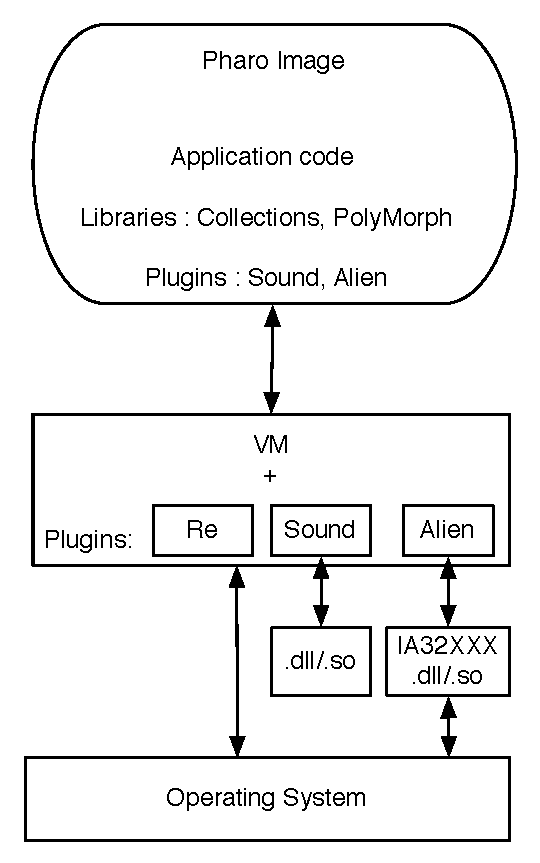
\includegraphics[width=0.4\linewidth]{figs/plugins.pdf}
	\caption{Pharo Architecture}
	\label{fig:plugins}
\end{figure}

The Alien library uses the \emph{IA32ABI} plugin which ....



\section{Using the Alien Library} \label{sec:the_alien_library} % (fold)

\subsection{Installation} \label{sec:installation} % (fold)

Alien is a Squeaksource project \url{http://www.squeaksource.com/Alien}. 
Use the following code to install Alien in a Pharo 1.1 image:

\begin{code}{}
Gofer new
	url: 'http://www.squeaksource.com/Alien' ;
	package: 'ConfigurationOfAlien';
	load.

(Smalltalk at: #ConfigurationOfAlien) loadCore ; 
	loadTests ; 
	loadLibC.
\end{code}

Run the tests to ensure that Alien is well installed and that the VM plugin is correctly working.

\subsection{First example} \label{subsec:first_example} % (fold)




\subsection{Core Classes} 

Figure~\ref{fig:alien_uml} shows an UML diagram of the Alien-Core package that contains the main classes of this library.

\begin{figure}[htbp]
	\centering
		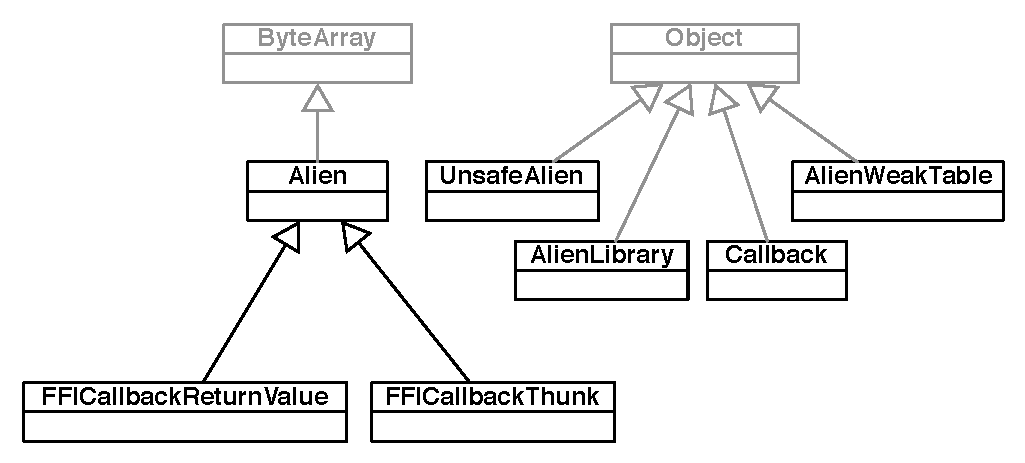
\includegraphics[width=0.9\linewidth]{figs/alien_uml}
	\caption{Core classes of the Alien library}
	\label{fig:alien_uml}
\end{figure}



\subsection{Memory management} \label{sec:memory_management} % (fold)


\subsection{Calling an external C library from Smalltalk} \label{sec:calling_an_external_c_library_from_smalltalk} % (fold)


\subsection{Callbacks from C to Smalltalk code} \label{sec:callbacks_from_c_to_smalltalk_code} % (fold)





\section{Dissection of Alien} \label{sec:dissection_of_alien} % (fold)


\paragraph{Alien}
% copy/past from class comment
% Instances of the Alien class represent actual parameters, return results and function pointers in FFI call-outs and call-backs and provide handles on external data.  See NewsqueakIA32ABIPlugin for the VM code that actually implements call-outs and call-backs.
% 
% 	See the class-side examples category for some simple example workspaces.
% 
% 	Aliens represent ABI (C language) data.  They can hold data directly in their bytes or indirectly by pointing to data on the C heap.  Alien instances are at least 5 bytes in length. The first 4 bytes of an Alien hold the size, as a signed integer, of the datum the instance is a proxy for.  If the size is positive then the Alien is "direct" and the actual datum resides in the object itself, starting at the 5th byte.  If the size is negative then the proxy is "indirect", is at least 8 bytes in length and the second 4 bytes hold the address of the datum, which is assumed to be on the C heap.  Any attempt to access data beyond the size will fail.  If the size is zero then the Alien is a pointer, the second 4 bytes hold a pointer, as for "indirect" Aliens, and accessing primitives indirect through the pointer to access data, but no bounds checking is performed.
% 
% 	When Aliens are used as parameters in FFI calls then all are "passed by value", so that e.g. a 4 byte direct alien will have its 4 bytes of data passed, and a 12-byte indirect alien will have the 12 bytes its address references passed.  Pointer aliens will have their 4 byte pointer passed.  So indirect and pointer aliens are equivalent for accessing data but different when passed as parameters, indirect Aliens passing the data and pointer Aliens passing the pointer.
% 
% 	Class Variables:
% 	GCMallocedAliens <AlienWeakTable of <Alien -> Integer>> - weak collection of malloced aliens, used to free malloced memory of Aliens allocated with newGC:
% 	LoadedLibraries <Dictionary of <String -> Alien>> - library name to library handle map
% 	

\paragraph{FFICallbackReturnValue} 
% copy/past from class comment
% An instance of FFICallbackReturnValue specifies a return value to be passed to a callback callee.  It is intended to have overlaid the following struct:
% 
% \begin{verbatim}
% /*
%  * Returning values from callbacks is done through a CallBackReturnSpec
%  * which contains a type tag and values.  It is designed to be overlaid upon
%  * an FFICallbackReturnProxy created at the Smalltalk level to return values.
%  */
% typedef struct {
%     long type;
% # define retint32  0 
% # define retint64  1
% # define retdouble 2
% # define retstruct 3
%     long _pad; /* so no doubt that valflt64 & valint32 et al are at byte 8 */
%     union {
%         long valint32;
%         struct { long low, high; } valint64;
%         double valflt64;
%         struct { void *addr; long size; } valstruct;
%     } rvs;
% } CallBackReturnSpec;
% \end{verbatim}


\paragraph{FFICallbackThunk} 
% copy/past from class comment

% An instance of FFICallbackThunk is a reference to a machine-code thunk/trampoline that calls-back into the VM.  The reference can be passed to C code which can use it as a function pointer through which to call-back into Smalltalk.  The machine-code thunk/trampoline is different for each instance, hence its address is a unique key that can be used to assocuate the Smalltalk side of the call-back (e.g. a block) with the thunk.  Since thunks must be executable and some OSs may not provide default execute permission on memory returned by malloc we may not be able to use malloc directly.  Instead we rely on a primitive to provide memory that is guaranteed to be executable.  The FFICallbackThunk class>>allocateExectablePage primitive answers an Alien that references an executable piece of memory that is some (possiby unitary) multiple of the pagesize.  Class-side code then parcels out pieces of a page to individual thunks.  These pieces are recycled when thunks are reclaimed.  Since the first byte of a thunk is non-zero we can use it as a flag indicating if the piece is in use or not.
% 
% See Callback for the higher-level construct that represents a Smalltalk block to be run in response to a callback.  Callbacks wrap instances of FFICallbackThunk and arbitrary Alien instances that describe the stack layout for receiving arguments.
% 
% Class Variables
% AccessProtect <Semaphore> critical section for ExecutablePages (de)allocation
% AllocatedThunks <AlienWeakTable of <FFICallbackThunk -> Integer>> - weak collection of thunks, used to return thunk storage to the executable page pool.
% ExecutablePages <Set of: Alien "executable page"> - collection of pages with execute permissions used to provide executable thunks


\paragraph{UnsafeAlien}
% copy/past from class comment

% Instances of UnsafeAlien represent the addresses of heap-resident non-pointer Smalltalk objects as actual parameters in FFI call-outs.  An UnsafeAlien on (e.g.) a ByteString used as a parameter in an FFI call causes the FFI machinery to pass the address of the first byte in the ByteString.  THIS IS UNSAFE!  It is unsafe because
% a) the garbage collector can potentially move the ByteString (or any other object) during the call, because the call may call-back, invoking the garbage collector,
% b) if external code retains the address for longer than the duration of the call and dereferences it in a subsequent call the object may have moved in the mean time,
% c) the address of the object is passed without any other potentially necessary conversions such as null-termination
% d) the hundred other problems this benighted author hasn't thought of.
% Hence UnsafeAlien is to be used carefully by clients that know that the usage is safe.
% You have been warned ;)
% 
% Create instances via
% 	UnsafeAlien forPointerTo: 'You are on your own!', (ByteString with: (Character value: 0))

\paragraph{AlienLibrary}
% copy/past from class comment

\paragraph{Callback}
% copy/past from class comment
% Callbacks encapsulate callbacks from the outside world.  They allow Smalltalk blocks to be evaluated and answer their results to external (e.g. C) callees.
% 
% Instance Variables:
% block <BlockContext> - The Smalltalk code to be run in response to external code invoking the callback.
% thunk <FFICallbackThunk> - the wrapper around the machine-code thunk that initiates the callback and whose address should be passed to C
% argsProxy <Alien> - the wrapper around the thunk's incomming stack pointer, used to extract arguments from the stack.
% resultProxy <FFICalbackReturnValue> - the specification of the block's return value and its C type so that the result can be passed back in the right low-level form.
% 
% Class Variables:
% ThunkToCallbackMap <Dictionary of: thunkAddress <Integer> -> callback <Callback>> - used to lookup the Callback associated with a specific thunk address on callback.  See FFICallbackThunk.

\paragraph{AlienWeakTable}
% copy/past from class comment

% This class supports simple post-mortem finalization of values associated with gc'ed objects.  An object to be finalized is registered in the table together with another object called 'the tag'. The finalizable object is held onto by the table weakly, the tag object--strongly. A table is initialized with the owner object, which is the object that performs the actual finalization. Some time after a finalizable object is garbage-collected, the owner is sent the \#finalize: message with the object's tag as the argument.
% 
% Instance Variables:
% 	accessProtect <Semaphore>  - A mutex protecting state
% 	firstUnusedIndex <Integer> - The lowest index in strongArray that is empty (an invariant)
% 	lastUsedIndex <Integer> - The highest index in strongArray that is not empty (an invariant)
% 	weakArray <WeakArray> - The array of objects whose death we're interested in.
% 	strongArray <Array> - The array of corresponding objects that wll be passed to the owner when their corresponding element in weakArray is garbage collected.
% 	owner <Object> - The object that is sent finalize: with the tag of an object that has been garbage-collected.
% 

\section{Study Case: the AlienOpenGL package} \label{sec:example_the_alienopengl_package} % (fold)


%=================================================================
\ifx\wholebook\relax\else\end{document}\fi
%=================================================================
